%                                     MMMMMMMMM                                         
%                                                                             
%  MMO    MM   MMMMMM  MMMMMMM   MM    MMMMMMMM   MMD   MM  MMMMMMM MMMMMMM   
%  MMM   MMM   MM        MM     ?MMM              MMM$  MM  MM         MM     
%  MMMM 7MMM   MM        MM     MM8M    MMMMMMM   MMMMD MM  MM         MM     
%  MM MMMMMM   MMMMMM    MM    MM  MM             MM MMDMM  MMMMMM     MM     
%  MM  MM MM   MM        MM    MMMMMM             MM  MMMM  MM         MM     
%  MM     MM   MMMMMM    MM   MM    MM            MM   MMM  MMMMMMM    MM
%
%
%            - META-NET Baltųjų knygų serija | Lietuvių kalba -

\documentclass[]{../metanetpaper}

\usepackage{booktabs}
\usepackage{longtable}
\usepackage{tabulary}
\usepackage{tabularx}
\usepackage{rotating}
\usepackage{makecell}
\usepackage{multirow}
\usepackage{colortbl}
\usepackage{polyglossia}
\usepackage{multicol,framed,lipsum}
\setotherlanguages{lithuanian,english}

%!TEX TS-program = xelatex
\RequireXeTeX %Force XeTeX check

\title{Lietuvių kalba skaitmeniniame amžiuje --- The Lithuanian Language in the Digital Age}

\subtitle{White Paper Series --- Baltųjų knygų serija}

\author{
  Aljoscha Burchardt \\
  Markus Egg \\
  Kathrin Eichler \\
  Brigitte Krenn \\
  Jörn Kreutel \\
  Annette Leßmöllmann \\
  Georg Rehm \\
  Manfred Stede \\
  Hans Uszkoreit \\
  Martin Volk \\
  Daiva Vaišnienė \\
  Jolanta Zabarskaitė
}
\authoraffiliation{
  Aljoscha Burchardt~ {\small DFKI}\\
  Markus Egg~ {\small Humboldt-Universität zu Berlin}\\
  Kathrin Eichler~ {\small DFKI} \\
  Brigitte Krenn~ {\small ÖFAI}\\
  Jörn Kreutel~ {\small FH Brandenburg}\\
  Annette Leßmöllmann~ {\small Hochschule Darmstadt}\\
  Georg Rehm~ {\small DFKI} \\
  Manfred Stede~ {\small Universität Potsdam}\\
  Hans Uszkoreit~ {\small Universität des Saarlandes, DFKI} \\
  Martin Volk~ {\small Universität Zürich} \\
  Daiva Vaišnienė ~ {\small Lietuvių kalbos institutas} \\
  Jolanta Zabarskaitė ~ {\small Lietuvių kalbos institutas}
}
\editors{
  Georg Rehm, Hans Uszkoreit\\(redaktoriai, \textcolor{grey1}{editors})
}

\begin{document}

\renewcommand*{\figureformat}{\sffamily\thefigure\autodot}

\maketitle

% ---------------- Mocktitle ------------------
\null
\pagestyle{empty} 

\centerline{META-NET -- office@meta-net.eu -- http://www.meta-net.eu}

\vfill

\begin{small}
  \selectlanguage{lithuanian}
  Šios Baltosios knygos sudarymas buvo finansuotas pagal Europos Komisijos septintąją bendrąją programą ir IKT politikos paramos programą: T4ME (subsidijų sutartis Nr. 249119), CESAR (subsidijų sutartis Nr. 271022), METANET4U (subsidijų sutartis Nr. 270893) ir META-NORD (subsidijų sutartis Nr. 270899).
\end{small}

\bigskip
\begin{small}
\selectlanguage{english}
  The development of this white paper has been funded by the Seventh
  Framework Programme and the ICT Policy Support Programme of the
  European Commission under the contracts T4ME (Grant Agreement 249119),
  CESAR (Grant Agreement 271022), METANET4U (Grant Agreement 270893)
  and META-NORD (Grant Agreement 270899).
\end{small}

\clearpage
% ------------- End of mocktitle ----------------

\pagenumbering{Roman} 
\setcounter{page}{5}
\pagestyle{scrheadings}

\cleardoublepage

% --------------------------------------------------------------------------

\bsection*{Įžanga --- Preface}

\begin{Parallel}[c]{78mm}{78mm}
\ParallelLText{\selectlanguage{lithuanin}
 Ši Baltoji knyga yra viena iš knygų serijos, skleidžiančios žinias apie kalbos technologijas (toliau – KT) ir jų galimybes. Ji skirta pedagogams, žurnalistams, politikams, kalbos vartotojų bendruomenėms ir pan.

Europos kalboms sukurtų bei pritaikytų technologijų skaičius ir jų pritaikymo lygmuo yra gana skirtingas. Žinoma, skiriasi ir veiksmai, kurių reikėtų imtis norint paskatinti konkrečios KT mokslinius tyrimus ir plėtrą. Šie veiksmai priklauso nuo daugelio veiksnių, tokių kaip kalbos sudėtingumas ir jos vartotojų skaičius.

META-NET, Europos Komisijos finansuojamas kompetencijos tinklas, šioje Baltųjų knygų serijoje atliko turimų kalbinių išteklių ir technologijų analizę, į kurią įtrauktos visos 23 oficialiosios bei kitos svarbios nacionalinės ir regioninės Europos kalbos (p.~\pageref{whitepaperseries}). Remiantis analizės rezultatais, konstatuotina, kad kiekvienos KT moksliniai tyrimai turi rimtų spragų. Ekspertų atlikta išsamesnė esamos padėties analizė ir įvertinimas galėtų padėti padidinti papildomų tyrimų poveikį ir sumažinti galimą riziką.

2011 metų lapričio mėnesio duomenimis, META-NET tinklą sudaro 33 šalyse veikiantys 54 mokslinių tyrimų centrai (p.~\pageref{metanetmembers}), bendradarbiaujantys su suinteresuotomis šalimis – verslo įmonių (programinės įrangos gamintojų, technologijų tiekėjų ir vartotojų), vyriausybės įstaigų, pramonės, tyrimų organizacijų, nevyriausybinių organizacijų, kalbos vartotojų bendruomenių ir Europos universitetų atstovais. Dirbdamas kartu su šiomis bendruomenėmis META-NET kuria bendrą technologijų viziją ir rengia strateginę mokslinių tyrimų darbotvarkę 2020 metų daugiakalbei Europai.}

\ParallelRText{\selectlanguage{english}
This white paper is part of a series that promotes knowledge about language technology and its potential. It addresses journalists, politicians, language communities, educators and others. 

The availability and use of language technology in Europe varies between languages. Consequently, the actions that are required to further support research and development of language technologies also differ. The required actions depend on many factors, such as the complexity of a given language and the size of its community.

META-NET, a Network of Excellence funded by the European Commission, has conducted an  analysis of current language resources and technologies in this white paper series (p.~\pageref{whitepaperseries}). The analysis focused on the 23 official European languages as well as other important national and regional languages in Europe. The results of this analysis suggest that there are tremendous deficits in technology support and significant research gaps for each language. The given detailed expert analysis and assessment of the current situation will help maximise the impact of additional research.

As of November 2011, META-NET consists of 54 research centres from 33 European countries (p.~\pageref{metanetmembers}). META-NET is working with stakeholders from economy (software companies, technology providers, users), government agencies, research organisations, non-governmental organisations, language communities and European universities. Together with these communities, META-NET is creating a common technology vision and strategic research agenda for multilingual Europe 2020.} 
\ParallelPar
\end{Parallel}

% --------------------------------------------------------------------------

\cleardoublepage

\bsection*{Turinys --- Table of Contents}

\tableofcontents

\addtocontents{toc}{\protect\thispagestyle{empty}\protect}
\addtocontents{toc}{{\Large\textsf{\centerline{LIETUVIŲ KALBA SKAITMENINIAME AMŽIUJE}}\par}}

% --------------------------------------------------------------------------

\cleardoublepage

\setcounter{page}{1}
\pagenumbering{arabic} 
\pagestyle{scrheadings}

\ssection[Santrauka]{Santrauka}

\selectlanguage{lithuanian}

\begin{multicols}{2}
 Per pastaruosius 60 metų Europa įgijo aiškią politinę ir ekonominę struktūrą, tačiau kultūros ir kalbų požiūriu ji vis dar labai skirtinga. Taigi nuo portugalų iki lenkų, nuo italų iki islandų – kiekvieną dieną bendraudami visuomenės, verslo ir politikos srityse Europos piliečiai neišvengiamai susiduria su kalbų barjerais. Europos Sąjungos institucijos per metus išleidžia apie milijardą eurų daugiakalbystės politikai įgyvendinti, verčiant tekstus raštu ir žodžiu. Tačiau ar ši našta turėtų būti tokia milžiniška? Šiuolaikinės  ir moksliniai kalbų tyrimai gali labai padėti griaunant tokius kalbų barjerus. KT, įdiegtos išmaniuosiuose prietaisuose ir programose, ateityje galės padėti europiečiams lengvai susikalbėti ir bendradarbiauti, net jei jie kalba skirtingomis kalbomis. 

\boxtext{Kalbos technologijos tiesia tiltus}

 Lietuvos ūkis turi didžiulės naudos iš Europos bendrosios rinkos: 2010 metais prekyba su Europos Sąjunga sudarė 61 proc., o su kitomis Europos šalimis – dar 3 proc. viso Lietuvos eksporto. Tačiau kalbų barjerai gali stabdyti verslą, ypač jei kalbame apie mažas ir vidutinio dydžio įmones, neturinčias lėšų pakeisti situaciją. Vienintelė (neįsivaizduojama) alternatyva tokiai daugiakalbei Europai būtų leisti įsigalėti vienai kalbai, kuri ilgainiui pakeistų visas kitas kalbas.

Klasikinis būdas įveikti kalbų barjerus – mokytis užsienio kalbų. Tačiau išmokti 23 oficialiąsias ir dar beveik 60 kitų Europos kalbų nesinaudojant technologijomis europiečiams būtų neįveikiama užduotis bei kliūtis siekiant Europos ekonominės, politinės ir mokslinės pažangos. 

Geriausia išeitis – kurti plačių galimybių technologijas (angl. \textit{key enabling technology}). Jos suteikia rinkos dalyviams didžiulio pranašumo ne tik Europos bendrojoje rinkoje, bet ir palaikant prekybinius ryšius su trečiųjų šalių besivystančiomis rinkomis. Norint pasiekti šį tikslą, išsaugoti Europos kultūrinę ir kalbinę įvairovę, būtina pirmiausia sistemiškai išanalizuoti visų Europos kalbų ypatybes ir nustatyti joms pritaikytų KT būklę.  

Šiuo metu rinkoje turimi automatinio vertimo ir šnekamosios kalbos apdorojimo įrankiai – tai tik šio ambicingo tikslo siekimo pradžia. Pagrindinės šios srities lyderės – Šiaurės Amerikoje įsikūrusios privačios pelno siekiančios įmonės. Europos Sąjunga jau aštuntojo dešimtmečio pabaigoje suprato KT svarbą kuriant vieningą Europą ir ėmė finansuoti pirmuosius mokslinių tyrimų projektus, tokius kaip EUROTRA. Tuo metu buvo parengta nacionalinių projektų, kuriuos įgyvendinus buvo pasiekta vertingų rezultatų, tačiau visos Europos mastu veiksmai taip ir nebuvo koordinuojami. O tuo tarpu kitose daugiakalbėse bendruomenėse, tokiose kaip Indijos (22 oficialiosios kalbos) ir Pietų Afrikos (11 oficialiųjų kalbų), pastaruoju metu pradėtos įgyvendinti kalbos mokslinių tyrimų ir technologijų plėtros nacionalinės programos.

Šiandien pagrindiniai kalbų technologijų rinkos dalyviai remiasi ne itin tobulais statistiniais metodais, kurie nėra pagrįsti nuodugnesniais lingvistiniais metodais ir išsamesnėmis žiniomis. Pavyzdžiui, sakiniai automatiškai verčiami lyginant naują sakinį su tūkstančiais kitų sakinių, kuriuos jau yra išvertę vertėjai. Rezultato kokybė labai priklauso nuo turimo pavyzdžių tekstyno dydžio ir kokybės. Nors paprastų sakinių automatinis vertimas tomis kalbomis, kuriomis sukaupta pakankamas kiekis tekstų, gali būti vertingas, susidūrus su kalbomis, kurių teksto pavyzdžių sukaupta gerokai mažiau, arba verčiant sudėtingos struktūros sakinius, paviršutiniški statistiniai metodai pasirodys netinkami. Gilesnių struktūrinių kalbos savybių analizė yra vienintelis būdas judėti į priekį, jei norime kurti programas, pritaikytinas visoms Europos kalboms.

\boxtext{Kalbos technologijos – ateities raktas}

Europos Sąjunga yra nusprendusi finansuoti tokius projektus kaip \textit{EuroMatrix }  ir \textit{EuroMatrixPlus} (projektai pradėti įgyvendinti 2006 metais) bei \textit{ iTranslate4} (2010 metais), kurių metu atliekami fundamentalieji ir taikomieji moksliniai tyrimai, kuriami ištekliai, skirti visų Europos kalbų kokybiškiems KT sprendiniams.

 Šios srities tyrimai Europoje yra gana sėkmingi. Pavyzdžiui, Europos Sąjungos vertimų tarnybos šiuo metu naudojasi atvirąja automatinio vertimo programine įranga MOSES, sukurtą įgyvendinant europinius mokslinių tyrimų projektus. VERBMOBIL projektas, Vokietijos švietimo ir mokslo ministerijos finansuotas 1993–2000 m.,  padarė Vokietiją šnekamosios kalbos vertimo lydere pasaulyje. Daug tyrimų ir plėtros laboratorijų, tuo metu įsikūrusių Vokietijoje (pvz., IBM ir „Philips“), vėliau buvo uždarytos ar perkeltos kitur. Deja, Europa nepasinaudojo šių projektų rezultatais tolesniems darbams, bet pasirinko pavienius mokslinius tyrimus, kurių įtaka rinkai nėra tokia reikšminga. Vis dėlto net pačių pirminių pastangų ekonominę naudą atspindi gausybė sukurtų papildomų produktų. 1984 m. įsteigta bendrovė „Trados“ 2005 m. buvo parduota Jungtinėje Karalystėje įsikūrusiai bendrovei SDL.

\boxtext{Kalbos technologijos padeda Europai vienytis}

Remiantis ligšiolinėmis įžvalgomis galima daryti išvadą, kad dabartinės „hibridinės“ KT, jungiančios giluminį duomenų apdorojimą ir statistinius metodus, sugebės nutiesti tiltus tarp visų Europos kalbų ir pasiekti dar geresnių rezultatų. Kaip galima suprasti perskaičius šią Baltųjų knygų seriją,  Europos šalių pasirengimas taikyti kalbinius sprendinius ir jų vykdomų mokslinių tyrimų lygis smarkiai skiriasi. Norint sukurti tikrai veiksmingų, kasdieniam vartojimui skirtų KT, Lietuvai reikės atlikti dar nemažai mokslinių tyrimų. Proveržiai KT srityje skatintų jų diegimą versle, padėtų plėsti ir gerinti viešąsias paslaugas ir pan., taip pat suteiktų galimybę lietuvių kalbą vartoti visose gyvenimo srityse  komunikacijos terpėse. 

Tinklo META-NET ilgalaikis uždavinys – pristatyti kokybiškas KT, taikomas visoms Europos kalboms, siekiant kultūrine įvairove pagrįstos politinės ir ekonominės vienybės. Šios technologijos padės sugriauti dabartinius barjerus ir nutiesti tiltus tarp Europos kalbų. Visos suinteresuotosios šalys – politikai, tyrėjai, verslo ir visuomenės atstovai – turi suvienyti savo pastangas, kurdami bendrą ateitį.

Ši Baltųjų knygų serija papildo kitus tinklo META-NET strateginius veiksmus, apžvelgiamus šio dokumento priede. Aktualios informacijos, pavyzdžiui, tinklo META-NET vizijos dokumento naujausią versiją \cite{Meta1} arba strateginių mokslinių tyrimų darbotvarkę galima rasti tinklo META-NET tinklalapyje: http://www.meta-net.eu.
\end{multicols}

\clearpage

% --------------------------------------------------------------------------

\ssection[Grėsmės kalbai: iššūkis kalbos technologijoms]{Grėsmės kalbai:\newline  iššūkis kalbos technologijoms}

\begin{multicols}{2}

Gyvename skaitmeninės revoliucijos, turinčios didžiulį poveikį bendravimui ir visuomenės raidai, metu. Naujausi skaitmeninės informacijos pateikimo ir bendravimo technologijų išradimai kartais prilyginami Johanneso Gutenbergo spausdinimo mašinos išradimui. Ką ši analogija gali byloti apie Europos informacinės visuomenės ir ypač apie mūsų kalbų ateitį?

\boxtext{Esame skaitmeninės revoliucijos liudininkai. Ši revoliucija prilygsta Gutenbergo spausdinimo mašinos išradimui.}

Gutenbergo išradimas lėmė svarbius proveržius komunikacijos ir žinių mainų srityje, tokius kaip Martino Lutherio atliktą Biblijos vertimą į gimtąją kalbą ir kt. Vėlesniais amžiais buvo sukurta kultūrinių metodologijų, lengvinančių kalbos apdorojimą ir žinių mainus:

\medskip
\begin{itemize}
\item Ortografinis ir gramatinis labiausiai paplitusių kalbų standartizavimas suteikė galimybių sparčiau plisti naujoms mokslinėms ir intelektinėms idėjoms.
\item Bendrinių kalbų susiformavimas suteikė piliečiams galimybių bendrauti tam tikruose (dažniausiai politinių valstybių sienų apibrėžtuose) plotuose.
\item Kalbų mokymas ir vertimai iš vienos kalbos į kitą suteikė galimybių keistis informacija skirtingomis kalbomis.
\item Redagavimo ir bibliografinės gairės užtikrino spausdintos informacijos kokybę bei prieinamumą.
\medskip
\item Skirtingų žiniasklaidos priemonių – laikraščių, radijo, televizijos, knygų ir kitokių – atsiradimas tenkino skirtingus komunikavimo poreikius.
\end{itemize}

Per pastarąjį dvidešimtmetį informacinės technologijos padėjo automatizuoti ir palengvinti daugybę procesų:

\begin{itemize}
\item Kompiuterinė programinė įranga pakeitė spausdinimą mašinėle ir rankinį tekstų rinkimą.
\item Programa \textit{ Microsoft PowerPoint} pakeitė projektoriumi rodomas skaidres.
\item Elektroniniu paštu siųsti ir gauti dokumentus galime sparčiau nei faksu.
\item Programa \textit{Skype} teikia galimybę pigiai skambinti internetu ir rengti virtualius susitikimus.
\item Garso ir vaizdo kodavimo formatai palengvina daugialypės terpės turinio keitimą.
\item Paieškos sistemos teikia galimybių naudojant esminius žodžius pasiekti reikiamus tinklalapius.
\item Internetinės paslaugos, tokios kaip \textit{Google Translate}, teikia galimybių sparčiai, nors ir ne visada tiksliai, versti tekstus.
\item Socialinės terpės, tokios kaip \textit{Facebook}, \textit{Twitter} ir \textit{Google+}, lengvina bendravimą, bendradarbiavimą ir keitimąsi informacija.
\end{itemize}

Nors tokios priemonės ir programos yra naudingos, kol kas jos nepajėgia išlaikyti visapusiškai tvarios daugiakalbės Europos visuomenės, kurioje galėtų vykti netrikdoma informacijos ir prekių sklaida.

\subsection{Kalbų barjerai - kliuvinys Europos informacinei visuomenei}
  
 Negalime tiksliai numatyti, kokia bus ateities informacinė visuomenė. Tačiau tikėtina, kad komunikacinių technologijų revoliucija skirtingomis kalbomis kalbantiems žmonėms teikia naujų būdų suartėti. Dėl to žmonės patiria spaudimą mokytis naujų kalbų, o programinės įrangos kūrėjai – kurti naujus technologinius sprendinius, kurie užtikrintų susikalbėjimą ir prieigą prie bendrų žinių. Dėl naujų medijų rūšių pasaulinėje ekonominėje ir informacinėje erdvėje sąveikauja vis daugiau kalbų ir jomis kalbančių žmonių informacijos. 

\boxtext{Pasaulinėje ekonominėje ir informacinėje erdvėje sąveikauja vis daugiau kalbų ir jomis kalbančių žmonių informacijos.}

Šiuo metu išpopuliarėjusios bendrauti skirtos priemonės (\textit{Wikipedia}, \textit{Facebook}, \textit{Twitter}, \textit{YouTube} ir visai neseniai – \textit{Google+}) yra vos ledkalnio viršūnė.

Šiandien galime akimirksniu iš kito pasaulio krašto parsisiųsti keletą gigabaitų teksto ir tik po to pamatyti, kad jis parašytas kalba, kurios nesuprantame. Anot vienos iš Europos Komisijos pastarojo laikotarpio ataskaitų, 57 proc. interneto naudotojų Europoje perka prekes ir paslaugas ne savo gimtąja kalba (anglų kalba yra labiausiai paplitusi užsienio kalba, po jos – prancūzų, vokiečių ir ispanų kalbos). 55 proc. naudotojų skaito internete pateikiamą informaciją užsienio kalbomis ir vos 35 proc. užsienio kalbomis rašo elektroninius laiškus arba komentarus interneto tinklalapiuose \cite{EC1}.  Prieš kelerius metus anglų kalba gal ir buvo interneto \textit{lingua franca}  – didžioji dalis internete pateikiamos informacijos buvo ja parašyta – tačiau dabar padėtis radikaliai pasikeitė. Internetą užplūdo informacija kitomis Europos, taip pat Azijos ir Vidurio Rytų kalbomis. 

Neįtikėtina, bet atrodo, kad ši skaitmeninė takoskyra dėl kalbų barjerų nesulaukė labai daug visuomenės dėmesio. Tačiau ji kelia itin aktualų klausimą: kurios Europos kalbos klestės į tinklą sujungtoje informacinėje ir žinių visuomenėje, o kurioms lemta išnykti?

\subsection{Grėsmė kalboms }

Nors spausdinimo mašina ir palengvino keitimąsi informacija, tai lėmė kai kurių Europos kalbų išnykimą. Spaudinių regioninėmis ir mažumos kalbomis buvo mažai, o tokios kalbos kaip kornų ir dalmatų išvis neturėjo raštijos ir tai labai apribojo  jų vartojimo sritis. Ar ir interneto poveikis mūsų kalboms bus toks pats?

Europoje kalbama apie 80 kalbų. Jos yra vienas iš gausiausių ir svarbiausių  regiono kultūros turtų bei esminė Europos unikalaus socialinio modelio dalis \cite{EC2}.  Nors tokios kalbos kaip anglų ir ispanų greičiausiai išliks besivystančioje skaitmeninėje rinkoje, daugelis Europos kalbų gali tapti nereikalingos į tinklą susietoje visuomenėje. Tai susilpnintų Europos padėtį pasaulyje ir pakenktų strateginiam tikslui užtikrinti kiekvieno Europos piliečio neatsižvelgiant į vartojamą kalbą galimybes būti visateisiu Sąjungos nariu.  

\boxtext{Europos kalbų įvairovė – svarbi jos kultūros turto dalis.}

Anot UNESCO ataskaitos apie daugiakalbystę, kalbos sudaro esminę terpę džiaugtis pamatinėmis teisėmis, tokiomis kaip teisė į politinę raišką, švietimą ir dalyvavimą visuomenės gyvenime \cite{Unesco1}.

\subsection{Kalbos technologijos – naujų galimybių kūrėjos}

Anksčiau investicijos ir pastangos išsaugoti kalbų įvairovę buvo skiriamos kalbų mokymui ir vertimams. Apytikriais skaičiavimais, 2008 m. Europos vertimų raštu ir žodžiu, programinės įrangos lokalizavimo ir internetinių tinklalapių vertimo rinkos vertė sudarė 8,4 mlrd. eurų, tikėtinas jos metinis augimas yra 10 proc.\cite{EC3}.  Deja, šie skaičiai atspindi tik nedidelę dalį dabartinio ir būsimo poreikio bendrauti skirtingomis kalbomis. Pagrindinis būdas užtikrinti kalbų vartojimo plėtrą ir sklaidą rytdienos Europoje – pasitelkti tinkamas technologijas. Juk būtent technologijos padeda mums tenkinti transporto, energetinius ir kitokius poreikius.

Skaitmeninės KT (skirtos visoms rašomosios ir šnekamosios kalbos formoms) padeda žmonėms bendradarbiauti, dirbti, dalytis žiniomis ir dalyvauti socialinėse bei politinėse diskusijose, nepaisant kalbų barjerų ar darbo kompiuteriu įgūdžių. Šios technologijos neretai būna nepastebimos sudėtingų programinės įrangos sistemų dalys, padedančios:

\begin{itemize}
\item rasti informacijos naudojantis internetinės paieškos sistema;
\item patikrinti, ar tekste nėra rašybos, skyrybos ir gramatinių klaidų;
\item peržiūrėti produktų rekomendacijas internetinėje parduotuvėje;
\item suprasti automobilio navigacinės sistemos žodines instrukcijas;
\item versti tinklalapius naudojant internetines programas.
\end{itemize}

KT sudaro aibė pagrindinių programų, veikiančių didesnėse programinės įrangos sistemose. META-NET Baltųjų knygų tikslas – apžvelgti, kaip šios pagrindinės programos yra išplėtotos ir pritaikytos kiekvienai iš Europos kalbų. 

\boxtext{Europai reikia stabilių, lengvai prieinamų kalbos technologijų, pritaikytų visoms Europos kalboms.}

Jei norės neprarasti pozicijos tarp pasaulio inovacijų lyderių, Europai reikės stabilių, lengvai prieinamų ir į svarbiausias programinės įrangos terpes integruotų KT, pritaikytų visoms Europos kalboms. Neturėdami reikiamo lygio KT, artimiausioje ateityje nesugebėsime užtikrinti kalbos vartotojams interaktyvaus daugiakalbio bendravimo daugialypėje terpėje.

\subsection{Kalbos technologijų galimybės}

Spausdinto žodžio pasaulyje didysis technologinis proveržis buvo galimybė greitai kopijuoti vaizdą ar tekstą  tinkamo galingumo spausdinimo mašina. Žmonėms teko sunkus darbas – ieškoti žinių, jas skaityti, versti ir apibendrinti. Mes norėjome laukti Thomo Edisono išradimų, padėjusių įrašyti šnekamąją kalbą. Ši technologija suteikė galimybių gaminti analogines kopijas.

Dabar turint skaitmeninių technologijų galima automatizuoti vertimą, informacijos kūrimą ir žinių tvarkymą visomis Europos kalbomis. Be to, jos gali būti pritaikytos kuriant intuityvias kalbos / šnekos pagrindu veikiančias buities elektronikos, mechanizmų, transporto priemonių, kompiuterių ir robotų sąsajas. Verslo ir pramonės programos vis dar yra ankstyvosios plėtros lygmens, tačiau mokslinių tyrimų ir taikomosios veiklos pažanga atveria naujų galimybių. Pavyzdžiui, konkrečių sričių tekstų automatinis vertimas jau dabar yra gana tikslus, o eksperimentinės programos teikia galimybių tvarkyti informaciją ir žinias bei kurti naują turinį daugeliu Europos kalbų. 

 Kaip ir daugumos technologijų atveju, pirmosios kalbinės programos, pavyzdžiui, balsu valdomos naudotojų sąsajos ir dialogų sistemos, buvo skirtos itin specializuotoms sritims, jų veikimas gana ribotas. Tačiau švietimo ir pramogų rinkoje esama didžiulių galimybių diegti KT žaidimams, kultūrinio paveldo sąvokoms, mokomosioms ir pramoginėms priemonėms, bibliotekoms, imitacinėms aplinkoms ir mokomosioms programoms. Mobiliosios informavimo paslaugos, kompiuterinė programinė kalbų mokymo įranga, e.mokymo aplinka, vertinimo priemonės ir programos plagiatui aptikti, tai vos kelios sritys, kuriose KT gali būti ypač vertingos. Tokių daugialypės terpės bendravimo platformų kaip \textit{Twitter} ir \textit{Facebook} populiarumas leidžia manyti, kad ateityje prireiks ir pažangių KT, skirtų stebėti dalyvių žinutes, apibendrinti diskusijas, rodyti nuomonių tendencijas, aptikti emocingus atsakymus, nustatyti autorių teisių pažeidimus arba susekti netinkamo naudojimo atvejus.

\boxtext{Kalbos technologijos padeda įveikti kalbų įvairovės „negalią“.} 

KT teikia daug galimybių Europos Sąjungai. Jos gali padėti išspręsti sudėtingą Europos daugiakalbystės problemą – skirtingos kalbos gali kartu gyvuoti Europos įmonėse, organizacijose ir mokyklose. Gyventojai turi bendrauti be Europos bendrąją rinką skaidančių kalbų barjerų, o KT gali padėti jiems įveikti šią  kliūtį bei teikti daugiau galimybių laisvai ir viešai kalbėti savomis kalbomis. Žvelgiant dar toliau į priekį, Europos novatoriškos daugiakalbės technologijos pažymės gaires mūsų tarptautiniams partneriams, pradėsiantiems kurti technologijas savoms daugiakalbėms bendruomenėms. KT gali būti vertinamos kaip „pagalbinės“, padedančios visiems įveikti kalbų įvairovės „negalią“ ir suteikiančios skirtingoms kalbos vartotojų bendruomenėms daugiau galimybių bendrauti. Galiausiai viena iš aktualių mokslinių tyrimų sričių yra KT pritaikymas vykdant gelbėjimo operacijas nelaimių zonose, kur kiekvienas veiksmas gali lemti gyvybę ir mirtį: ateityje sumanieji robotai, galintys bendrauti įvairiomis kalbomis, turės daug daugiau galimybių gelbėti gyvybes. 

\subsection{Iššūkiai, kuriuos turi įveikti kalbos technologijos}

Nors KT pastaraisiais metais padarė nemažą pažangą, dabartiniai technologinės pažangos ir produkcijos naujovių taikymo tempai yra pernelyg lėti. Plačiau taikomos tekstų rašymo sistemų rašybos ir gramatikos tikrintuvės paprastai yra vienakalbės, o ir įdiegtos toli gražu ne visoms kalboms.

\boxtext{Šiuo metu technologinė pažanga yra pernelyg lėta.}

Internetinės automatinio vertimo paslaugos yra naudingos, kai norima greitai gauti apytikslį dokumento turinio vertimą, tačiau susiduriama su sunkumais, kai reikia itin tikslaus ir išsamaus vertimo. Dėl natūraliosios kalbos sudėtingumo kalbų modeliavimas programinėje įrangoje ir jų testavimas realioje aplinkoje yra ilgas, brangus procesas, kurį reikia nuolat finansuoti. Vis dėlto Europa privalo išsaugoti lyderės pozicijas spręsdama daugiakalbės bendruomenės technologines problemas ir rasti naujų būdų spartinti plėtrą visose srityse. Metodai galėtų būti susiję tiek su pažanga skaitmeninėje (kompiuterių) srityje, tiek su tokiomis metodikomis kaip individualių užduočių perdavimas žmonių grupėms ar bendruomenei (angl. \textit{crowdsourcing}).

\subsection{Kalbos įvaldymas: žmonės ir mašinos}

Norėdami suprasti, kaip kompiuteriai „išmoksta“ kalbą ir kodėl juos taip sunku užprogramuoti ją vartoti, trumpai pažvelkime į tai, kaip pirmąją ir antrąją kalbą išmoksta žmonės, o po to – kaip veikia KT sistemos.

\boxtext{Žmonės įgyja kalbos įgūdžių dvejopai: mokydamiesi iš pavyzdžių ir mokydamiesi pagrindinių kalbos taisyklių.}

Žmonės įgyja kalbos įgūdžių dviem skirtingais būdais. Kūdikiai išmoksta kalbą girdėdami, kaip bendrauja jų tėvai, broliai, seserys ir kiti šeimos nariai. Dvejų metų amžiaus vaikai pradeda patys kalbėti – iš pradžių tai būna atskiri žodžiai ir trumpos frazės. Tai įmanoma  todėl, kad žmonės  genetiškai gali mėgdžioti ir praktiškai taikyti, ką išgirdo.

Vyresnio amžiaus vaikams išmokti antrąją kalbą yra kiek sunkiau, ypač jeigu vaikas auga bendruomenėje, kuriai ta antroji kalba nėra gimtoji. Mokyklose paprastai mokoma užsienio kalbos gramatinės struktūros, žodyno ir rašybos taisyklių, t.~y.~atliekami pratimai, kuriais kalbos žinios įtvirtinamos pagal abstrakčias taisykles, lenteles ir pavyzdžius. 

Dviejų pagrindinių tipų KT sistemos kalbos išmoksta panašiais būdais. Statistiniais (arba pagrįstais duomenimis) metodais duomenys surenkami iš gausybės konkrečių tekstų pavyzdžių. Vienakalbiai tekstai gali būti naudojami tos pačios kalbos mokymo tikslais, pavyzdžiui, tikrinti, ar nėra rašybos klaidų, tačiau automatinio vertimo sistemai „išmokyti“ būtini lygiagretūs tekstai dviem ar daugiau kalbų. Iš tokių tekstų automatinio vertimo algoritmas „išmoksta“ žodžių, trumpų frazių ir visų sakinių vertimo modelius. 

Tokiam statistiniais metodais pagrįstam vertimui gali prireikti milijonų sakinių, o vertimo kokybė gerėja didėjant išanalizuotų tekstų kiekiui. Tai viena iš priežasčių, kodėl paieškos sistemų teikėjai pageidauja sukaupti kaip galima daugiau rašytinės informacijos. Tekstų rašymo ir tokių paslaugų kaip \textit{Google Search} ir \textit{Google Translate} rašybos klaidų taisymo funkcijos pagrįstos statistiniais metodais. Didžiausias statistikos pranašumas yra tas, kad mašina „mokosi“ greitai, įveikdama nesibaigiančius mokomuosius ciklus, nors kartais kokybė gali būti labai įvairi.

Antrasis KT ir ypač automatinio vertimo metodas yra kurti taisyklėmis pagrįstas sistemas. Lingvistikos, kompiuterinės lingvistikos ir kompiuterių mokslo ekspertai visų pirma turi užkoduoti gramatinę analizę (vertimo taisykles) ir sudaryti žodyno sąrašus (leksikonus). Tam reikia daug pastangų, intensyvaus darbo ir laiko. Kai kurios pagrindinės taisyklėmis pagrįstos automatinio vertimo sistemos buvo tobulinamos daugiau nei du dešimtmečius. Pagrindinis taisyklėmis pagrįstų sistemų pranašumas yra tas, kad ekspertai gali geriau kontroliuoti kalbos apdorojimą. Tai leidžia nuosekliai taisyti programinės įrangos klaidas ir palaikyti grįžtamąjį ryšį su naudotoju, ypač tuo atveju, kai taisyklėmis pagrįstos sistemos taikomos kalbų mokymui. Tačiau dėl didelių finansinių sąnaudų taisyklėmis pagrįstų KT turi susikūrusios tik didžiosios kalbos. 

Kadangi paprastai statistinių ir taisyklėmis pagrįstų sistemų pranašumai ir trūkumai kompensuoja vieni kitus, šiuo metu atliekami tyrimai siekiant sukurti hibridinius būdus, sujungsiančius šias dvi metodologijas. Tačiau kol kas didesnės sėkmės pasiekta ne taikant šiuos metodus verslo poreikiams, bet tyrimų laboratorijose. 

Taigi galima konstatuoti, kad didžioji dalis programų, kurias šiuo metu naudoja informacinė visuomenė, labai priklauso nuo KT. Tai ypač pasakytina apie Europos ekonominę ir informacinę erdvę su jos daugiakalbe bendruomene. Nors pastaraisiais metais KT srityje padaryta reikšminga pažanga, vis dar egzistuoja daugybė galimybių gerinti KT sistemų kokybę. Kituose skyriuose aptarsime lietuvių kalbos vietą Europos informacinėje visuomenėje ir įvertinsime dabartinę lietuvių KT būklę.
\end{multicols}

\clearpage

% --------------------------------------------------------------------------

\ssection[Lietuvių kalba Europos  informacinėje visuomenėje]{Lietuvių kalba \newline Europos  informacinėje  \newline visuomenėje}

\begin{multicols}{2}

\subsection{Bendrieji duomenys }

 Lietuvių kalba yra viena iš mažiau vartojamų Europos kalbų – ja kalba apie 4 mln. žmonių, dauguma jų gyvena Lietuvos Respublikoje. Valstybinė lietuvių kalba yra bendra rašomoji ir šnekamoji visiems Lietuvos Respublikos piliečiams, kurių, 2011 m. duomenimis, yra apie 3,2 mln., iš jų lietuvių tautybės – apie 2,7 mln.  

84 proc. Lietuvos gyventojų yra lietuviai, 6,1 proc. – lenkai, 4,9 proc. – rusai, 1,1 proc. – baltarusiai, 0,6 proc. – ukrainiečiai, dar po 0,1 proc. sudaro žydų, vokiečių, latvių, totorių, karaimų kilmės piliečiai. Be to, Lietuvoje gyvena apie 3 tūkst. romų bendruomenė, kurios didžiausia koncentracija yra Vilniaus regione (2001 m. surašymo duomenimis). Deja, nuo 2007 m. Lietuvos gyventojų skaičius kasmet mažėja. Šiuos pokyčius lemia mažėjantis gimstamumas bei emigracija, mažinanti Lietuvoje gyvenančių kalbos vartotojų skaičių.

Kiek lietuviškai kalbančiųjų yra pasaulyje, gana sudėtinga nustatyti. Spėjama, kad užsienyje gali gyventi per 500 tūkst. lietuviškai kalbančiųjų, kituose šaltiniuose nurodoma, kad ne mažiau nei 15 proc. kalbėtojų. Lietuvių kalba šneka lietuvių tautinės mažumos, gyvenančios Baltarusijoje, Lenkijoje, Latvijoje, bei didelės emigrantų bendruomenės JAV, Kanadoje, Jungtinėje Karalystėje, Airijoje, Ispanijoje, Pietų Amerikoje ir kitur. Pagal kalbančiųjų skaičių lietuvių kalba užima 144 vietą pasaulyje.  

\boxtext{Lietuvių kalba yra viena iš mažiau vartojamų Europos kalbų. Ja kalba vos apie 4 mln. žmonių, dauguma jų gyvena Lietuvos Respublikoje.} 

 Lietuvių kalba priklauso indoeuropiečių kalbų šeimos baltų šakai. Jos artimiausia giminaitė yra latvių kalba, kuria kalbama kaimyninėje Latvijoje.   

Pagal socialinės Europos kalbų raidos istoriją, kalbas skirstant į dominuojančiąsias ir dominuojamąsias, lietuvių kalba priskirtina prie antrųjų. Dominuojančiosios kalbos vieną tarmę bendrinėms kalboms formuoti paprastai buvo pasirinkusios ne vėliau kaip Renesanso laikotarpiu (anglų, prancūzų, italų, portugalų), o dominuojamosios susiformavo XIX amžiuje, Tautų pavasario metu (bulgarų, kroatų, lietuvių, slovakų). Bendrinė lietuvių kalba susiformavo XIX amžiaus pabaigoje – XX amžiaus pradžioje.   

Lietuvių kalbai būdinga didelė regioninių kalbos atmainų įvairovė. Dvi pagrindinės tarmės – aukštaičių ir žemaičių – skiriasi ne tik fonetinėmis ypatybėmis, bet ir gramatika bei leksika. Šios tarmės skirstomos į keturiolika stambesnių regioninių patarmių, o šios – į smulkesnių teritorinių vienetų šnektas. Patarmės viena nuo kitos skiriasi garsais, žodžių formomis ir kitokiomis savybėmis.

Bendrinė lietuvių kalba susiformavo XX amžiaus pradžioje vienos iš aukštaičių patarmių pagrindu, tačiau regioninis tapatumas ir tarminiai skirtumai vis dar labai ryškūs.

Nuo 1995 metų gestų kalba oficialiai pripažinta Lietuvos Respublikos kurčiųjų gimtąja kalba. Nuo to laiko lietuvių gestų kalba vystosi kaip nepriklausoma kalba.

\subsection{Lietuvių kalbos ypatybės}

 XIX amžiuje indoeuropeistai išgarsino stebėtiną lietuvių kalbos panašumą į sanskritą, ja imta didžiuotis kaip mažiausiai pakitusios struktūros gyvąja indoeuropiečių kalba. Dėl tos priežasties besimokantys klasikines Europos kalbas (lotynų, senąją graikų) lengviau supranta lietuvių kalbos gramatiką. Lietuvoje didžiuojamasi prancūzų lingvisto Antoine’o Meillet posakiu, jog kiekvienas, norintis išgirsti, kaip kalbėjo indoeuropiečių protėviai, turi važiuoti pasiklausyti lietuvio valstiečio.

Lietuvių kalba – pati konservatyviausia iš indoeuropiečių gyvųjų kalbų, jai pavyko geriausiai išsaugoti daugelį savo archajiškų savybių. Tipologijos požiūriu, lietuvių kalba yra svarbi dėl daugybės unikalių savybių, įskaitant gausias kaitybos formas, charakteringą toninio ir dinaminio kirčio sintezę bei itin įvairialypę žodžių tvarką, atspindinčią sudėtingus diskurso bendravimo ir sintaksinio lygmens santykius.

Rašomojoje lietuvių kalboje milijonus žodžių sudaro net 32 raidės. Būtent tiek jų ir yra norminės lietuvių kalbos abėcėlėje. Šį skaičių nustatė Jonas Jablonskis savo „Lietuviškos kalbos gramatikoje“ (1901 m.). Taigi dabartinei abėcėlei yra daugiau nei šimtas metų, tačiau jos atsiradimo istorija apima dar ilgesnį laiką. Lietuvių kalbos abėcėlė yra paremta lotynų kalbos rašmenimis, nors joje yra ir unikalių ženklų – kai kurie iš jų yra originalūs (pavyzdžiui, raidė „ė“). Kiti yra pasiskolinti iš užsienio kalbų (pavyzdžiui, „š“, „ž“ – iš čekų,  ar „ą“, „ę“ – iš lenkų kalbos). Tačiau kol kas sunku išspręsti sudėtingą lietuvių kalbos kirčiuotų balsių problemą, kuri tampa itin aktuali norint perkelti įvairius žodynus ar kirčiuotus tekstynus į skaitmeninę erdvę – kirtis lietuvių kalboje yra skiriamasis (distinktyvinis), jo vieta nėra fiksuota, taigi jis gali lemti leksinę ar gramatinę žodžio reikšmę, pvz.:\\
    \textit{nãmo} vns. kilm. – \textit{namõ} adv. \\
    Be to, visi ilgieji skiemenys turi vieną iš dviejų priegaidžių, kurios taip pat skiria žodžių reikšmes, pvz.:\\
    \textit{áukštas} – \textit{aũkštas}  ir pan.

    Į šiuos dalykus turi atsižvelgti ir garso technologijų kūrėjai.
    
    Lietuvių kalboje, kuriai būdingos linksniuotės, dauguma žodžių formų yra sudaromos naudojant afiksus, t.~y.~galūnes. Galūnės yra svarbiausia priemonė pažymėti žodžių sintagminius santykius sakinyje ir (arba) žodžių formų santykius paradigmoje.   Galūnės dažniausiai yra nevienareikšmės, t. y. galūnė apima dvi ar daugiau gramatinių funkcijų, ir dėl to žodžio forma priskiriama tokiam pačiam morfologinių kategorijų kiekiui.
   
Priesagos taip pat plačiai vartojamos lietuvių kalbos žodžių formoms sudaryti. Jos dažniausiai reiškia žodžių formų paradigminius, o ne sintagminius ryšius. Kaitybinės priesagos naudojamos pažymėti būdvardžių ir daugelio prieveiksmių laipsnius, veiksmažodžių laikus ir nuosakas bei neasmenines veiksmažodžių formas: bendratį, dalyvius ir veiksmažodinius prieveiksmius (būdinius).

Sudarant naujas žodžių formas, afiksai (ypač veiksmažodžių paradigmoje) dažnai derinami su šaknies balsių kaita.

Be paprastųjų (sintetinių) žodžių formų, sudaromų su afiksais, paradigmoje galima aptikti ir aprašomųjų (analitinių) žodžių formų, kurias sudaro pagrindinis ir pagalbinis žodis.

Pagal bendrąsias morfologines, sintaksines ir semantines savybes žodžiai skirstomi į gramatines klases, tradiciškai vadinamas kalbos dalimis. Lietuvių kalboje skiriama 11 kalbos dalių: daiktavardis, būdvardis, skaitvardis, įvardis, veiksmažodis, prieveiksmis, dalelytė, prielinksnis, jungtukas, jaustukas ir ištiktukas.

Sintaksinis ryšys apibrėžia betarpišką santykį tarp sakinio žodžių formų, žodžių grupių ir dėmenų. Lietuvių kalboje sintaksinius ryšius reiškia galūnės ir, kiek rečiau, kaitybinės priesagos, kurias dažnai papildo struktūriniai žodžiai – prielinksniai, jungtukai ir dalelytės. Žodžių eilės tvarka nėra tokia svarbi gramatiniams ryšiams parodyti. Pavyzdžiui, žodžių eiliškumas parodo būdvardžio sintaksinę funkciją tokiuose žodžių junginiuose kaip  \textit{Gražios gėlės} (pažyminys) ir  \textit{Gėlės gražios} (predikatyvas). Sakinyje žodžių formas į grupes susieja intonacija, sustiprinanti jų sintaksinį ryšį (betarpiškai susijusios žodžių formos paprastai sudaro intonacinį vienetą); be to, ji parodo ir sakinių tipus. Skiriami trijų tipų sintaksiniai ryšiai: tarpusavio sąsaja, derinimas ir šliejimas.

Lietuvių kalbos žodžių tvarka yra laisva, taigi tą pačią mintį įmanoma pasakyti įvairiais būdais (nors kai kurios struktūros gali būti vartojamos tik stilistiniais sumetimais). Ką jau kalbėti apie eliptinius sakinius, kuriuose praleisti žodžiai gali būti tik numanomi iš konteksto. Be to, sakiniai gali būti labai ilgi ir sudėtingos struktūros, tai taip pat sunkina automatinį apdorojimą.

Gausu daugiareikšmių žodžių, todėl besimokančiam lietuvių kalbos gali būti sudėtinga atpažinti vieno ar kito žodžio reikšmę ir formą.

Nemažai gramatinių formų, pavyzdžiui, lietuvių kalbos vardažodžiai turi linksnio, giminės ir skaičiaus gramatines kategorijas. Be to, būdvardžiai gali būti įvardžiuotiniai / neįvardžiuotiniai, būti kaitomi laipsniais, bevardės giminės ir pan.

Dar sudėtingesnis lietuvių kalbos veiksmažodis, nes yra asmenuojamųjų ir neasmenuojamųjų formų, kurios turi ir vardažodžių, ir veiksmažodžių savybių, t.~y.~jos kaitomos skaičiais, laikais, rūšimis, linksniais, giminėmis.

\boxtext{Kai kurios lietuvių kalbos ypatybės sunkina skaitmeninį kalbos apdorojimą. }

\subsection{Dabartinė raida}

Nors turinti raštijos tradiciją nuo XVI amžiaus, lietuvių kalba buvo sunorminta tik XX amžiaus pradžioje – tuo metu parašyta norminamoji lietuvių kalbos gramatika, pradėtas leisti žodynas (tezauras), kurio paskutinis 20 tomas pasirodė 2002 metais.  

    Tik pradėjusi įsitvirtinti bendrinė lietuvių kalba patyrė nemažai iššūkių. Nuo pačios raštijos pradžios jai didelę įtaką darė slavų kalbos. Sovietiniu laikotarpiu buvo remiamas ir skatinamas rusų kalbos mokymasis ir vartojimas, o lietuvių kalbos vaidmuo kai kuriose srityse, pavyzdžiui, mokslo ir valstybės administravimo, buvo ribojamas. Dabartinė vyresnioji ir vidurinioji gyventojų karta išaugo apsupta rusų kalbos ir kultūros. Kadangi svetimos kilmės žodžiai yra ne vien kalbos, bet ir visuomenės gyvenimo atspindys, tuo metu į lietuvių kalbą pateko nemažai skolinių, ypač terminų, administracinės kalbos konstrukcijų ir pan. Rusų kalbos įtaka vis dar stipriai juntama kai kuriose periferinėse kalbos atmainose: žargone, nenorminėje leksikoje ir pan.   

    Pastarųjų keliolikos metų Lietuvos politiniai, ekonominiai, socialiniai ir kultūriniai procesai lėmė itin staigius lietuvių kalbos žodyno pokyčius. Per 1993–1997 m. spaudoje užfiksuota daugiau nei 700 naujų svetimų žodžių šaknų \cite{nbi1}. Dažniausiai tai skoliniai iš anglų kalbos arba žodžiai, į lietuvių kalbą patekę per šią kalbą. Tai lėmė po nepriklausomybės atkūrimo prasidėjusi sparti informacinių technologijų plėtra bei naujų kultūrinių, socialinių ir ekonominių galimybių atsiradimas. Dabartinio lietuvių kalbos tekstyno duomenimis, vien per 1991–1996 m. lietuvių kalbos žodyną papildė per 10 tūkst. naujažodžių, tikėtina, kad dabar šie procesai dar spartesni. Dažniausiai tai skoliniai iš anglų kalbos. Nuo 1990 m. informacinę erdvę užplūdo anglakalbė, ypač amerikietiškoji, populiarioji kultūra: serialai, laidos, muzika ir pan. Nors užsienio filmai, serialai ar televizijos laidos verčiami į lietuvių kalbą, toks kultūrinis pasikeitimas turėjo nemažos įtakos lietuvių kalbai ir kultūrai. Anglų kalba laikoma svarbiausia pasaulinės materialinės ir intelektinės rinkos tarpininke, tad jos vaidmuo didėja ir Lietuvos ekonominiame, socialiniame ir kultūriniame gyvenime: stiprėja ne tik anglų kalbos mokymosi, bet ir specialybės įgijimo, darbo, intelektinės kūrybos šia kalba motyvacija. Šiuo metu jaunajai kartai artimesnė ir didesnį prestižą turi anglų kalba kaip \textit{lingua franca}, su kuria siejama ne tik kultūrinė integracija, bet ir studijos, karjeros perspektyvos ir pan. Kol kas nėra atlikta pakankamai tyrimų, bet tikėtina, kad daugiausia anglų kalbos skolinių ar ištisų konstrukcijų vartojama jaunimo, ypač priklausančio tam tikroms subkultūroms, kalboje.   

    Lietuvoje anglų kalba veikia tas pačias kalbos vartojimo sritis, kaip ir kitur. Bene dažniausiai anglų kalba vartojama ten, kur kreipiamasi į jaunimo auditoriją, pavyzdžiui, 75 proc. kino anonsų pateikiama angliškai arba yra mišrūs. Kitur padėtis yra geresnė, pavyzdžiui, Lietuvos televizijos transliuoja daugiau nei 60 proc. lietuviškos reklamos, o mišriose reklamose angliškas dažnai būna tik produkto pavadinimas \cite{nbi2}.

Nemažą rūpestį kelia mokslo kalbos raida. Siekiant tarptautinio pripažinimo ir sklaidos, kai kurios mokslo sritys beveik nepublikuoja savo tyrimų rezultatų Lietuvoje lietuvių kalba. Mokslo tarptautiškumas ypač skatinamas, nepaisant nuogąstavimų, kad taip skurdinama lietuviška mokslo terminija, lietuvių kalba išstumiama iš specifinių vartojimo sričių, menkėja motyvacija tobulinti specialybės kalbą aukštosiose mokyklose.

Diskutuojant, kokia turėtų būti tolesnė lietuvių kalbos raida ir perspektyvos, lietuvių kalbos įsitvirtinimas informacinėje visuomenėje būtų geras argumentas, kad ji yra moderni ir funkcionali komunikacijos priemonė.

\subsection{Kalbos padėtis ir vartojimas Lietuvoje}

Lietuvių kalba turi valstybinės kalbos statusą, įtvirtintą Lietuvos Respublikos Konstitucijoje. Šio statuso įgyvendinimą, t. y. valstybinės kalbos vartojimą viešajame gyvenime, jos apsaugą ir kontrolę, taip pat atsakomybę už pažeidimus reglamentuoja Valstybinės lietuvių kalbos įstatymas (1995 m.). Už šio įstatymo nuostatų vykdymą yra atsakinga Valstybinė lietuvių kalbos komisija, kuri teikia pasiūlymus dėl juridinio reguliavimo ir svarsto kalbos norminimo ir vartojimo klausimus.  

\boxtext{Lietuvių kalba yra valstybinė – toks jos statusas įtvirtintas Lietuvos Respublikos Konstitucijoje.}

 Valstybės ir savivaldos institucijos, įmonės ir organizacijos privalo tarpusavyje bendrauti valstybine kalba. Komunikacijos, transporto, sveikatos priežiūros ir socialinės apsaugos, policijos ir teisėtvarkos tarnybų bei kitokių įstaigų, teikiančių paslaugas gyventojams, vadovai turi užtikrinti, kad atitinkamos paslaugos gyventojams būtų teikiamos valstybine kalba.   

    Lietuviškai transliuojamos 34 nacionalinės ir vietinės TV programos, 52 radijo stotys \cite{ldrt}.  Vaizdo ir garso programos ir kino filmai, viešai demonstruojami Lietuvoje, turi būti išversti į valstybinę kalbą arba rodomi su lietuviškais subtitrais. Taigi vertimai yra labai aktuali ir svarbi sritis, atsižvelgiant ir į tai, kad verstinės knygos sudaro apie trečdalį visų lietuviškai išleistų knygų (2010 m. duomenimis, iš 2962 lietuvių kalba išleistų knygų 982 buvo vertimai \cite{bbsc}).  Beje, Lietuvos žiniasklaida (spauda, televizija, radijas ir pan.), visi knygų ir kitokie leidėjai privalo laikytis taisyklingos lietuvių kalbos normų. Kaip laikomasi valstybinės kalbos vartojimo ir taisyklingumo reikalavimų, kontroliuoja Valstybinė lietuvių kalbos inspekcija.   

    Svarbiausios lietuvių kalbos politikos nuostatos yra šios:   
  \begin{itemize}
      \item Lietuvių kalba yra valstybės ir jos gyventojų bendravimo priemonė visose viešojo gyvenimo srityse, vienas svarbiausių valstybės suverenumo ir vientisumo požymių.
      \item Lietuvių kalbos politika turi tenkinti visuomenės, įskaitant ir užsienyje gyvenančius tautiečius, socialinės, nacionalinės ir kultūrinės vienybės poreikį.
      \item Lietuvių kalbos politika turi derėti su Europos Sąjungos kalbų politika, skatinančia išlaikyti daugiakultūrės Europos kalbų įvairovę, laikomą viena didžiausių Europos vertybių.
      \item Lietuvių kalbos politika turi ugdyti sąmoningą ir kūrybišką visuomenės požiūrį į lietuvių kalbos vartojimą, lietuvių kalbos vertės ir savitumo suvokimą.
      \item Lietuvių kalbos tarmės yra lietuvių kalbos ir kultūros turtas, todėl yra saugotinos bei palaikytinos.
       \item Valstybinės kalbos politika turi apimti komunikacijos sistemas, skirtas specialiųjų poreikių turintiems žmonėms.
      \item Lietuvių kalbos plėtros prioritetai – skaitmeninės kalbos sistemos ir ištekliai internete. Lietuvių kalba turi plėtotis kaip Europos Sąjungos daugiakalbių terminologinių bei vartojimo išteklių sudedamoji dalis. Automatinis vertimas iš / į lietuvių kalbą – svarbi kalbos vartojimo Europos Sąjungos erdvėje sudedamoji dalis.
    \end{itemize}

    Politinių pastangų apsaugoti ir remti lietuvių kalbą taip pat pakanka: valstybinės kalbos vartojimą ir statuso apsaugą reglamentuoja Valstybinės lietuvių kalbos įstatymas (1995 m.), vartojimo ir taisyklingumo kontrolę – Valstybinės lietuvių kalbos inspekcijos įstatymas (2001 m.), terminologijos išteklių plėtrą – Terminų banko įstatymas (2003 m.). Be to, kalba, kaip kultūrinės tapatybės dalis, įtraukta į kultūrinio ir etninio paveldo apsaugos teisės aktus.   

\boxtext{Lietuvių kalbos politika turi derėti su Europos Sąjungos kalbų politika, skatinančia išlaikyti daugiakultūrės Europos kalbų įvairovę, laikomą viena didžiausių Europos vertybių.}

 Lietuvai tapus Europos Sąjungos nare, prasidėjo naujas lietuvių kalbos raidos etapas – įgytas oficialios Europos Sąjungos kalbos statusas užtikrino lietuvių kalbos vartojimą ir sklaidą daugiakalbėje Europos Sąjungos erdvėje, paspartėjo kalbos išteklių, reikalingų visaverčiam kalbos funkcionavimui daugiakalbėje aplinkoje, kaupimas ir pan.   

    Lietuvių kalbos vartojimą bei plėtrą remia įvairios valstybinės institucijos bei visuomeninės organizacijos: Valstybinė lietuvių kalbos komisija, Valstybinė lietuvių kalbos inspekcija, Lietuvių kalbos draugija ir kt. Įgyvendinama nemažai valstybės remiamų programų, skirtų kalbos tyrimams ir sklaidai skatinti.
Vienas iš svarbių lietuvių kalbos tyrimų ir sklaidos centrų yra Lietuvių kalbos institutas, kuriame veikia visuomenei atviras Kalbos muziejus. Įvairiais aspektais lietuvių kalba tiriama Lietuvos universitetuose – nuo tradicinių empirinių tyrimų iki KT taikymo galimybių.

Be to, visuomenė, ypač moksleiviai ir jaunimas, taip pat įtraukiama į lietuvių kalbos vartojimo ir sklaidos iniciatyvas, kurias organizuoja valstybės institucijos, mokslo įstaigos ir verslo įmonės, pavyzdžiui, rašomas Nacionalinis diktantas, rengiami įvairūs konkursai: dailyraščio, svetimžodžių keitimo lietuviškais žodžiais konkursas „Kalbą kuriu AŠ“, taisyklingos lietuvių kalbos vartojimo informacinėse technologijose konkursas „Švari kalba – švari galva“, kuriuo siekiama skatinti moksleivius elektroninėje terpėje vartoti lietuviškus rašmenis bei taisyklingą lietuvių kalbą. Kasmet renkamos taisyklingiausios metų knygos, gražiausias lietuviškas įmonės pavadinimas, gražiausias lietuviškas žodis ir pan.

\subsection{Kalba švietimo srityje}

Pagal Valstybinės lietuvių kalbos įstatymą valstybė garantuoja visų pakopų išsilavinimą gimtąja lietuvių kalba. Valstybinis baigiamasis lietuvių kalbos egzaminas yra vienintelis privalomas visoms vidurinio lavinimo mokykloms, kurių dėstomoji kalba yra lietuvių. Tokį pat egzaminą laikys ir tautinių mažumų mokyklų moksleiviai. Šalyje veikia mokyklos tautinių mažumų mokiniams, kuriose mokoma nevalstybine – rusų, lenkų, baltarusių – kalba bei mišrios mokyklos. Yra mokyklų anglų, vokiečių, prancūzų, hebrajų kalbomis \cite{smm1}.  

    Nepaisant, regis, nemažo dėmesio lietuvių kalbos mokymui, kiekvienais metais prastėja lietuvių kalbos mokėjimo rezultatai visuose mokymosi koncentruose. 2007 m. nacionalinio tyrimo duomenimis, tik 39 proc. aštuntokų tepasiekė pagrindinį lietuvių kalbos mokėjimo lygmenį \cite{smm1}.   

    Lietuvių kalbos pasiekimai yra labai išsibarstę, o lyginant su 2006 m. duomenimis, gerokai sumažėję \cite{smm2}.  Pagal OECD PISA tyrimą, penkiolikmečių Lietuvos mokinių skaitymo gebėjimų vidutiniai rezultatai 2009 m. taip pat buvo gerokai žemesni nei tarptautinis vidurkis \cite{nec1}.  Beje, ypač suprastėjo berniukų skaitymo gebėjimai. Kiek geresni pradinio mokymo rezultatai: net 99 proc. IV klasės Lietuvos mokinių pasiekė žemiausią 2006 m. tarptautinio skaitymo gebėjimų tyrimo PIRLS (angl. \textit{Progress in International Reading Literacy Study}) lygmenį, tačiau aukščiausią lygį pasiekia tik 5 proc. (tarptautinis vidurkis – 9 proc.) \cite{nec2}.   

    Nemaža dalis mokinių mano, kad nėra gabūs lietuvių kalbai: 2008 m. nacionalinio mokinių lietuvių kalbos mokėjimo tyrimo duomenimis, 52 proc. dešimtokų teigė manantys, kad nėra gabūs lietuvių kalbai, tik pusė mokinių teigė, kad jiems patinka lietuvių kalbos pamokos \cite{nec1}.   

    Proveržio tikimasi iš besikeičiančio požiūrio į lietuvių kalbos ir literatūros mokymą. 2010 m. patvirtinta „Lietuvių kalbos ugdymo bendrojo lavinimo programas vykdančiose mokyklose 2010–2014 metų strategija“ \cite{smm4},  kurioje numatyta, kad mokykla turi plėtoti tokią lietuvybę, kuri suteikia viską, ko XXI amžiaus žmogui reikia, kad jis augtų laisvas, pasitikintis savimi, kritiškai mąstantis, kūrybingas, atsakingas. Lietuvių kalba strategijoje suvokiama kaip moderni visuomenės bendravimo priemonė, vartojama ir vartotina visose gyvenimo srityse ir terpėse. Kalbos kitimas, pritaikymas šiuolaikinės informacinės visuomenės reikmėms, atvirumas ir gebėjimas atsinaujinti yra jos išlikimo sąlyga.   

\boxtext{Lietuvių kalba strategijoje suvokiama kaip moderni visuomenės bendravimo priemonė, vartojama ir vartotina visose gyvenimo srityse ir terpėse.}


Daug dėmesio skiriama lietuvių kalbos mokymui ir sklaidai Lietuvoje bei pasaulyje. Intensyvėjant migracijai, stengiamasi sudaryti sąlygas iš užsienio grįžtantiems vaikams mokytis lietuvių kalbos ir toliau tęsti mokslą Lietuvoje, o ketinantieji išvykti gali pasirinkti savarankiško ar nuotolinio mokymosi būdą \cite{smm5}. Tačiau pripažįstama, kad nesukūrus šiuolaikinių nuotolinio mokymo sistemų nemaža dalis išvykusių vaikų praras ryšį su lietuvių kalba ir kultūra.   

Plečiamas lietuvių kalbos mokymas tautinių mažumų mokyklose, taip suteikiant daugiau galimybių kitakalbiams integruotis į Lietuvos darbo rinką, gauti informaciją ir bendrauti viešojoje erdvėje.

\subsection{Tarptautiniai aspektai}

 Nors nemaža dalis lietuvių, paklausti, kuo garsi Lietuva pasaulyje, ilgai nemąstydami atsakys – krepšiniu (iš tikrųjų garsių krepšininkų ar trenerių lietuviški vardai ar pavardės yra nebloga lietuviškos tarties treniruotė ir pirmoji pažintis su lietuvių kalba krepšinio mėgėjams visame pasaulyje), vis dėlto tradiciškai viena iš pagrindinių nacionalinių vertybių ir Lietuvos prisistatymo pasauliui objektų laikoma pati lietuvių kalba. Kai kuriems Lietuvos gyventojams jų tautiškumo supratimas ligi šiol asocijuojasi su kalbine tapatybe.

\boxtext{Lietuvių kalbą, jos tarmes, tautosaką yra tyrę ir aprašę įvairių tautybių mokslininkai – šių tyrimų geografija apima nuo kaimyninių valstybių iki Japonijos, Australijos, JAV.}

 Ne tik kalbos archajiškumu, bet ir pagoniško tikėjimo tradicijomis, originalia tautosaka Lietuva traukė garsius menininkus Adomą Mickevičių, Prosperą Mérimée, Johanną Wolfgangą von Goethe ir kt. Bene ilgiausiai Europoje išlaikytas pagoniškas tikėjimas ir papročiai itin domino mitologus, ne veltui iš Lietuvos kilusi viena iš žymiausių Europos proistorės tyrėjų Marija Gimbutienė, mitologija domėjosi ir Paryžiaus semiotikos mokyklos kūrėjas Algirdas Julius Greimas.   

    Lietuvių kalbą, jos tarmes, tautosaką yra tyrę ir aprašę įvairių tautybių mokslininkai – šių tyrimų geografija apima nuo kaimyninių valstybių iki Japonijos, Australijos, JAV. Tradicija svarbiausiuose indoeuropeistikos centruose studijuoti lietuvių kalbą išlaikyta ir šiandien. Užsienio universitetuose veikia apie 10 lituanistikos centrų, šiuo metu vykdančių savarankiškas lituanistikos ar baltistikos studijų programas. Pasaulyje, daugiausia Europoje, iš viso veikia per 30 įvairaus dydžio centrų, kuriuose tiriama ar dėstoma lietuvių ar baltų kalbos ir kultūra.   

    Lietuvos Respublikos švietimo ir mokslo ministerija remia ir skatina lituanistikos centrus. Kasmet teikiamos Kazimiero Būgos vardo stipendijos užsieniečiams, užsienio šalių aukštosiose mokyklose studijuojantiems lietuvių kalbą.   

\boxtext{Tradicija svarbiausiuose indoeuropeistikos centruose studijuoti lietuvių kalbą išlaikyta ir šiandien.}

\subsection{Lietuvių kalba internete}

2011 m. duomenimis, beveik 64,1 proc. Lietuvos gyventojų naudojasi internetu namie ar darbe, o 16–24 metų amžiaus grupėje naudotojų skaičius yra dar didesnis ir siekia 96,6 proc. \cite{stat}.  Tačiau tikslių duomenų apie tai, kokia kalba jie naudojasi internetu, nėra. Itin gerai išvystyta IRT infrastruktūra – Lietuva pirmauja Europoje pagal šviesolaidinio plačiajuosčio tinklo skverbtį (23 proc.), užima pirmąją vietą pasaulyje pagal mobiliojo ryšio abonentų skaičių, tenkantį 100 gyventojų, užima antrąją vietą pasaulyje pagal interneto ryšio greitį ir turi tankiausią Europoje belaidžio interneto prieigos taškų tinklą Europoje (875) \cite{invest}.

\boxtext{Lietuva pirmauja Europoje pagal šviesolaidinio plačiajuosčio tinklo skverbtį, užima pirmąją vietą pasaulyje pagal mobiliojo ryšio abonentų skaičių, tenkantį 100 gyventojų,  užima antrąją vietą pasaulyje pagal interneto ryšio greitį ir turi tankiausią Europoje belaidžio interneto prieigos taškų tinklą Europoje.}

2010 metais registruota 126 tūkstančių \textit{.lt} sričių vardų, iš jų apie 1 400 –  su specifiniais lietuviškais rašmenimis (\textit{ė}, \textit{š} ir pan.). Daugumos jų turinys yra lietuviškas. Lietuviško turinio puslapių yra ir \textit{.eu}, \textit{.org}, \textit{.com} sričių varduose.   

  \boxtext{2010 metais registruota 126 tūkstančių \textit{.lt} sričių vardų, iš jų apie 1 400 –  su specifiniais lietuviškais rašmenimis.}

 Internete vis daugiau atsiranda viešųjų paslaugų, prieinamų lietuvių kalba. Pagrindinių viešųjų paslaugų perkėlimo į elektroninę terpę lygis 2005 m. Lietuvoje siekė 64 proc. Dar sparčiau į internetą perkeliamos verslui skirtos paslaugos – jų lygis 2005 m. siekė 76 proc., o gyventojams – tik 56 proc.\cite{esparama}.  Įgyvendinant nacionalines programas siekiama daugiau viešųjų paslaugų perkelti į interneto erdvę, didinti lietuviško turinio apimtį internete skaitmeninant ir skleidžiant Lietuvos kultūros paveldą, sudarant sąlygas Lietuvos gyventojams naudotis IRT, turinčiomis lietuviškas sąsajas. Taip mažinama skaitmeninė atskirtis, užtikrinama, kad technologijomis būtų lengva naudotis, jos būtų pritaikytos žmonėms su negalia.   

   Vis populiaresni tampa žinių portalai, internetu pasiekiami pagrindiniai lietuviški spaudos leidiniai, kai kurie moksliniai žurnalai ir pan. Iš svarbiausių lietuviško turinio sklaidos projektų minėtinas kultūros paveldo portalai www.epaveldas.lt, virtualioje erdvėje jungiantis bibliotekų, muziejų, kitų paveldo institucijų išteklius, mokomųjų išteklių portalas www.emokykla.lt, www.emokymas.lt ir pan. Planuojama sukurti portalą, kuriame būtų dedami atvirai prieinami kalbos ištekliai ir technologijos, sukurti pagal prasidedančią programą „Lietuvių kalba informacinėje visuomenėje“.  

Kitame skyriuje pristatomos KT ir pagrindinės jų taikymo sritys bei lietuvių kalbai pritaikytų KT įvertinimas.

\end{multicols}

\clearpage

% --------------------------------------------------------------------------

\ssection[Lietuvių kalbai pritaikytos kalbos technologijos]{Lietuvių kalbai pritaikytos\newline kalbos technologijos}

\begin{multicols}{2}

KT – tai programinės įrangos sistemos, skirtos apdoroti žmonių kalbą, kuri gali būti šnekamoji ir rašomoji. Nors žmogaus evoliucijos požiūriu šnekamoji kalba yra seniausia kalbinio bendravimo forma, sudėtinga informacija ir didžioji dalis žmonėms žinomų faktų yra saugoma bei perduodama rašytiniais tekstais. Šnekamajai kalbai ir tekstams skirtos technologijos apdoroja arba atkuria kalbos formas skirtingai, nors visos jos yra pagrįstos žodynais, gramatikos ir semantikos taisyklėmis. Taigi KT sujungia kalbą su įvairių formų žiniomis, neatsižvelgdamos į raiškos priemones. Dešinėje pusėje pateiktame paveiksle pavaizduota KT aplinka. Bendraudami sujungiame kalbą su kitomis bendravimo terpėmis ir informacijos perdavimo priemonėmis, pavyzdžiui, kalbėdami galime gestikuliuoti, keisti veido išraišką. Skaitmeniniai tekstai susiję su  vaizdais ir garsais. Filmuose gali būti naudojama šnekamoji ir rašomoji kalba. Kitaip tariant, šnekos ir teksto technologijos jungiasi ir sąveikauja su kitomis technologijomis, lengvinančiomis įvairiarūšio bendravimo ir daugialypės terpės dokumentų apdorojimą (žr. paveikslą~\ref{fig:ltincontext_de}).

\begin{figure*}[htb]
  \colorrule{grey3}{\textwidth}{1.5pt}
  \center
  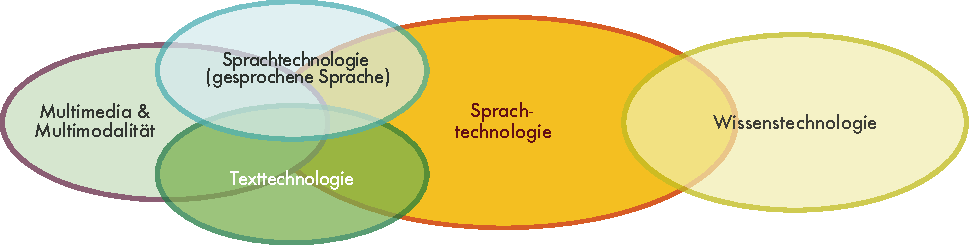
\includegraphics[width=\textwidth]{../_media/german/language_technologies}
  \caption{Sprachtechnologie im Kontext}
  \label{fig:ltincontext_de}
  \colorrule{grey3}{\textwidth}{1.5pt}
\end{figure*}

Toliau aptarsime pagrindines KT taikymo sritis, pavyzdžiui, kalbos taisyklingumo tikrinimą, paiešką internete, šnekamosios KT ir automatinį vertimą, kurios apima tokius technologijų pritaikymo būdus:

\begin{itemize}
\item  rašybos ir gramatikos tikrinimą;
\item pagalbą kuriant dokumentus;
\item kalbų mokymąsi;
\item  informacijos paiešką;
\item  informacijos išgavimą;
\item tekstų santraukų kūrimą;
\item atsakymus į klausimus;
\item šnekos atpažinimą; 
\item  šnekos sintezę.
\end{itemize}

KT tyrimo sritis yra gerai įsitvirtinusi ir įvadinės literatūros galima rasti vis daugiau. Susidomėjusiems skaitytojams siūlomos šios publikacijos:  \cite{carstensen-etal1, jurafsky-martin01, manning-schuetze1, lt-world1, lt-survey1}.

 Prieš aptardami išvardytas pritaikymo sritis, trumpai pakalbėkime apie tipinės KT sistemos architektūrą.  

\subsection{Kalbos technologijų taikymo architektūra}

Kalbos apdorojimo programinę įrangą paprastai sudaro keletas komponentų, atspindinčių skirtingus kalbos aspektus.  \ref{fig:textprocessingarch_de} paveiksle parodyta itin supaprastinta tipinės teksto apdorojimo sistemos struktūra. Pirmieji trys moduliai apdoroja įvedamo teksto struktūrą ir nustato pradinius semantikos duomenis:

\begin{figure*}[htb]
  \colorrule{grey3}{\textwidth}{1.5pt}
  \center
  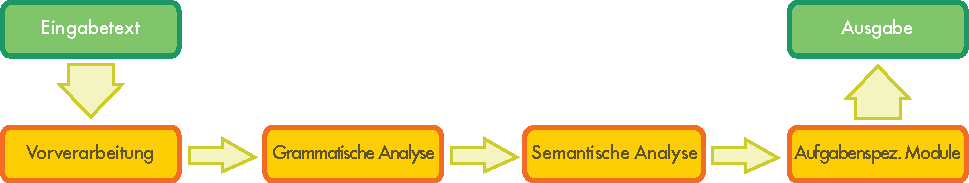
\includegraphics[width=\textwidth]{../_media/german/text_processing_app_architecture}
  \caption{Eine typische Architektur zur Verarbeitung von Texten}
  \label{fig:textprocessingarch_de}
  \colorrule{grey3}{\textwidth}{1.5pt}
\end{figure*}

\begin{enumerate}
\item Pirminis duomenų apdorojimas (angl. \textit{pre-processing}):  duomenys „išvalomi“, išanalizuojamas arba pašalinamas formatavimas, nustatoma įvesties kalba ir pan.
\item Gramatinė analizė: atliekama žodžių morfologinė analizė, nustatomos kalbos dalys ir pagrindinės žodžių formos, surandamas veiksmažodis, jo papildiniai, aplinkybės ir kitos kalbos dalys, nustatoma sakinio struktūra.
\item Semantinė analizė: nustatoma žodžio reikšmė (t. y. išanalizuojama apytikslė žodžių reikšmė tiriamame kontekste); išsprendžiamos anaforos (t. y. nustatoma, kurie įvardžiai sakinyje atitinka kuriuos daiktavardžius) ir posakių pakeitimo problemos; sakinio prasmė pateikiama kompiuteriui suvokiamu būdu.
\end{enumerate}

Išanalizavus tekstą, specialioms užduotims sukurti moduliai gali atlikti ir kitokius veiksmus, pavyzdžiui, sukurti teksto santrauką ar ieškoti informacijos duomenų bazėse.
 
Pristatę pagrindines sritis, kuriose taikomos KT, trumpai apžvelgsime dabartinę KT tyrimų ir švietimo būklę, jau įgyvendintas ir šiuo metu vykdomas mokslinių tyrimų programas. Po to pateiksime profesionalų atliktą pagrindinių KT įrankių ir išteklių įvertinimą įvairiais aspektais – prieinamumo, išbaigtumo, kokybės ir pan. Bendroji lietuvių kalbos KT būklė pateikiama 8 lentelėje.

\subsection{Pagrindinės taikymo sritys} 

Šiame skyriuje daugiausia dėmesio skirsime svarbiausiems KT įrankiams ir ištekliams, apžvelgsime KT padėtį Lietuvoje. Įrankius ir išteklius, kurių pavadinimai tekste pabraukti, galima rasti ir šio skyriaus pabaigoje pateiktoje 8 lentelėje. 

\subsubsection{Rašybos ir gramatikos tikrinimas}

Kam yra tekę naudotis teksto rašymo programa, pavyzdžiui, \textit{Microsoft Word}, žino, kad joje yra funkcija tikrinti, ar nėra rašybos klaidų. Ji klaidas randa, parodo ir siūlo taisymo variantus. Pirmosios rašybos klaidų taisymo programos palygindavo atrinktus žodžius su taisyklingos rašybos žodynu. Šiandien tokios programos yra kur kas sudėtingesnės. Naudodamos su konkrečia kalba susietus teksto analizės algoritmus, jos aptinka morfologines (pvz., daugiskaitos darybos klaidas) ir sintaksines (pvz., praleistus veiksmažodžius arba nesuderintus veiksnius ir tarinius, pvz., \textit{ji *rašyti laišką}) klaidas. Tačiau dauguma rašybos klaidų taisymo programų neras jokių klaidų tokiame tekste anglų kalba \cite{zar1}:

\begin{quote}
  I have a spelling checker,\\
  It came with my PC.\\
  It plane lee marks four my revue\\
  Miss steaks aye can knot sea.
\end{quote}

Tokiai analizei atlikti reikalinga arba ekspertų į programinę įrangą kruopščiai perkelta konkrečios kalbos gramatika, arba statistinis kalbos modelis. Šiuo atveju modelis apskaičiuoja tam tikro žodžio vartojimo kitų žodžių apsuptyje tikimybę. Statistinį kalbos modelį galima sukurti automatiškai, panaudojant didelį skaičių taisyklingų kalbos duomenų (tekstyną). Šie du metodai daugiausia buvo išplėtoti naudojant anglų kalbos duomenis. Taigi nė vieno metodo negalima lengvai pritaikyti lietuvių kalbai, kadangi lietuvių kalbos žodžių tvarka nėra fiksuota, o kaitybos sistema yra kur kas sudėtingesnė (nuo 2002 m. VDU mokslininkai nemažai dirbo su statistiniu lietuvių kalbos modeliu, įrankius galima nemokamai atsisiųsti \cite{airenas}).   

\boxtext{Kalbos taisyklingumo tikrinimo programos naudojamos ne tik rašant tekstus, jas galima pritaikyti ir dokumentų kūrimo pagalbinėse sistemose.}

Kalbos taisyklingumo tikrinimo programos naudojamos ne tik rašant tekstus, jas galima pritaikyti ir dokumentų kūrimo pagalbinėse sistemose (angl. \textit{authoring support systems}), t. y. programinėje terpėje, kurioje laikantis ypatingų standartų kuriami sudėtingų informacinių technologijų sistemų, sveikatos priežiūros, inžinerijos ir kitokių sričių vadovai bei kitokie dokumentai. Nuogąstaudamos, kad klientai pradės skųstis dėl to, jog produktas bus naudojamas ne taip, kaip reikia, o dėl nesuprantamų instrukcijų bus pateikta reikalavimų kompensuoti žalą, bendrovės vis daugiau dėmesio skiria techninės dokumentacijos kokybės gerinimui, tuo pat metu orientuodamosios į tarptautines rinkas (versdamos tekstus arba juos pritaikydamos konkrečiai kalbai). Pažanga, pasiekta apdorojant natūralią kalbą, paskatino plėtoti dokumentų kūrimo pagalbines sistemas. Šios sistemos padeda techninių dokumentų autoriui naudoti tos srities žodyną ir sakinių struktūras, atitinkančias srities taisykles, verslo terminiją.

\begin{figure*}[htb]
  \colorrule{grey3}{\textwidth}{1.5pt}
  \center
  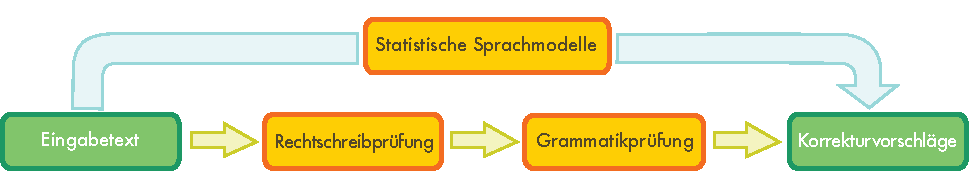
\includegraphics[width=\textwidth]{../_media/german/language_checking}
  \caption{Sprachüberprüfung (statistisch; regelbasiert)}
  \label{fig:langcheckingaarch_de}
  \colorrule{grey3}{\textwidth}{1.5pt}
\end{figure*}

Šioje srityje ką pasiūlyti turi vos keletas Lietuvos bendrovių. 1992–1994 m. UAB „Fotonija“ sukūrė rašybos tikrinimo programą \textit{Juodos Avys}, kuri buvo nuolat tobulinama. Automatinio rašybos tikrinimo metu veikia algoritmas, padedantis išvengti savaiminio pavardės ar pavadinimo pakeitimo į kitą. Atpažįstami neteiktini žodžiai ir siūloma juos keisti į tinkamus. Teikiami pasiūlymai dėl trūkstamų specifinių lietuviškų rašmenų, tokių kaip \textit{š}, \textit{ž},  \textit{ū}, \textit{ė} taisymo. Į tikrintuvę integruotas lietuviškų skiemenų rašymo su brūkšneliu įrankis.   

    UAB „Tilde IT“  lietuvių kalbos rašybos tikrinimo programą sukūrė 2001 m. Ši bendrovė tobulina rašybos tikrinimo programą ir kuria naują gramatikos tikrinimo programą, kuri analizuos sakinio struktūrą, atpažins praleistus arba nereikalingus kablelius ir kitokius skyrybos ženklus, tikrins, ar nėra sintaksės ir leksikos klaidų. Gramatikos tikrintuvė veiks ne tik su platforma \textit{Microsoft Office}, bet ir su platforma \textit{Open Office} ar internetinėmis programomis. Ji bus nesunkiai suderinama su kitomis programomis, kuriose naudojamos su kalba susijusios funkcijos (pvz., įmonės išteklių tvarkymo programomis, verslo sprendimais ir pan.). Naudotojai turės galimybę išbandyti naująją gramatikos klaidų taisymo programą 2012 metais.   

    Kalbos tikrinimo funkcija svarbi ne tik rašybos tikrinimo ir dokumentų kūrimo programose – ji reikalinga ir skaitmeninėje terpėje mokantis kalbų. Be to, kalbos tikrinimo įrankiai automatiškai taiso į paieškos sistemas įvedamas užklausas, teikia teisingų užklausų pasiūlymus – čia kaip pavyzdį galime paminėti sistemos  \textit{Google} įrankį \textit{Galbūt jūs norėjote ieškoti...}  (angl. \textit{Did you mean…}).

\subsubsection{Paieška internete }

 Paieška internete, vidaus tinkluose ar skaitmeninėse bibliotekose šiandien turbūt yra plačiausia, tačiau mažiausiai išplėtota KT pritaikymo sritis. Paieškos sistema \textit{Google}, kuri buvo pristatyta 1998 metais, šiuo metu apdoroja apie 80 proc. visų užklausų \cite{spi1}.  Sistemos \textit{Google} paieškos sąsaja ir langas, kuriame pateikiami rezultatai, ne itin pasikeitė palyginti su pirmąja sistemos versija. Tačiau dabartinė \textit{Google} versija turi rašybos klaidų taisymo ir esminių semantinės paieškos funkcijų, analizuojančių užklausos terminų kontekstinę reikšmę ir galinčių padidinti paieškos tikslumą \cite{pc1}.  Sistemos \textit{Google} sėkmė rodo, kad gausybė sukauptų duomenų ir veiksmingi rodyklių sudarymo įrankiai gali padėti pasiekti neblogų rezultatų taikant statistinį metodą. 

\begin{figure*}[htb]
  \colorrule{grey3}{\textwidth}{1.5pt}
  \center
  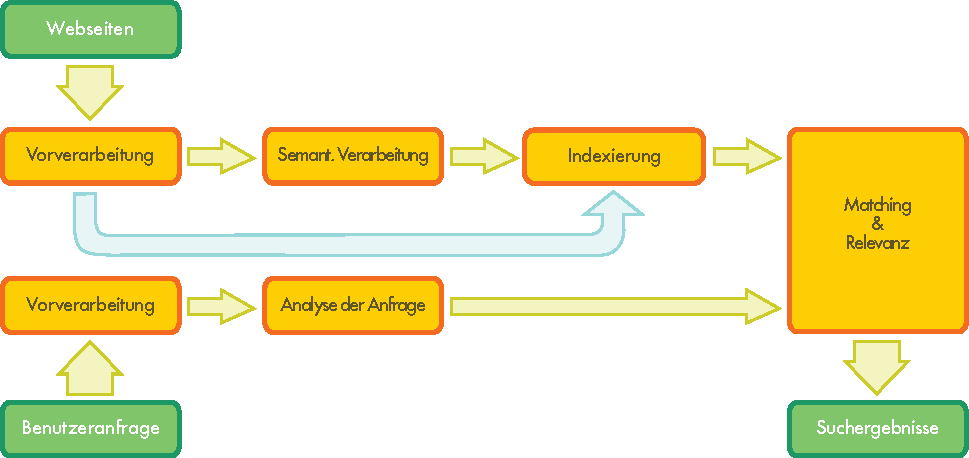
\includegraphics[width=\textwidth]{../_media/german/web_search_architecture}
  \caption{Websuche}
  \label{fig:websearcharch_de}
  \colorrule{grey3}{\textwidth}{1.5pt}
\end{figure*}

 Norint apdoroti įmantresnes informacijos užklausas, būtinos nuodugnesnės lingvistinės tekstų interpretavimo žinios. Eksperimentai su leksikos ištekliais, pavyzdžiui, kompiuteriui suprantamais tezaurais ar ontologiniais kalbų ištekliais (pvz., \textit{WordNet} anglų kalba ar \textit{GermaNet} vokiečių kalba), parodė, kad vartojant pirminių terminų sinonimus, tokius kaip \textit{Atomkraft} [atominė energija], \textit{Kernenergie} [atominė galia] ir \textit{Nuklearenergie} [branduolinė energija], ar net ne taip glaudžiai tarpusavyje susijusius terminus, randama vis daugiau internetinių puslapių. 

Naujosios kartos paieškos sistemos turės būti grindžiamos kur kas pažangesnėmis KT, ypač turint galvoje užklausas, kurias sudaro klausimas ar kitoks sakinys, o ne keli esminiai žodžiai. Apdorodama užklausą „Pateikite man sąrašą bendrovių, kurias per pastaruosius penkerius metus įsigijo kitos bendrovės“, KT sistema turi išanalizuoti sakinį sintaksės ir semantikos požiūriu bei pateikti rodyklę, kuri leistų operatyviai rasti reikiamus dokumentus. Norint pateikti patenkinamą atsakymą, prireiks išnagrinėti sakinio sintaksę nustatant, kad naudotojas prašo pateikti sąrašą bendrovių, kurios buvo įsigytos, o ne kurios įsigijo kitų bendrovių. Apdorodama posakį \textit{pastaruosius penkerius metus}, sistema turi nustatyti reikiamus metus. Be to, užklausą reikia palyginti su gausybe nesusistemintų duomenų, ieškant naudotojo pageidaujamos informacijos. Šis procesas vadinamas \textit{informacijos paieška}, jį sudaro tam tikrų dokumentų paieška ir vertinimas. Rengdama bendrovių sąrašą sistema dar turi atpažinti ir konkrečią žodžių seką dokumente, pavyzdžiui, bendrovės pavadinimą – toks procesas vadinamas \textit{įvardytų subjektų atpažinimu}.  

\boxtext{Naujosios kartos paieškos sistemos turės būti grindžiamos kur kas pažangesnėmis kalbos technologijomis.}

Dar sunkesnis darbas – derinti užklausą, pateiktą viena kalba, ir dokumentus, skelbiamus kita kalba. Informacijos skirtingomis kalbomis paieška reiškia, kad reikės automatiškai išversti užklausą į visas įmanomas informacijos šaltinių kalbas, o po to rezultatus vėl išversti į užklausos kalbą.   

    Dabar duomenys vis dažniau pateikiami ne tekstiniais formatais, tad didėja daugialypėje terpėje – paveikslėliuose, garso ir vaizdo bylose – esančios informacijos paieškos poreikis. Garso ir vaizdo bylų informaciją kalbos atpažinimo modulis turi paversti tekstu (arba fonetine transkripcija), kuris galės būti palygintas su naudotojo užklausa.   

    Lietuvių kalbos pritaikymui šios technologijos tik pradedamos intensyviau plėtoti. Su šia sritimi susijusius tyrimus ir projektus vykdo Vytauto Didžiojo universitetas (projektą „Informacijos valdymo semantinė sistema“ pagal Ekonomikos augimo veiksmų programą remia Europos Sąjungos struktūriniai fondai), Vilniaus universiteto Matematikos ir informatikos institutas, Kauno technologijos universitetas. Semantinių tinklų, ontologijų kūrimo, žinių ir dokumentų tvarkymo srityje pradeda dirbti kai kurios KT srityje dirbančios verslo kompanijos, pavyzdžiui, UAB „Sintagma“, sukūrusi dokumentų tvarkymo sistemą \textit{Avilys}. UAB „Tilde IT“ nuo 2008 metų plėtoja semantinių sistemų srities projektus ir šiuo metu įgyvendina lingvistinio semantinio tinklo kūrimo projektą \textit{SemTi}, taip pat dalyvauja tarptautiniame SOLIM projekte (angl. \textit{Spatial Ontology Language for Multimedia Information Modeling}). Atskirų sričių, pavyzdžiui, bibliotekų, mokslo, ontologijos pradedamos intensyviau diegti tik pastaruoju metu.   

    Kol kas šioje srityje pastangos fragmentiškos ir didesnio proveržio tikimasi iš Lietuvos Respublikos Vyriausybės inicijuotos Lietuvių kalbos informacinėje visuomenėje 2009–2013 metų programos, pagal kurią numatoma sukurti priemones, pritaikytas teikti sintaksinės-semantinės analizės paslaugą, analizuoti lietuviškų interneto svetainių turinį, atlikti pagal jį paiešką ir pan.
  
\subsubsection{Šnekamosios kalbos technologijos}

Šnekamosios KT taikomos norint sukurti sąsajas, leisiančias naudotojams bendrauti su kompiuteriu balsu, o ne naudojantis grafiniu ekranu, klaviatūra ir pele. Šiandien naudotojo balso sąsajos (angl.\textit{voice user interfaces}, VUI) paprastai naudojamos teikiant iš dalies arba visiškai automatizuotas telefono paslaugas klientams, darbuotojams ar partneriams. Naudotojo balso sąsajos yra itin aktualios bankininkystėje, tiekimo sistemose, viešajame transporte ir telekomunikacijose. Kitos sritys, kuriose taikomos šnekamosios KT, yra automobilių navigacijos sistemų sąsajos ir šnekamosios kalbos sąsaja vietoje išmaniųjų telefonų grafinių arba liečiamųjų ekranų sąsajų.

\boxtext{Šnekamosios kalbos technologijos taikomos norint sukurti sąsajas, leisiančias naudotojams bendrauti su kompiuteriu balsu, o ne naudojantis ekranu, klaviatūra ir pele.}

\begin{figure*}[htb]
  \colorrule{grey3}{\textwidth}{1.5pt}
  \center 
  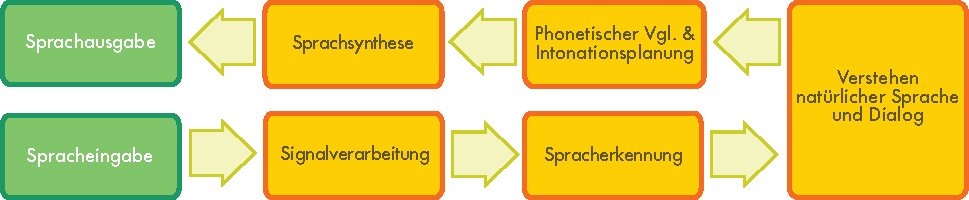
\includegraphics[width=\textwidth]{../_media/german/simple_speech-based_dialogue_architecture}
  \caption{Sprachdialogsystem}
  \label{fig:dialoguearch_de}
  \colorrule{grey3}{\textwidth}{1.5pt}
\end{figure*}

Šnekamajai kalbai skirtos keturios technologijos:

\begin{enumerate}
\item \textbf{Automatinis kalbos atpažinimas} (angl. \textit{automatic speech recognition}, ASR) nustato, kokius žodžius sudaro naudotojo ištarta garsų seka.
\item Natūralios kalbos suvokimo technologija analizuoja naudotojo ištartos frazės morfologinę ir sintaksinę struktūrą ir ją interpretuoja pagal atitinkamos sistemos taisykles.
\item  Dialogo valdymo technologija nustato, kokių veiksmų imtis atsižvelgiant į naudotojo įvestus duomenis ir sistemos funkcijas.    
\item \textbf{Kalbos sintezė} (rašytinio teksto pavertimo šnekamąja kalba, angl. \textit{text-to-speech}, TTS) sistemos atsakymą naudotojui transformuoja į garsą.
\end{enumerate}

Vienas iš didžiausių keblumų, su kuriais susiduria automatinio kalbos atpažinimo sistemos, yra tikslus naudotojo ištartų žodžių atpažinimas. Reikia apriboti galimų naudotojo pasakymų skaičių iki tam tikro esminių žodžių sąrašo arba rankiniu būdu sukurti kalbos modelius, apimančius daugybę natūralios kalbos pasakymų. „Mokant“   kompiuterines programas, kalbos modelius galima kurti ir automatiškai, pasitelkiant šnekamosios kalbos garsynus – gausias kalbos garsinių bylų ir tekstų transkripcijų rinkinius. Apribojus ištariamų pasakymų skaičių, žmonės verčiami naudotis balso sąsajomis itin tiksliai ir dėl tos priežasties tokios sistemos gali tapti nepatogios naudotojams. Kita vertus, sukurti, priderinti ir prižiūrėti turiningus bei išsamius kalbų modelius galima tik labai padidinus išlaidas. Kalbų modeliais pagrįstos ir naudotojui galimybę lanksčiau išreikšti pageidavimus suteikiančios (vartojant posakį \textit{Kuo galiu jums padėti?}) naudotojo balso sąsajos dažniausiai būna automatinės ir gerokai priimtinesnės. 

Bendrovės, kurdamos naudotojo balso sąsajų išvedimą, linkusios naudoti profesionalių diktorių iš anksto įrašytas frazes. Statinių pasakymų atveju, kai žodžiai nepriklauso nuo konkretaus konteksto ar naudotojo asmeninių duomenų, tokia sistema gali pasirodyti itin patraukli. Tačiau dinamiškesnis turinys gali nukentėti dėl nenatūralios intonacijos, kadangi atskiri garsinių bylų segmentai būna tiesiog susieti vienas su kitu. Dabartinės kalbos sintezės sistemos vis tobulėja (nors jas vis dar reikia gerinti), jos sugeba atkurti natūraliai skambančią dinamišką kalbą.   

    Per pastarąjį dešimtmetį buvo gerokai standartizuoti rinkoje turimų šnekamosios KT sąsajų įvairūs technologiniai komponentai. Be to, kalbos atpažinimo bei kalbos sintezės rinkos ir toliau intensyviai konsolidavosi. Dvidešimties didžiųjų šalių G20 (ekonomiškai stabilių šalių, pasižyminčių dideliu gyventojų skaičiumi) rinkose vyravo vos penki pasauliniai dalyviai, iš kurių Europoje aktyviausios buvo bendrovės „Nuance“ (JAV) ir „Loquendo“ (Italija). 2011 metais bendrovė „Nuance“ paskelbė įsigijusi bendrovę „Loquendo“ – tai yra dar vienas rinkos konsolidacijos žingsnis.   

    Lietuvoje šnekamosios KT moksliniai tyrimai nuo 1980 metų atliekami Kauno technologijos universitete (KTU). Jau daugelį metų šie darbai dirbami Vilniaus universiteto Matematikos ir informatikos institute, taip pat tyrimai atliekami Vytauto Didžiojo universitete.   

    Kauno technologijos universiteto Kalbos tyrimų laboratorijoje automatinio kalbos atpažinimo tyrimai tęsiami nuo 1980 m. Laboratorija yra sukūrusi komandų ir skaitmeninių sekų garsyną. Kuriami lietuviški kompiuteriniai dialogai, sukauptas ir tobulinamas lietuvių šnekamosios kalbos garsynas LTDIGITS. Jį sudaro ištisinės skaičių sekos ir lietuviški žodžiai kompiuteriui valdyti. Lietuvių kalbos ženklų tyrimai atliekami ir Vilniaus universiteto Matematikos ir informatikos institute, sukaupusiame Lietuvos radijo žinių garsyną LRNO. Vytauto Didžiojo universitete sukauptas universalus šnekamosios lietuvių kalbos garsynas (čia kaupiama ir mažesnės apimties specialiųjų tekstynų, skirtų kalboms mokytis, pavyzdžiui, jaunuolių sakytinės kalbos tekstynas SACODEYL ir pan.). Vyksta ir šnekamosios lietuvių kalbos automatinio skaidymo tyrimai, kuriama šnekamosios lietuvių kalbos automatinė transkripcija.   

    Nors tyrimai ir toliau vyksta siekiant gerinti kokybę, automatinio kalbos atpažinimo programinė įranga šiuo metu sėkmingai taikoma teisėsaugoje, telefonijoje, švietime, transporte, internete ir kitur.   

    Vilniaus universitete atlikti šnekamosios kalbos sintezės ir tokių sistemų pritaikymo akliesiems ir silpnaregiams tyrimai. Lietuviškos balso sintezės programos \textit{Aistis} svarbiausi komponentai yra šie: a) automatinis lietuviškų žodžių skaidymas skiemenimis; b) žodžių lietuvių kalba parašytame tekste automatinis kirčiavimas; c) automatinis lietuviškų tekstų transkribavimas; d) fonetinių vienetų bazė; e) lietuviškų tekstų pavertimo šnekamąja kalba kokybės įvertinimas. Šia programa lengva naudotis, ji skirta specialiųjų poreikių, pavyzdžiui, fizinę negalią turintiems naudotojams ar senyvo amžiaus žmonėms. Balso sintezatorių MBROLA galima lengvai rasti internete, jis yra pagrįstas Vilniaus universitete Alekso Girdenio ir Pijaus Kasparaičio sukurta fonetinių vienetų baze.   

    Programos \textit{Aistis}  komponentai buvo pritaikyti kuriant lietuvių kalbos sintezatorių \textit{WinTalker Voice}, kuriame buvo įdiegti du balsai: \textit{Gintaras}  ir \textit{Aistis2}. Šią programą Lietuvos aklųjų ir silpnaregių draugijos užsakymu išleido čekų bendrovė „Rosasoft“. Derėtų paminėti, kad Lietuvoje yra apie 7 tūkst. žmonių, turinčių specialiųjų poreikių, o 2010 m. kovo 1 d. duomenimis, visoje Lietuvoje kompiuteriu naudojosi 258 aklieji ir silpnaregiai. Dar vieną nemokamą balso sintezatorių sukūrė UAB „Etalinkas“.  Šis sintezatorius yra pritaikytas dirbti su operacinėmis sistemomis \textit{Windows} ir \textit{Linux}.

Vytauto Didžiojo universitete šnekos atpažinimui tekstyno pagrindu sukurti statistiniai lietuvių kalbos modeliai, ištisinės šnekos atpažintuvo prototipas, apimantis daugiau nei 1 mln. žodžių formų, automatinio kirčiavimo programa su homografų vienareikšminimu, prieinama internete, bei lietuvių kalbos garsų trukmių modeliai.

Vis labiau populiarėjantys išmanieji telefonai, kaip nauja bendravimo su naudotojais priemonė greta fiksuotųjų telefonų, interneto ir elektroninio pašto, ateityje lems didžiulius pokyčius. Tai turės įtakos ir šnekamosios KT taikymui. Ilgainiui telefoninės naudotojo balso sąsajos sustiprės, o šnekamoji kalba taps naudotojams dar svarbesne ir patogesne priemone duomenims į sumaniuosius telefonus įvesti. Šiuos pokyčius skatins vis tikslesnis nuo kalbėtojo nepriklausantis kalbos atpažinimas, panaudojant šnekos diktavimo paslaugas. Tokios centralizuotos paslaugos jau dabar yra siūlomos išmaniųjų telefonų naudotojams.

\subsubsection{Automatinis vertimas}

 Sumanymas pritaikyti kompiuterius versti iš vienos kalbos į kitą kilo 1946 m., o šeštajame ir vėliau devintajame praėjusio amžiaus dešimtmetyje šiems tyrimams buvo skirta nemažai lėšų. Tačiau ir šiuo metu automatinis vertimas vis dar negali tenkinti visuotinio vertimo poreikių.

\boxtext{Paprasčiausios automatinio vertimo programos tiesiog pakeičia vienos kalbos žodžius kitos kalbos žodžiais.}

Paprasčiausias automatinio vertimo būdas – automatiškai pakeisti vienos kalbos žodžius kitos kalbos žodžiais. Šis būdas gali būti naudingas tose srityse, kurių kalba yra labai standartizuota ir šabloniška, pavyzdžiui, rengiant orų prognozes. Tačiau norint gauti kokybišką ne tokių standartinių tekstų vertimą, didesni teksto vienetai (frazės, sakiniai ar net visos pastraipos) turi būti sugretinti su jų artimiausiais atitikmenimis ta kalba, į kurią verčiama. Sunkiausia įveikti žmonių kalbos polisemiją, kuris kelia problemų skirtingiems kalbos lygmenims, pavyzdžiui, nustatant daugiareikšmių žodžių leksinę reikšmę (\textit{jaguaras} gali būti ir automobilio markė, ir gyvūnas) arba linksnį ar reikiamą formą sintaksinėse konstrukcijose, pavyzdžiui:

 \textit{I was happy to read a book.\\
      {[}Aš buvau laimingas:{}\\
      {}(a) perskaitęs knygą.{}\\
      {}(b) skaitydamas knygą.{}\\
      {}(c) galėdamas perskaityti knygą.{]} }     

Vienas iš būdų sukurti automatinio vertimo sistemą – pasinaudoti kalbos taisyklėmis. Verčiant iš vienos kalbos į jai giminingą kalbą, kaip jau minėta, galima būtų tiesiog pakeisti žodžius, tačiau taisyklėmis pagrįstos (arba į lingvistines žinias orientuotos) sistemos dažniausiai analizuoja įvedamą tekstą ir sukuria jo tarpinį simbolinį pavidalą, pagal kurį gali būti sukurtas išverstasis tekstas. Tokių metodų sėkmė itin priklauso nuo galimybės turėti išsamius žodynus, kuriuose pateikiama morfologinė, sintaksinė ir semantinė informacija, bei gausius gramatikos taisyklių rinkinius, parengtus profesionalių kalbininkų. Tai labai ilgas ir, žinoma, labai daug kainuojantis darbas.

\begin{figure*}[htb]
  \colorrule{grey3}{\textwidth}{1.5pt}
  \center
  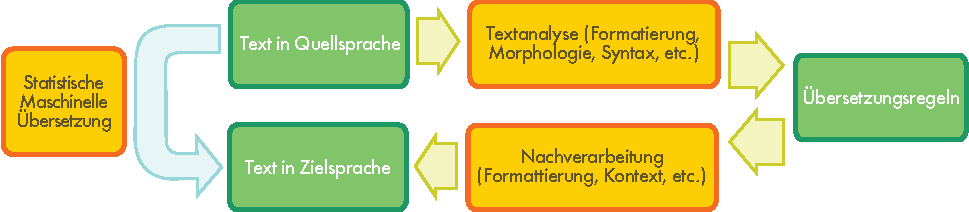
\includegraphics[width=\textwidth]{../_media/german/machine_translation}
  \caption{Maschinelle Übersetzung (statistisch; regelbasiert)}
  \label{fig:mtarch_de}
  \colorrule{grey3}{\textwidth}{1.5pt}
\end{figure*}

 Praėjusio amžiaus devintojo dešimtmečio pabaigoje, pradėjus kurti galingesnius kompiuterius ir jiems atpigus, imta labiau domėtis automatinio vertimo statistiniais modeliais. Statistiniai modeliai išplėtoti analizuojant dvikalbius tekstynus, pavyzdžiui, lygiagretųjį tekstyną \textit{Europarl}, kuriame pateikiama Europos Parlamento posėdžių medžiaga vienuolika Europos kalbų. Turėdamos pakankamai duomenų, statistinės automatinio vertimo sistemos apdoroja lygiagrečias tekstų skirtingomis kalbomis versijas ir randa galimus žodžių modelius – dėl to jos tinka apytiksliams vertimams iš vienos kalbos į kitą. Tačiau, kitaip nei taisyklėmis pagrįstos sistemos, statistinės (arba duomenimis pagrįstos) automatinio vertimo sistemos dažnai pateikia gramatiškai netaisyklingų tekstų. Duomenimis pagrįstos automatinio vertimo sistemos yra pranašesnės, kadangi reikia mažiau žmogaus indėlio ir pastangų, be to, tokios sistemos gali atsižvelgti į tam tikras kalbos ypatybes (pvz., idiomas), kurių kalbos žiniomis pagrįstos sistemos gali ir nepastebėti.    

Ir taisyklėmis, ir duomenimis pagrįstų automatinio vertimo sistemų pranašumai ir trūkumai paprastai kompensuoja vieni kitus, todėl šiuo metu tyrėjai daugiausia dėmesio skiria hibridiniams metodams, susiejantiems šias dvi technologijas. Vienas toks metodas yra pagrįstas ir į taisykles, ir į duomenis orientuotomis sistemomis, be to, turi modulį, sugebantį pasirinkti, kuris būdas geriausiai tinka konkrečiam sakiniui išversti. Tačiau sakinių, ilgesnių nei, tarkim, 12 žodžių, vertimo rezultatai tikrai nebus tobuli. Tokiu atveju geriausiai pasirinkti pagal prasmę tinkamiausias kiekvieno vertimo varianto dalis. Šis procesas gali būti gana sudėtingas, kadangi alternatyvių variantų sutampančios dalys ne visuomet yra aiškios, jas reikia papildomai sugretinti. 

\boxtext{Automatinis vertimas iš lietuvių kalbos – itin didelis iššūkis.} 

Automatinis vertimas iš lietuvių kalbos – itin didelis iššūkis. Laisva žodžių tvarka ir veiksmažodinės konstrukcijos sunkina analizę, o dėl linksniuočių įvairovės sunku parinkti reikiamos giminės ir linksnio žodžius.   

    Mažiau vartojamų kalbų, tokių kaip baltų kalbos, automatinio vertimo tyrimų įrankiai, kaip ir apskritai pačios KT, nėra labai gerai išplėtotos. Lietuvoje atlikta keletas su automatiniu vertimu susijusių darbų. Internete šiuo metu galima rasti tris vertimo įrankius: projektą WIFTA \cite{vertvdu},  sistemą \textit{Google translator} ir \textit{Vertimo vedlį} \cite{mvlab}. Pirmoji sistema buvo sukurta 2008 metais drauge su Rusijos bendrove „ProMT“, jos pagrindu tapo taisyklėmis pagrįsta technologija. Ši sistema verčia atsižvelgdama į teksto morfologines, sintaksines ir semantines savybes. Projektas sėkmingai baigtas ir nuo 2008 m. prieinama internetu: http://vertimas.vdu.lt. Į ją kreipiamasi 127 mln. kartų per metus ir ja naudojasi maždaug 1 mln. unikalių vartotojų per metus. Registruotiems vartotojams suteikta galimybė naudotis kompiuterinių terminų ir verslo žodynais.

   Atvirai internetu prieinamas Vytauto Didžiojo universitete sukauptas dabartinės rašomosios lietuvių kalbos tekstynas, turintis apie 140 mln. žodžių \cite{tekstynas}.  Be to, sudaromas lygiagretusis lietuvių kalbos ir kitų (anglų, vokiečių, čekų) kalbų tekstynas, rengiama ir daugiau specialioms sritims skirtų tekstynų (pavyzdžiui, Vilniaus universitete sukauptas lietuvių mokslo kalbos tekstynas \textit{CorALit} \cite{coralit}). Deja, dabartinio lietuvių kalbos tekstyno modernioms lietuvių KT (informacijos paieškos, automatinio vertimo ir kitoms sistemoms) nebepakanka. Esamiesiems ir būsimiesiems tekstynams reikia bendros lietuvių kalbai pritaikytos programinės įrangos, kuri leistų kuo geriau išnaudoti turimus kalbos išteklius ir iš jų gaunamus skaitmeninius aprašus. Viena iš privalomų sąlygų klasikinėms automatinio vertimo sistemoms yra galimybė naudotis didžiuliu lygiagrečiuoju tekstynu, iš kurio kompiuteris gali mokytis. Didelių lygiagrečiųjų tekstynų trūkumas yra pagrindinė priežastis, dėl kurios Baltijos šalys tik dabar pradeda eksperimentuoti su automatinio vertimo sistemomis.   

    Sistemos \textit{Google} automatinio vertimo programinė įranga yra pagrįsta statistiniu metodu, o jos galimybės apima apie 30 kalbų, taip pat ir lietuvių.   

   \textit{Vertimo vedlys}  – tai eksperimentinis automatinio vertimo įrankis, kurį sukūrė Lietuvių kalbos institutas kartu su UAB „Tilde IT“. Bandomoji versija verčia iš lietuvių kalbos į anglų kalbą. Automatizuota vertimo priemonė analizuoja sakinių struktūrą ir automatiškai siūlo sakinio, jo dalies ar atskirų žodžių vertimą. Ji yra pagrįsta statistine vertimo technologija ir sistemomis \textit{Giza++}  ir \textit{Moses}. Bendrovė „Tilde IT“ kuria lietuvių–anglų kalbų automatinio vertimo sistemą, integruodama statistinius ir taisyklėmis pagrįstus automatinio vertimo metodus, diegdama novatoriškas iš keleto žodžių sudarytų frazių apdorojimo funkcijas. Vertimo tikslumas – 30 proc., o sistema yra nuolat tobulinama. Bendrovės „Tilde IT“ automatinio vertimo sistema naudojama ne tik tekstams versti, bet ir ieškoti informacijos skirtingų kalbų šaltiniuose.   

    Tikimasi, kad automatinio vertimo sistemų kokybę dar galima labai pagerinti. Paprastai šioje srityje susiduriama su tokiomis problemomis, kaip galimybės pritaikyti kalbos išteklius tam tikrai sričiai ar naudotojo poreikiams, sukurti jų darbinę sąveiką su terminijos bazėmis ir vertimų atmintimi. Be to, dauguma šiuo metu egzistuojančių sistemų yra pritaikytos anglų kalbai, galimybės versti iš lietuvių kalbos į kitokias kalbas ir iš kitokių kalbų į lietuvių kalbą yra ribotos, dėl to stringa bendras vertimų srautas, taip pat naudotojai privalo mokytis skirtingose sistemose taikomų skirtingų priemonių žodynams koduoti.   

    Vertinimas padeda palyginti automatinio vertimo sistemų kokybę, skirtingus metodus ir šių sistemų būklę skirtingose kalbų porose. Apačioje pateiktoje lentelėje, kuri sudaryta Europos Komisijos projekto „Euromatrix+“ metu, parodyti dvidešimt dviejų iš dvidešimt trijų oficialiųjų Europos Sąjungos kalbų (airių kalba į lyginimą nebuvo įtraukta) lyginimo rezultatai. Rezultatai išdėstyti eilės tvarka remiantis įvertinimo skale BLEU, pagal kurią už geresnį vertimą skiriamas aukštesnis balas \cite{bleu1}.  Vertėjas žmogus gautų apie 80 balų įvertinimą.   

    Geriausi rezultatai (pažymėti žalia ir mėlyna spalva) buvo pasiekti verčiant kalbas, kurios yra išsamiai ištirtos pagal koordinuotas programas ir turinčios daugybę lygiagrečiųjų tekstynų (pvz., anglų, prancūzų, olandų, ispanų ir vokiečių kalbos). Kalbos, kurių įvertinimo rezultatai prastesni, pažymėtos raudona spalva. Šios kalbos arba nepakankamai ištirtos, arba jų struktūra smarkiai skiriasi nuo kitų kalbų (pvz., vengrų, maltiečių ir suomių kalbos).

\begin{figure*}[htbp]
  \centering
  \setlength{\tabcolsep}{0.17em}
  \small
  \begin{tabular}{>{\columncolor{corange1}}cccccccccccccccccccccccc}
    & \multicolumn{22}{>{\columncolor{corange1}}c}{Zielsprache -- \textcolor{grey1}{Target language}}\\\addlinespace[{-.009cm}]
    \rowcolor{corange1}  & EN & BG & DE & CS & DA & EL & ES & ET & FI & FR & HU & IT & LT & LV & MT & NL & PL & PT & RO & SK & SL & SV\\
    EN & -- & \textcolor{blue}{40.5} & \textcolor{blue}{46.8} & \textcolor{green2}{52.6} & \textcolor{green2}{50.0} & \textcolor{blue}{41.0} & \textcolor{green2}{55.2} & \textcolor{purple}{34.8} & \textcolor{purple}{38.6} & \textcolor{green2}{50.1} & \textcolor{purple}{37.2} & \textcolor{green2}{50.4} & \textcolor{purple}{39.6} & \textcolor{blue}{43.4} & \textcolor{purple}{39.8} & \textcolor{green2}{52.3} & \textcolor{blue}{49.2} & \textcolor{green2}{55.0} & \textcolor{blue}{49.0} & \textcolor{blue}{44.7} & \textcolor{green2}{50.7} & \textcolor{green2}{52.0}\\
    BG & \textcolor{green}{61.3} & -- & \textcolor{purple}{38.7} & \textcolor{purple}{39.4} & \textcolor{purple}{39.6} & \textcolor{purple}{34.5} & \textcolor{blue}{46.9} & \textcolor{red3}{25.5} & \textcolor{red3}{26.7} & \textcolor{blue}{42.4} & \textcolor{red3}{22.0} & \textcolor{blue}{43.5} & \textcolor{red3}{29.3} & \textcolor{red3}{29.1} & \textcolor{red3}{25.9} & \textcolor{blue}{44.9} & \textcolor{purple}{35.1} & \textcolor{blue}{45.9} & \textcolor{purple}{36.8} & \textcolor{purple}{34.1} & \textcolor{purple}{34.1} & \textcolor{purple}{39.9}\\
    DE & \textcolor{green2}{53.6} & \textcolor{red3}{26.3} & -- & \textcolor{purple}{35.4} & \textcolor{blue}{43.1} & \textcolor{purple}{32.8} & \textcolor{blue}{47.1} & \textcolor{red3}{26.7} & \textcolor{red3}{29.5} & \textcolor{purple}{39.4} & \textcolor{red3}{27.6} & \textcolor{blue}{42.7} & \textcolor{red3}{27.6} & \textcolor{purple}{30.3} & \textcolor{red2}{19.8} & \textcolor{green2}{50.2} & \textcolor{purple}{30.2} & \textcolor{blue}{44.1} & \textcolor{purple}{30.7} & \textcolor{red3}{29.4} & \textcolor{purple}{31.4} & \textcolor{blue}{41.2}\\
    CS & \textcolor{green2}{58.4} & \textcolor{purple}{32.0} & \textcolor{blue}{42.6} & -- & \textcolor{blue}{43.6} & \textcolor{purple}{34.6} & \textcolor{blue}{48.9} & \textcolor{purple}{30.7} & \textcolor{purple}{30.5} & \textcolor{blue}{41.6} & \textcolor{red3}{27.4} & \textcolor{blue}{44.3} & \textcolor{purple}{34.5} & \textcolor{purple}{35.8} & \textcolor{red3}{26.3} & \textcolor{blue}{46.5} & \textcolor{purple}{39.2} & \textcolor{blue}{45.7} & \textcolor{purple}{36.5} & \textcolor{blue}{43.6} & \textcolor{blue}{41.3} & \textcolor{blue}{42.9}\\
    DA & \textcolor{green2}{57.6} & \textcolor{red3}{28.7} & \textcolor{blue}{44.1} & \textcolor{purple}{35.7} & -- & \textcolor{purple}{34.3} & \textcolor{blue}{47.5} & \textcolor{red3}{27.8} & \textcolor{purple}{31.6} & \textcolor{blue}{41.3} & \textcolor{red3}{24.2} & \textcolor{blue}{43.8} & \textcolor{red3}{29.7} & \textcolor{purple}{32.9} & \textcolor{red3}{21.1} & \textcolor{blue}{48.5} & \textcolor{purple}{34.3} & \textcolor{blue}{45.4} & \textcolor{purple}{33.9} & \textcolor{purple}{33.0} & \textcolor{purple}{36.2} & \textcolor{blue}{47.2}\\
    EL & \textcolor{green2}{59.5} & \textcolor{purple}{32.4} & \textcolor{blue}{43.1} & \textcolor{purple}{37.7} & \textcolor{blue}{44.5} & -- & \textcolor{green2}{54.0} & \textcolor{red3}{26.5} & \textcolor{red3}{29.0} & \textcolor{blue}{48.3} & \textcolor{red3}{23.7} & \textcolor{blue}{49.6} & \textcolor{red3}{29.0} & \textcolor{purple}{32.6} & \textcolor{red3}{23.8} & \textcolor{blue}{48.9} & \textcolor{purple}{34.2} & \textcolor{green2}{52.5} & \textcolor{purple}{37.2} & \textcolor{purple}{33.1} & \textcolor{purple}{36.3} & \textcolor{blue}{43.3}\\
    ES & \textcolor{green}{60.0} & \textcolor{purple}{31.1} & \textcolor{blue}{42.7} & \textcolor{purple}{37.5} & \textcolor{blue}{44.4} & \textcolor{purple}{39.4} & -- & \textcolor{red3}{25.4} & \textcolor{red3}{28.5} & \textcolor{green2}{51.3} & \textcolor{red3}{24.0} & \textcolor{green2}{51.7} & \textcolor{red3}{26.8} & \textcolor{purple}{30.5} & \textcolor{red3}{24.6} & \textcolor{blue}{48.8} & \textcolor{purple}{33.9} & \textcolor{green2}{57.3} & \textcolor{purple}{38.1} & \textcolor{purple}{31.7} & \textcolor{purple}{33.9} & \textcolor{blue}{43.7}\\
    ET & \textcolor{green2}{52.0} & \textcolor{red3}{24.6} & \textcolor{purple}{37.3} & \textcolor{purple}{35.2} & \textcolor{purple}{37.8} & \textcolor{red3}{28.2} & \textcolor{blue}{40.4} & -- & \textcolor{purple}{37.7} & \textcolor{purple}{33.4} & \textcolor{purple}{30.9} & \textcolor{purple}{37.0} & \textcolor{purple}{35.0} & \textcolor{purple}{36.9} & \textcolor{red3}{20.5} & \textcolor{blue}{41.3} & \textcolor{purple}{32.0} & \textcolor{purple}{37.8} & \textcolor{red3}{28.0} & \textcolor{purple}{30.6} & \textcolor{purple}{32.9} & \textcolor{purple}{37.3}\\
    FI & \textcolor{blue}{49.3} & \textcolor{red3}{23.2} & \textcolor{purple}{36.0} & \textcolor{purple}{32.0} & \textcolor{purple}{37.9} & \textcolor{red3}{27.2} & \textcolor{purple}{39.7} & \textcolor{purple}{34.9} & -- & \textcolor{red3}{29.5} & \textcolor{red3}{27.2} & \textcolor{purple}{36.6} & \textcolor{purple}{30.5} & \textcolor{purple}{32.5} & \textcolor{red2}{19.4} & \textcolor{blue}{40.6} & \textcolor{red3}{28.8} & \textcolor{purple}{37.5} & \textcolor{red3}{26.5} & \textcolor{red3}{27.3} & \textcolor{red3}{28.2} & \textcolor{purple}{37.6}\\
    FR & \textcolor{green}{64.0} & \textcolor{purple}{34.5} & \textcolor{blue}{45.1} & \textcolor{purple}{39.5} & \textcolor{blue}{47.4} & \textcolor{blue}{42.8} & \textcolor{green}{60.9} & \textcolor{red3}{26.7} & \textcolor{purple}{30.0} & -- & \textcolor{red3}{25.5} & \textcolor{green2}{56.1} & \textcolor{red3}{28.3} & \textcolor{purple}{31.9} & \textcolor{red3}{25.3} & \textcolor{green2}{51.6} & \textcolor{purple}{35.7} & \textcolor{green}{61.0} & \textcolor{blue}{43.8} & \textcolor{purple}{33.1} & \textcolor{purple}{35.6} & \textcolor{blue}{45.8}\\
    HU & \textcolor{blue}{48.0} & \textcolor{red3}{24.7} & \textcolor{purple}{34.3} & \textcolor{purple}{30.0} & \textcolor{purple}{33.0} & \textcolor{red3}{25.5} & \textcolor{purple}{34.1} & \textcolor{red3}{29.6} & \textcolor{red3}{29.4} & \textcolor{purple}{30.7} & -- & \textcolor{purple}{33.5} & \textcolor{red3}{29.6} & \textcolor{purple}{31.9} & \textcolor{red2}{18.1} & \textcolor{purple}{36.1} & \textcolor{red3}{29.8} & \textcolor{purple}{34.2} & \textcolor{red3}{25.7} & \textcolor{red3}{25.6} & \textcolor{red3}{28.2} & \textcolor{purple}{30.5}\\
    IT & \textcolor{green}{61.0} & \textcolor{purple}{32.1} & \textcolor{blue}{44.3} & \textcolor{purple}{38.9} & \textcolor{blue}{45.8} & \textcolor{blue}{40.6} & \textcolor{red3}{26.9} & \textcolor{red3}{25.0} & \textcolor{red3}{29.7} & \textcolor{green2}{52.7} & \textcolor{red3}{24.2} & -- & \textcolor{red3}{29.4} & \textcolor{purple}{32.6} & \textcolor{red3}{24.6} & \textcolor{green2}{50.5} & \textcolor{purple}{35.2} & \textcolor{green2}{56.5} & \textcolor{purple}{39.3} & \textcolor{purple}{32.5} & \textcolor{purple}{34.7} & \textcolor{blue}{44.3}\\
    LT & \textcolor{green2}{51.8} & \textcolor{red3}{27.6} & \textcolor{purple}{33.9} & \textcolor{purple}{37.0} & \textcolor{purple}{36.8} & \textcolor{red3}{26.5} & \textcolor{red3}{21.1} & \textcolor{purple}{34.2} & \textcolor{purple}{32.0} & \textcolor{purple}{34.4} & \textcolor{red3}{28.5} & \textcolor{purple}{36.8} & -- & \textcolor{blue}{40.1} & \textcolor{red3}{22.2} & \textcolor{purple}{38.1} & \textcolor{purple}{31.6} & \textcolor{purple}{31.6} & \textcolor{red3}{29.3} & \textcolor{purple}{31.8} & \textcolor{purple}{35.3} & \textcolor{purple}{35.3}\\
    LV & \textcolor{green2}{54.0} & \textcolor{red3}{29.1} & \textcolor{purple}{35.0} & \textcolor{purple}{37.8} & \textcolor{purple}{38.5} & \textcolor{red3}{29.7} & \textcolor{red2}{8.0} & \textcolor{purple}{34.2} & \textcolor{purple}{32.4} & \textcolor{purple}{35.6} & \textcolor{red3}{29.3} & \textcolor{purple}{38.9} & \textcolor{purple}{38.4} & -- & \textcolor{red3}{23.3} & \textcolor{blue}{41.5} & \textcolor{purple}{34.4} & \textcolor{purple}{39.6} & \textcolor{purple}{31.0} & \textcolor{purple}{33.3} & \textcolor{purple}{37.1} & \textcolor{purple}{38.0}\\
    MT & \textcolor{green}{72.1} & \textcolor{purple}{32.2} & \textcolor{purple}{37.2} & \textcolor{purple}{37.9} & \textcolor{purple}{38.9} & \textcolor{purple}{33.7} & \textcolor{blue}{48.7} & \textcolor{red3}{26.9} & \textcolor{red3}{25.8} & \textcolor{blue}{42.4} & \textcolor{red3}{22.4} & \textcolor{blue}{43.7} & \textcolor{purple}{30.2} & \textcolor{purple}{33.2} & -- & \textcolor{blue}{44.0} & \textcolor{purple}{37.1} & \textcolor{blue}{45.9} & \textcolor{purple}{38.9} & \textcolor{purple}{35.8} & \textcolor{blue}{40.0} & \textcolor{blue}{41.6}\\
    NL & \textcolor{green2}{56.9} & \textcolor{red3}{29.3} & \textcolor{blue}{46.9} & \textcolor{purple}{37.0} & \textcolor{blue}{45.4} & \textcolor{purple}{35.3} & \textcolor{blue}{49.7} & \textcolor{red3}{27.5} & \textcolor{red3}{29.8} & \textcolor{blue}{43.4} & \textcolor{red3}{25.3} & \textcolor{blue}{44.5} & \textcolor{red3}{28.6} & \textcolor{purple}{31.7} & \textcolor{red3}{22.0} & -- & \textcolor{purple}{32.0} & \textcolor{blue}{47.7} & \textcolor{purple}{33.0} & \textcolor{purple}{30.1} & \textcolor{purple}{34.6} & \textcolor{blue}{43.6}\\
    PL & \textcolor{green}{60.8} & \textcolor{purple}{31.5} & \textcolor{blue}{40.2} & \textcolor{blue}{44.2} & \textcolor{blue}{42.1} & \textcolor{purple}{34.2} & \textcolor{blue}{46.2} & \textcolor{red3}{29.2} & \textcolor{red3}{29.0} & \textcolor{blue}{40.0} & \textcolor{red3}{24.5} & \textcolor{blue}{43.2} & \textcolor{purple}{33.2} & \textcolor{purple}{35.6} & \textcolor{red3}{27.9} & \textcolor{blue}{44.8} & -- & \textcolor{blue}{44.1} & \textcolor{purple}{38.2} & \textcolor{purple}{38.2} & \textcolor{purple}{39.8} & \textcolor{blue}{42.1}\\
    PT & \textcolor{green}{60.7} & \textcolor{purple}{31.4} & \textcolor{blue}{42.9} & \textcolor{purple}{38.4} & \textcolor{blue}{42.8} & \textcolor{blue}{40.2} & \textcolor{green}{60.7} & \textcolor{red3}{26.4} & \textcolor{red3}{29.2} & \textcolor{green2}{53.2} & \textcolor{red3}{23.8} & \textcolor{green2}{52.8} & \textcolor{red3}{28.0} & \textcolor{purple}{31.5} & \textcolor{red3}{24.8} & \textcolor{blue}{49.3} & \textcolor{purple}{34.5} & -- & \textcolor{purple}{39.4} & \textcolor{purple}{32.1} & \textcolor{purple}{34.4} & \textcolor{blue}{43.9}\\
    RO & \textcolor{green}{60.8} & \textcolor{purple}{33.1} & \textcolor{purple}{38.5} & \textcolor{purple}{37.8} & \textcolor{blue}{40.3} & \textcolor{purple}{35.6} & \textcolor{green2}{50.4} & \textcolor{red3}{24.6} & \textcolor{red3}{26.2} & \textcolor{blue}{46.5} & \textcolor{red3}{25.0} & \textcolor{blue}{44.8} & \textcolor{red3}{28.4} & \textcolor{red3}{29.9} & \textcolor{red3}{28.7} & \textcolor{blue}{43.0} & \textcolor{purple}{35.8} & \textcolor{blue}{48.5} & -- & \textcolor{purple}{31.5} & \textcolor{purple}{35.1} & \textcolor{purple}{39.4}\\
    SK & \textcolor{green}{60.8} & \textcolor{purple}{32.6} & \textcolor{purple}{39.4} & \textcolor{blue}{48.1} & \textcolor{blue}{41.0} & \textcolor{purple}{33.3} & \textcolor{blue}{46.2} & \textcolor{red3}{29.8} & \textcolor{red3}{28.4} & \textcolor{purple}{39.4} & \textcolor{red3}{27.4} & \textcolor{blue}{41.8} & \textcolor{purple}{33.8} & \textcolor{purple}{36.7} & \textcolor{red3}{28.5} & \textcolor{blue}{44.4} & \textcolor{purple}{39.0} & \textcolor{blue}{43.3} & \textcolor{purple}{35.3} & -- & \textcolor{blue}{42.6} & \textcolor{blue}{41.8}\\
    SL & \textcolor{green}{61.0} & \textcolor{purple}{33.1} & \textcolor{purple}{37.9} & \textcolor{blue}{43.5} & \textcolor{blue}{42.6} & \textcolor{purple}{34.0} & \textcolor{blue}{47.0} & \textcolor{purple}{31.1} & \textcolor{red3}{28.8} & \textcolor{purple}{38.2} & \textcolor{red3}{25.7} & \textcolor{blue}{42.3} & \textcolor{purple}{34.6} & \textcolor{purple}{37.3} & \textcolor{purple}{30.0} & \textcolor{blue}{45.9} & \textcolor{purple}{38.2} & \textcolor{blue}{44.1} & \textcolor{purple}{35.8} & \textcolor{purple}{38.9} & -- & \textcolor{blue}{42.7}\\
    SV & \textcolor{green2}{58.5} & \textcolor{red3}{26.9} & \textcolor{blue}{41.0} & \textcolor{purple}{35.6} & \textcolor{blue}{46.6} & \textcolor{purple}{33.3} & \textcolor{blue}{46.6} & \textcolor{red3}{27.4} & \textcolor{purple}{30.9} & \textcolor{purple}{38.9} & \textcolor{red3}{22.7} & \textcolor{blue}{42.0} & \textcolor{red3}{28.2} & \textcolor{purple}{31.0} & \textcolor{red3}{23.7} & \textcolor{blue}{45.6} & \textcolor{purple}{32.2} & \textcolor{blue}{44.2} & \textcolor{purple}{32.7} & \textcolor{purple}{31.3} & \textcolor{purple}{33.5} & --\\
    \end{tabular}
  \caption{22 Europos Sąjungos kalbų automatinio vertimo rezultatai -- \textcolor{grey1}{Machine translation between 22 EU-languages \cite{euro1}}}
  \label{fig:euromatrix_de}
\end{figure*}

\subsection{Kitos taikymo sritys }

 KT taikomųjų programų kūrimas yra susijęs su aibe papildomų užduočių, kurios ne visuomet matomos sistemos naudotojui, tačiau suteikia sistemai daugiau funkcionalumo. Visos šios užduotys yra svarbūs mokslinių tyrimų objektai, pastaruoju metu tapę kompiuterinės lingvistikos atšakomis. 

\boxtext{Kalbos technologijų taikomosios programos, įdiegtos didesnėse programinėse sistemose, gali atlikti labai svarbias funkcijas.}

Pavyzdžiui, atsakymai į klausimus šiuo metu yra aktyvi mokslinių tyrimų sritis, kuriai parengta anotuotų tekstynų ir paskelbta mokslinių konkursų. Atsakymų į klausimus sąvoka apima daugiau nei vien paiešką pagal esminius žodžius (kurios metu paieškos sistema pateikia galimai tinkamų dokumentų rinkinį), ji suteikia naudotojams galimybę užduoti konkretų klausimą, į kurį sistema pateikia vienintelį atsakymą. Pavyzdžiui:

\textit{Klausimas: Kiek metų turėjo Neilas Armstrongas, kai jis išsilaipino Mėnulyje?}\\
\textit{Atsakymas: 38.}

Akivaizdu, kad atsakymai į klausimus yra susiję su internetine paieška, tačiau šiuo metu šis terminas apima ir mokslinių tyrimų problemas – kokie gali būti skirtingi klausimų tipai ir būdai į juos atsakyti; kaip turi būti analizuojami ir palyginami dokumentai, kuriuose gali slypėti atsakymas (ar tokiuose dokumentuose pateikiami prieštaringi atsakymai?); kaip galima konkrečią informaciją (atsakymo) patikimai išgauti iš dokumento, neignoruojant konteksto.    

Savo ruožtu tai yra susiję su informacijos išgavimu (angl. \textit{information extraction}), sritimi, kuri buvo itin populiari ir daranti poveikį, kai praėjusio amžiaus dešimtojo dešimtmečio pradžioje kompiuterinė lingvistika pasuko statistikos linkme. Informacijos išgavimo tikslas – nustatyti tam tikruose dokumentuose glūdinčią konkrečią informaciją, pavyzdžiui, nustatyti pagrindinius bendrovių įsigijimo proceso dalyvius, apie kuriuos buvo rašoma laikraščių straipsniuose. Kita įprasta tyrimų erdvė – teroristų išpuolių ataskaitos. Čia svarbiausia tekstą užpildyti pagal šabloną, kuriame nurodomas kaltininkas, taikinys, išpuolio laikas, vieta ir rezultatai. Konkrečioms sritims pritaikytų šablonų pildymas yra svarbiausias bruožas, dėl kurio informacijos išgavimas priskiriamas „užkulisinėms“ technologijoms, formuojančioms dar vieną tiksliai apibrėžtą tyrimų sritį, kuri praktiškai turi būti įtvirtinta tinkamoje taikomojoje terpėje.    

   Santraukų kūrimas ir tekstų generavimas – dvi tarpinės technologijos, kurios gali veikti ir savarankiškai, ir atlikti pagalbinę funkciją didesnėse sistemose. Santraukos glaustai pateikia ilgo teksto esmę, tai yra viena iš programos \textit{Microsoft Word} funkcijų. Paprastai pagal šį metodą statistiniu būdu nustatomi „svarbiausi“ teksto žodžiai (t. y. žodžiai, kurie apdorojamame tekste pasitaiko dažniausiai, nors šiaip kalboje jie gerokai retesni) ir sakiniai, kuriuose tokių „svarbių“ žodžių yra daugiausia. Tokie sakiniai paimami iš teksto ir sudedami, suformuojant santrauką. Itin paplitusiame komerciniame modelyje santraukos kūrimas yra tiesiog būdas sakiniams išrinkti, suskaidant tekstą į jo sakinių poaibį. Alternatyvus, kol kas nedaug ištirtas metodas yra generuoti visiškai naujus sakinius, kurių pirminiame tekste nėra. Tuo atveju reikia gerai išanalizuoti ir suvokti tekstą, taigi kol kas šis metodas nėra labai patrauklus ir visuotinai taikomas. Paprastai tekstų generatorius retai kada funkcionuoja kaip savarankiška programa, jis būna įdiegtas į didesnių sistemų terpę. Pavyzdžiui, teksto generatorių galima rasti klinikinės informacijos sistemose, kaupiančiose, saugančiose ir apdorojančiose ligonių duomenis. Ataskaitų rengimas yra tik dar viena sritis, kurioje gali būti pritaikoma santraukų kūrimo technologija.   

    Lietuvių kalbai šios technologijos nėra pakankamai išplėtotos, palyginti su anglų kalba, ir kol kas yra tik eksperimentinio lygmens: Vytauto Didžiojo universitete atliekami pavieniai lietuviškų tekstų santraukų rengimo, automatinio švietimo ir mokslinių terminų identifikavimo tyrimai ir pan.    

   Lietuvių kalba įtraukta į tarptautinius projektus. Latvijos bendrovė SIA „Tilde“ įgyvendina  FP5 projektą CLARITY: „Pasiūlymas dėl informacijos paieškos skirtingomis kalbomis ir tekstų bei garsinių dokumentų organizavimo“. Informacijos paieškos skirtingomis kalbomis sistema CLARITY buvo sukurta anglų–latvių, latvių–anglų, vokiečių–latvių, latvių–vokiečių, rusų–latvių, latvių–rusų, lietuvių–anglų, anglų–lietuvių, vokiečių–lietuvių, lietuvių–vokiečių, lietuvių–rusų ir rusų–vokiečių kalbų poroms. Kalbant apie baltų kalbas, dokumentų paieškos naudojant tiesioginio užklausos vertimo funkciją rezultatai rodo, kad tikslumo vidurkis gali siekti daugiau nei 70 proc., palyginti su vienakalbės paieškos rezultatais.

\subsection{Švietimo programos}

KT – tarpdalykinė sritis, jungianti kalbos mokslą, informatiką, matematiką, filosofiją, psicholingvistiką ir kitus susijusius mokslus. Kaip atskira disciplina ji kol kas nėra įtvirtinta Lietuvos aukštojo mokslo sistemoje. Keletas universitetų yra įsteigę atskirus kompiuterinės lingvistikos centrus (pvz., Vytauto Didžiojo universiteto Kompiuterinės lingvistikos centras) arba laboratorijas (pvz., Kauno technologijos universiteto Kalbos tyrimų laboratorija). Šiuo metu Kauno technologijos universiteto Humanitarinių mokslų fakultete dėstoma vienintelė kompiuterinės lingvistikos bakalauro studijų programa. Ši programa buvo pradėta 2003 metais, o iki 2010 metų ją baigė 73 studentai. Toks nedidelis absolventų skaičius negali patenkinti nuolat didėjančios kvalifikuotų KT srities darbuotojų paklausos.  

    Vilniaus universitete ir Vytauto Didžiojo universitete artimos srities studijų programose dėstoma kompiuterinės lingvistikos ir KT kursų. Nuo 2011 metų Vilniaus universiteto Kauno humanitarinių mokslų fakultete pradėta audiovizualinių vertimų magistro studijų programa. Vytauto Didžiojo universitete nuo 2006 m. veikia skaitmeninės lingvistikos magistro studijų programa. Kol kas nė vienas universitetas nesiūlo nuoseklių visų lygmenų studijų, dėl to KT srityje dažniausiai dirba mokslininkai, baigę lingvistines ir (arba) informatikos studijas. 

Mokslinė tyrimų bazė formuojama ir ištekliai kaupiami Matematikos ir informatikos bei Lietuvių kalbos institutuose (pastarajame 2010 m. įkurta Skaitmeninių kalbos išteklių laboratorija).

\subsection{Nacionaliniai projektai ir iniciatyvos}

 Lietuvoje spartesnė informacinės visuomenės plėtra, susidomėjimas KT ir išteklių kaupimas prasidėjo vos prieš keletą dešimtmečių. Kadangi kalbančiųjų lietuvių kalba nėra daug, KT komercinė rinka nėra labai didelė, be to, Lietuvoje nėra tokių šiuolaikinių technologijos gigantų kaip BMW ar NOKIA, o KT srityje dirba vos keletas verslo įmonių.  

Didžioji dalis iniciatyvų ir įsipareigojimų dėl lietuvių kalbos funkcionavimo informacinėje visuomenėje ir KT kūrimo atsiranda nacionaliniu lygmeniu. 2000 metais pradėta įgyvendinti pirmoji nacionalinė programa „Lietuvių kalba informacinėje visuomenėje“, apimanti 2000 – 2006 m. laikotarpį. Šią programą koordinavo Valstybinė lietuvių kalbos komisija, ją įgyvendinant buvo sprendžiamos lokalizavimo, išteklių kūrimo ir kitos problemos:
\begin{itemize}
      \item Automatinio kalbos atpažinimo plėtra, įskaitant lietuvių kalbos ypatybių tyrimą, atskirų šnekamosios kalbos žodžių atpažinimo priemonės prototipo kūrimą, Lietuvos radijo naujienų transliacijų garsyno LRNO tobulinimą, kompiuterinių dialogų lietuvių kalba tyrimus, kalbos sintezės kokybės gerinimą, lietuvių kalbos balso technologijų bandomųjų programų kūrimą, automatinį lietuvių šnekamosios kalbos skaidymą ir lietuvių kalbos automatinės transkripcijos kūrimą.
      \item Lietuvių kalbos elementų standartizavimas informacinėse technologijose, įskaitant kompiuterinio šrifto \textit{Palemonas} sukūrimą, lokalizaciją ir pan.
      \item Reikalingų išteklių vertimas ir priemonių kūrimas, įskaitant specializuotų tekstų pažodinio vertimo kompiuterinę sistemą, lietuvių ir čekų kalbų lygiagrečiojo tekstyno sudarymą ir atnaujinimą, morfologinės analizės ir generavimo įrankio sukūrimą.
      \item Pradėti lietuviškų tekstų sintaksinės ir semantinės analizės darbai. 
          \end{itemize}

    Už programos „Lietuvių kalba informacinėje visuomenėje“ antrąjį etapą (2009–2013 metų) atsakingas Informacinės visuomenės plėtros komitetas prie Susisiekimo ministerijos. Programoje numatyta sukurti interneto portalą, kuriame bus galima nemokamai naudotis visais turimais kalbos ištekliais ir technologijomis, plėtoti turimus ir kurti naujus kalbos išteklius, gerinti automatinio kalbos atpažinimo ir kalbos sintezės technologijas, kurti naujus automatinio vertimo įrankius, gerinti ir kurti semantinės analizės ir informacijos paieškos priemones.

Skatinami šios srities moksliniai tyrimai bei išteklių kūrimas. Lietuvos mokslo taryba pradėjo pirmąją nacionalinę programą „Valstybė ir taut: paveldas ir tapatumas“, apimančią ir paveldo skaitmeninimą, lituanistinio paveldo ir tapatumo vieningos informacinės infrastruktūros koncepcijos parengimą (šioje programoje vyko projektas „Lituanistinių skaitmeninių išteklių metaduomenų sistemos sukūrimas ir suderinimas su CLARIN“). Lietuvos mokslų taryba taip pat finansuoja „Nacionalinės lituanistikos plėtros 2009–2015 metų programą“, kurios paskirtis – plėtoti ir skatinti lituanistikos mokslinius tyrimus, padėti įgyvendinti lituanistikos mokslinių tyrimų prioritetą, sustiprinti lituanistikos mokslinių tyrimų rezultatų indėlį į valstybės humanistikos plėtrą, suteikti mokslinį pagrindą tautinės savimonės ugdymui ir lituanistinio paveldo apsaugai. 

Verslo įmonių, veikiančių KT srityje, nėra gausu. Galima būtų paminėti šias įmones: „Tilde IT“ , „Fotonija“, „Microsoft Lietuva“,  „CID Baltic“,  „Synergium“, „Sintagma“, „TokenMill“, „HLTech“.

    Neabejotinas lyderis KT srityje yra UAB „Tilde IT“, kuri Lietuvos rinkoje dirba jau 12 metų. Bendrovė daug dėmesio skiria programinės įrangos lokalizavimui, techninių dokumentų vertimams, lietuvių kalbai pritaikytos programinės įrangos kūrimui. „Tilde IT“ yra viena didžiausių lokalizacijos paslaugų teikėjų Lietuvoje. Bendrovė nuolatos bendradarbiauja su tarptautinėmis lokalizacijos ir vertimų įmonėmis.   

    Šiuo metu „Tilde IT“ gerina automatinio vertimo kokybę, kuria ir tobulina rašybos bei gramatikos tikrinimo sistemas. Kartu su Lietuvių kalbos institutu, Matematikos ir informatikos institutu bei Vilniaus universiteto Filologijos fakultetu bendrovė inicijuoja ir įgyvendina mokslinių tyrimų ir plėtros projektus, kurių tikslas – sukurti programinės įrangos prototipų.  

    Semantinių sistemų projektus bendrovė „Tilde IT“ įgyvendina nuo 2008 m. Kadangi „Tilde IT“ Europos rinkai tiekia automatinio vertimo technologijas, naujosios technologijos bus naudojamos kartu su metodika, skirta gerinti automatinio vertimo rezultatus. „Tilde IT“ siekia sukurti lietuvių kalbos žodžių sąsajų duomenų bazę – lingvistinę semantikos bazę. Lietuvių kalbos semantikos informacinis tinklas galėtų padėti rinkodaros profesionalams prognozuoti visuomenės reakcijas į siūlomas produktų reklamos akcijas, pakuotes ar pavadinimus. Tokį mąstymo modelį galima pritaikyti kuriant naujus produktus ir generuojant naujas ar nestandartines idėjas. Vienas žodis gali turėti daugiau nei 15 sinonimų, nors paprastai žmonės žino vos 5 ar 6 iš jų. Išsamus semantikos tinklas padėtų išsaugoti lietuvių kalbos sinonimų įvairovę.   

    „Tilde IT“ prisijungė prie programos \textit{Eurostars} projekto SOLIM (angl. \textit{Spatial Ontology Language for multimedia Information Modeling} – „Daugialypės terpės informacijos modeliavimo erdvinės ontologijos kalba“). Projektas skirtas tobulinti informacijos analizę atsižvelgiant į kontekstą ir pasitelkus erdvės ir pokyčių sąvokas peržengti statiško pasaulio ribas. Šio projekto tikslas – internetinę ontologijos kalbą (angl. \textit{Web Ontology Language}) pritaikyti veiksmingam erdvinės informacijos saugojimui ir aiškinimui bei pademonstruoti tokio pritaikymo naudą automatiškai apdorojant tekstinę ir grafinę informaciją.   

    Nuo 1991 metų UAB „Fotonija“ diegė lietuvių kalbą skaitmeninėje terpėje, kurdama ir tobulindama tvarkykles \textit{WinLika}, \textit{Lika}, projektuodama lietuvių kalbos šriftą \textit{Aistika}, kurdama teksto tvarkymo programą \textit{Mainukai}, dokumentų konvertavimo priemonę \textit{Korektorius}, tekstų kūrimo, redagavimo ir korektūros programą \textit{Redaktorius}, rašybos klaidų taisymo programą \textit{Juodos Avys}. Svarbi bendrovės „Fotonija“ darbo sritis – vienakalbių ir daugiakalbių žodynų sudarymas. Tai tarptautinių žodžių žodynas \textit{Interleksis}, anglų–lietuvių kalbų žodynas \textit{Anglonas} ir jo atitikmuo prancūzų kalba \textit{Frankonas}.   

Lokalizavimo, ontologijų kūrimo ir kitose KT srityse projektus įgyvendina ir kitos verslo įmonės, pavyzdžiui, „Microsoft Lietuva", „CID Baltic“, „Synergium“, „Sintagma“, „TokenMill“, „HLTech“ ir kt. 

Įgyvendinus ankstesnes programas ir projektus buvo sukurta ir išplėtota keletas svarbių lietuvių kalbai pritaikytų priemonių ir išteklių. Kitame skyriuje apibendrinama dabartinė lietuvių KT būklė.

\subsection{Turimi kalbos ištekliai ir įrankiai}

8 lentelėje apibendrinama dabartinė KT pritaikymo lietuvių kalbai būklė. Turimų įrankių ir išteklių įvertinimo balai pagrįsti  konkrečios srities ekspertų nuomone,  kurie pateikė vertinimus pagal septynis parametrus nuo 0 (labai žemas) iki 6 (labai aukštas).

\begin{figure*}[htb]
  \centering
\begin{tabular}{>{\columncolor{orange1}}p{.33\linewidth}@{\hspace*{6mm}}c@{\hspace*{6mm}}c@{\hspace*{6mm}}c@{\hspace*{6mm}}c@{\hspace*{6mm}}c@{\hspace*{6mm}}c@{\hspace*{6mm}}c}
  \rowcolor{orange1}
   \cellcolor{white}&\begin{sideways}\makecell[l]{Kiekybė}\end{sideways}
  &\begin{sideways}\makecell[l]{\makecell[l]{Prieinamumas} }\end{sideways} &\begin{sideways}\makecell[l]{Kokybė}\end{sideways}
  &\begin{sideways}\makecell[l]{Aprėptis}\end{sideways} &\begin{sideways}\makecell[l]{Išbaigtumas}\end{sideways} &\begin{sideways}\makecell[l]{Tvarumas}\end{sideways} &\begin{sideways}\makecell[l]{Pritaikomumas~~}\end{sideways} \\ \addlinespace
  \multicolumn{8}{>{\columncolor{orange2}}l}{Kalbos technologijos (įrankiai, technologijos ir pritaikymo sprendiniai)} \\\addlinespace
  Kalbos atpažinimas &2&0&2&1&1&0&2 \\ \addlinespace
  Kalbos sintezė &3&2&2,5&2&1,5&1&2\\ \addlinespace
  Gramatinė analizė &2&1,5&2,5&2&1,5&1&2\\ \addlinespace
  Semantinė analizė &1,3&1&1,3&1&0&0&0,3\\ \addlinespace
  teksto generavimas &0&0&0&0&0&0&0\\ \addlinespace
  Automatinis vertimas &2&3&2,5&2,5&2&2&2\\ \addlinespace
  \multicolumn{8}{>{\columncolor{orange2}}l}{Kalbos ištekliai (ištekliai, duomenys ir žinių bazės)} \\\addlinespace
  Tekstynai &1,5&1,5&2,5&2,5&2&2,5&2,5\\ \addlinespace
  Garsynai &2&1&2&2&1&1&2\\ \addlinespace
  Lygiagretieji tekstynai &2&2&1,5&1,5&2&2&4\\ \addlinespace
  Leksikos ištekliai &2,5&2&2,5&2&2&0,5&2,5\\ \addlinespace
  Gramatikos &0&0&0&0&0&0&0\\
  \end{tabular}
  \caption{Kalbos technologijų pritaikymo lietuvių kalbai būklė}
  \label{fig:lrlttable_de}
\end{figure*}

Lietuvių kalbos būklės rezultatus apibendrintai galima pateikti taip:

\begin{itemize}
\item Moksliniai tyrimai leido sėkmingai sukurti gana kokybišką programinę įrangą bazinei teksto analizei, pavyzdžiui, įrankius morfologinei ir sintaksinei analizei. Tačiau pažangesnių technologijų, kurioms reikia nuodugnesnio lingvistinio apdorojimo ir semantinių žinių, kol kas tėra tik užuomazgos.
\item Kuo daugiau lingvistinių ar semantinių žinių reikia sričiai plėtoti, tuo daugiau esama spragų (pvz., informacijos paieškos, teksto semantikos sritys ir pan.), daugiau dėmesio reikia skirti nuodugnesniam lingvistiniam apdorojimui.
\item Nors sukaupta neblogos kokybės specializuotų tekstynų ar garsynų, jie nepakankamai parengti, kai kurie iš jų yra pasiekiami tik naudojantis specializuotomis, individualiomis prieigos priemonėmis, kai kuriais naudotis galimybių iš viso nėra. 
\item  Nemaža dalis išteklių ir įrankių nestandartizuoti, jų tvarumas nėra efektyviai užtikrinamas. Norint standartizuoti duomenis ir jų perdavimo formatus būtinos koordinacinės programos ir iniciatyvos.
\item Trūksta automatiniam vertimui skirtų lygiagrečiųjų tekstynų. Kol kas labiau išplėtotas vertimas iš lietuvių į anglų kalbą, kadangi šiai kalbų porai yra sukaupta daugiausia duomenų.
\item Labai trūksta daugialypės terpės duomenų.	
\end{itemize}

Apibendrinant galima teigti, kad daugelyje lietuvių kalbos tyrimų specifinių sričių šiandien turime tik riboto funkcionalumo programinę įrangą. Sudėtingesni įrankiai (angl. \textit{advanced tools}), pavyzdžiui, sintaksiškai anotuoti tekstynai (angl. \textit{treebanks}), leksinės semantinės žinių bazės ar sąvokų taksonomijos, tokios kaip \textit{WordNet} ir pan., lietuvių kalbai dar nesukurti arba tik kuriami. Nors neseniai sukurti automatinio vertimo įrankiai, pažangiausi ištekliai, vadinamieji bendrieji taikymai (angl. \textit{general applications}), tik dabar pradedami plėtoti \cite{td1}. Akivaizdu, tolesni tyrimai turėtų užpildyti išsamesnės semantinės tekstų analizės spragą ir pasirūpinti trūkstamų išteklių, tokių kaip lygiagretieji tekstai automatiniam vertimui, \textit{WordNet} ir pan., kaupimu.

\subsection{Kalbų palyginimas}

 Įvairiose kalbos vartotojų bendruomenėse KT taikymo lygmuo ir būklė yra skirtingi. Šiame skirsnyje Europos kalbos bus lyginamos pagal šias taikymo kategorijas: automatinį vertimą ir šnekamosios kalbos apdorojimą, teksto analizę, taip pat bus vertinami pamatiniai ištekliai, būtini KT plėtoti. Kalbos suskirstytos į penkias sankaupas:

\begin{enumerate}
\item Puikus palaikymas
\item Geras palaikymas
\item Vidutinis palaikymas
\item Fragmentiškas palaikymas
\item Menkas palaikymas arba jo visai nėra
\end{enumerate}

KT palaikymo lygmuo nustatomas remiantis šiais kriterijais:

\textbf{Šnekamosios kalbos apdorojimas:} kalbos atpažinimo technologijų kokybė, kalbos sintezės technologijų kokybė, sričių aprėptis, garsynų skaičius ir dydis, šnekamąja kalba paremtų technologijų pritaikymo mastas ir įvairovė.

\textbf{Automatinis vertimas:} automatinio vertimo kokybė, kalbų porų kiekis, kalbos sričių ir reiškinių aprėptis \textit{linguistic phenomena and domains}, lygiagrečiųjų tekstynų dydis ir kokybė, automatinio vertimo pritaikymų kiekis ir įvairovė.

\textbf{Teksto analizė:} teksto analizės technologijų (morfologijos, sintaksės, semantikos) kokybė ir aprėptis, lingvistinių reiškinių ir sričių aprėptis, pritaikymų kiekis ir įvairovė, anotuotų tekstynų kokybė ir dydis, leksinių išteklių (pvz.,\textit{WordNet}) ir gramatikų kokybė ir aprėptis.

\textbf{Ištekliai:} tekstynų, garsynų ir lygiagrečiųjų tekstynų kokybė ir dydis, leksinių išteklių ir gramatikų kokybė ir aprėptis.

\begin{figure*}[tb]
  \small
  \centering
  \begin{tabular}
  { 
  >{\columncolor{corange5}}p{.13\linewidth}@{\hspace{.040\linewidth}}
  >{\columncolor{corange4}}p{.13\linewidth}@{\hspace{.040\linewidth}}
  >{\columncolor{corange3}}p{.13\linewidth}@{\hspace{.040\linewidth}}
  >{\columncolor{corange2}}p{.13\linewidth}@{\hspace{.040\linewidth}}
  >{\columncolor{corange1}}p{.13\linewidth} 
  }
  \multicolumn{1}{>{\columncolor{white}}c@{\hspace{.040\linewidth}}}{\textbf{Puikus}} & 
  \multicolumn{1}{@{}>{\columncolor{white}}c@{\hspace{.040\linewidth}}}{\textbf{Geras}} &
  \multicolumn{1}{@{}>{\columncolor{white}}c@{\hspace{.040\linewidth}}}{\textbf{Vidutinis}} &
  \multicolumn{1}{@{}>{\columncolor{white}}c@{\hspace{.040\linewidth}}}{\textbf{Fragmentiškas}} &
  \multicolumn{1}{@{}>{\columncolor{white}}c}{\textbf{Menkas/nėra}} \\ 
  \multicolumn{1}{>{\columncolor{white}}c@{\hspace{.040\linewidth}}}{\textbf{palaikymas}} & 
  \multicolumn{1}{@{}>{\columncolor{white}}c@{\hspace{.040\linewidth}}}{\textbf{palaikymas}} &
  \multicolumn{1}{@{}>{\columncolor{white}}c@{\hspace{.040\linewidth}}}{\textbf{palaikymas}} &
  \multicolumn{1}{@{}>{\columncolor{white}}c@{\hspace{.040\linewidth}}}{\textbf{palaikymas}} &
  \multicolumn{1}{@{}>{\columncolor{white}}c}{\textbf{palaikymo}} \\ \addlinespace

  & \vspace*{0.5mm}anglų 
  & \vspace*{0.5mm}vokiečių \newline   
  italų \newline  
  suomių \newline 
  prancūzų \newline 
  olandų \newline 
  portugalų \newline 
  ispanų \newline
  čekų \newline 
  & \vspace*{0.5mm}baskų \newline 
  bulgarų \newline 
  danų \newline 
  estų \newline 
  galisų \newline 
  graikų \newline  
  airių \newline  
  katalonų \newline 
  norvegų \newline 
  lenkų \newline 
  švedų \newline
  serbų \newline 
  slovakų \newline 
  slovėnų \newline 
  vengrų \newline
  & \vspace*{0.5mm}islandų \newline  
  kroatų \newline 
  latvių \newline 
  lietuvių \newline 
  maltiečių \newline 
  rumunų \\
  \end{tabular}
  \caption{Šnekamosios kalbos apdorojimas: 30 Europos kalbų būklė}
  \label{fig:speech_cluster_de}
\end{figure*}

\begin{figure*}[tb]
  \small
  \centering
  \begin{tabular}
  { % defines color for each column.
  >{\columncolor{corange5}}p{.13\linewidth}@{\hspace{.040\linewidth}}
  >{\columncolor{corange4}}p{.13\linewidth}@{\hspace{.040\linewidth}}
  >{\columncolor{corange3}}p{.13\linewidth}@{\hspace{.040\linewidth}}
  >{\columncolor{corange2}}p{.13\linewidth}@{\hspace{.040\linewidth}}
  >{\columncolor{corange1}}p{.13\linewidth} 
  }
  \multicolumn{1}{>{\columncolor{white}}c@{\hspace{.040\linewidth}}}{\textbf{Puikus}} & 
  \multicolumn{1}{@{}>{\columncolor{white}}c@{\hspace{.040\linewidth}}}{\textbf{Geras}} &
  \multicolumn{1}{@{}>{\columncolor{white}}c@{\hspace{.040\linewidth}}}{\textbf{Vidutinis}} &
  \multicolumn{1}{@{}>{\columncolor{white}}c@{\hspace{.040\linewidth}}}{\textbf{Fragmentiškas}} &
  \multicolumn{1}{@{}>{\columncolor{white}}c}{\textbf{Menkas/jokio}} \\ 
  \multicolumn{1}{>{\columncolor{white}}c@{\hspace{.040\linewidth}}}{\textbf{palaikymas}} & 
  \multicolumn{1}{@{}>{\columncolor{white}}c@{\hspace{.040\linewidth}}}{\textbf{palaikymas}} &
  \multicolumn{1}{@{}>{\columncolor{white}}c@{\hspace{.040\linewidth}}}{\textbf{palaikymas}} &
  \multicolumn{1}{@{}>{\columncolor{white}}c@{\hspace{.040\linewidth}}}{\textbf{palaikymas}} &
  \multicolumn{1}{@{}>{\columncolor{white}}c}{\textbf{palaikymo}} \\ \addlinespace

  & \vspace*{0.5mm}anglų  
  & \vspace*{0.5mm}prancūzų \newline 
  ispanų 
  & \vspace*{0.5mm}vokiečių \newline 
  italų \newline 
  katalonų \newline 
  olandų \newline 
  lenkų \newline 
  rumunų \newline 
  vengrų 
  & \vspace*{0.5mm}baskų \newline 
  bulgarų \newline 
  danų \newline 
  estų \newline 
  suomių \newline 
  galisų \newline 
  graikų \newline 
  airių \newline 
  islandų \newline 
  kroatų \newline 
  latvių \newline 
  lietuvių \newline 
  maltiečių \newline 
  norvegų \newline 
  portugalų \newline 
  švedų \newline 
  serbų \newline 
  slovakų \newline 
  slovėnų \newline 
  čekų \newline
  \end{tabular}
  \caption{Automatinis vertimas: 30 Europos kalbų būklė}
  \label{fig:mt_cluster_de}
\end{figure*}

\begin{figure*}[tb]
  \small
  \centering
  \begin{tabular}
  { % defines color for each column.
  >{\columncolor{corange5}}p{.13\linewidth}@{\hspace{.040\linewidth}}
  >{\columncolor{corange4}}p{.13\linewidth}@{\hspace{.040\linewidth}}
  >{\columncolor{corange3}}p{.13\linewidth}@{\hspace{.040\linewidth}}
  >{\columncolor{corange2}}p{.13\linewidth}@{\hspace{.040\linewidth}}
  >{\columncolor{corange1}}p{.13\linewidth} 
  }
  \multicolumn{1}{>{\columncolor{white}}c@{\hspace{.040\linewidth}}}{\textbf{Puikus}} & 
  \multicolumn{1}{@{}>{\columncolor{white}}c@{\hspace{.040\linewidth}}}{\textbf{Geras}} &
  \multicolumn{1}{@{}>{\columncolor{white}}c@{\hspace{.040\linewidth}}}{\textbf{Vidutinis}} &
  \multicolumn{1}{@{}>{\columncolor{white}}c@{\hspace{.040\linewidth}}}{\textbf{Fragmentiškas}} &
  \multicolumn{1}{@{}>{\columncolor{white}}c}{\textbf{Menkas/nėra}} \\ 
  \multicolumn{1}{>{\columncolor{white}}c@{\hspace{.040\linewidth}}}{\textbf{palaikymas}} & 
  \multicolumn{1}{@{}>{\columncolor{white}}c@{\hspace{.040\linewidth}}}{\textbf{palaikymas}} &
  \multicolumn{1}{@{}>{\columncolor{white}}c@{\hspace{.040\linewidth}}}{\textbf{palaikymas}} &
  \multicolumn{1}{@{}>{\columncolor{white}}c@{\hspace{.040\linewidth}}}{\textbf{palaikymas}} &
  \multicolumn{1}{@{}>{\columncolor{white}}c}{\textbf{palaikymo}} \\ \addlinespace

  & \vspace*{0.5mm}anglų 
  & \vspace*{0.5mm}vokiečių \newline 
  prancūzų \newline 
  italų \newline 
  olandų \newline 
  ispanų 
  & \vspace*{0.5mm}baskų \newline 
  bulgarų \newline 
  danų \newline 
  suomių \newline 
  galisų \newline 
  graikų \newline 
  katalonų \newline 
  norvegų \newline 
  lenkų \newline 
  portugalų \newline 
  rumunų \newline 
  švedų \newline 
  slovakų \newline 
  slovėnų \newline 
  čekų \newline 
  vengrų \newline 
  & \vspace*{0.5mm}estų \newline 
  airių \newline 
  islandų \newline 
  kroatų \newline 
  latvių \newline 
  lietuvių \newline 
  maltiečių \newline 
  serbų \\
  \end{tabular}
  \caption{Teksto analizė: 30 Europos kalbų būklė}
  \label{fig:text_cluster_de}
\end{figure*}

\begin{figure*}[tb]
  \small
  \centering
  \begin{tabular}
  { % defines color for each column.
  >{\columncolor{corange5}}p{.13\linewidth}@{\hspace{.040\linewidth}}
  >{\columncolor{corange4}}p{.13\linewidth}@{\hspace{.040\linewidth}}
  >{\columncolor{corange3}}p{.13\linewidth}@{\hspace{.040\linewidth}}
  >{\columncolor{corange2}}p{.13\linewidth}@{\hspace{.040\linewidth}}
  >{\columncolor{corange1}}p{.13\linewidth} 
  }
  \multicolumn{1}{>{\columncolor{white}}c@{\hspace{.040\linewidth}}}{\textbf{Puikus}} & 
  \multicolumn{1}{@{}>{\columncolor{white}}c@{\hspace{.040\linewidth}}}{\textbf{Geras}} &
  \multicolumn{1}{@{}>{\columncolor{white}}c@{\hspace{.040\linewidth}}}{\textbf{Vidutinis}} &
  \multicolumn{1}{@{}>{\columncolor{white}}c@{\hspace{.040\linewidth}}}{\textbf{Fragmentiškas}} &
  \multicolumn{1}{@{}>{\columncolor{white}}c}{\textbf{Menkas/nėra}} \\ 
  \multicolumn{1}{>{\columncolor{white}}c@{\hspace{.040\linewidth}}}{\textbf{palaikymas}} & 
  \multicolumn{1}{@{}>{\columncolor{white}}c@{\hspace{.040\linewidth}}}{\textbf{palaikymas}} &
  \multicolumn{1}{@{}>{\columncolor{white}}c@{\hspace{.040\linewidth}}}{\textbf{palaikymas}} &
  \multicolumn{1}{@{}>{\columncolor{white}}c@{\hspace{.040\linewidth}}}{\textbf{palaikymas}} &
  \multicolumn{1}{@{}>{\columncolor{white}}c}{\textbf{palaikymo}} \\ \addlinespace
  
  & \vspace*{0.5mm}anglų 
  & \vspace*{0.5mm}vokiečių \newline 
    prancūzų \newline 
	italų \newline
    olandų \newline 
	lenkų \newline 
    švedų \newline 
    ispanų \newline
    čekų\newline 
    vengrų 
  & \vspace*{0.5mm}  baskų \newline 
    bulgarų \newline 
    danų \newline 
    estų \newline 
    suomių \newline 
    galisų \newline 
    graikų \newline 
    katalonų \newline 
    kroatų \newline 
    norvegų \newline 
    portugalų \newline 
    rumunų \newline 
    serbų \newline 
    slovakų \newline 
    slovėnų \newline
  &  \vspace*{0.5mm} airių \newline 
    islandų \newline 
    latvių \newline 
    lietuvių \newline 
    maltiečių \\
  \end{tabular}
  \caption{Kalbos ir teksto ištekliai:  30 Europos kalbų būklė}
  \label{fig:resources_cluster_de}
\end{figure*}

~\ref{fig:speech_cluster_de} –~\ref{fig:resources_cluster_de} paveiksluose matyti, kad lietuvių kalba gerokai atsilieka nuo KT lyderių, pavyzdžiui, anglų kalbos, kuri pirmauja bemaž visose sankaupose. Lietuvių kalba dažniausiai atsiduria toje pačioje sankaupoje, kaip ir kitos mažiau vartotojų turinčios, taigi ne taip komerciškai patrauklios Europos kalbos, tokios kaip latvių, slovakų, slovėnų. Kita vertus, lietuvių kalbos ištekliai ir technologijos labai netolygiai išplėtoti, pavyzdžiui, sukauptos gana gausios ir išsamios terminų duomenų bazės, tačiau nėra \textit{WordNet}, tezauro ir pan. Visai nėra KT pritaikytos lietuvių kalbos gramatikos. Tai trukdo sėkmingai kurti kalbos modelius.

  Itin silpnai išplėtoti semantikos tyrimai lėmė mažesnę kalbos generavimo, teksto interpretavimo ir teksto analizės pažangą. Tuo tarpu šnekamosios kalbos apdorojimo kai kurios technologijos veikia pakankamai gerai ir sėkmingai integruojamos versle. Sparčiau plėtojami šnekos sintezės tyrimai ir taikymas, o kalbos atpažinimas gerokai sudėtingesnis.   

    Vis dėlto kuriant išmanesnes ir sudėtingesnes priemones, tokias kaip automatinis vertimas, reikia išteklių ir technologijų, kurie apimtų daugiau lingvistinių aspektų ir leistų semantiškai  nuodugniau analizuoti įvedamą tekstą. Gerindami kai kurių bazinių išteklių kokybę ir aprėptį, turėtume gebėti atverti naujas galimybes įsiveržti į pažangesnių technologijų taikymo sritis, tarp jų ir itin geros kokybės automatinį vertimą.

\subsection{Išvados}

\emph{Šioje} Baltųjų knygų \emph{serijoje pirmą kartą mėginome įvertinti, kokiu lygiu KT yra pritaikomos 30 Europos kalbų ir atlikti lyginamąją analizę. Žinodamos spragas, poreikius ir trūkumus, Europos bendruomenė, plėtojanti KT, susijusios verslo įmonės dabar turi galimybių inicijuoti platesnio masto mokslinius tyrimus ir plėtros programas, kad būtų sukurta iš tikrųjų daugiakalbė ir technologiškai pažangi Europa.}

Atskleidėme didžiulius skirtumus tarp Europos kalbų. Kai kurios kalbos turi gana geros kokybės programinę įrangą ir išteklius, tačiau kitoms (dažniausiai „mažesnėms” kalboms) to trūksta. Daugelis kalbų neturi svarbiausių teksto analizės technologijų ir būtiniausių išteklių toms technologijoms plėtoti. Kitos kalbos turi pagrindinių įrankių ir išteklių, tačiau kol kas nepajėgios investuoti į semantinį teksto apdorojimą. Mums būtina sutelkti visas įmanomas pastangas, kad įgyvendintume itin ambicingą tikslą – sukurtume Europos kalboms aukštos kokybės automatinį vertimą.   

    KT būklė Lietuvoje teikia pagrindo nuosaikiam optimizmui. Lietuvos Respublikos vyriausybė pabrėžia siekį užtikrinti KT plėtrą – tai rodo įvairių vyriausybinių institucijų ir Europos Sąjungos struktūrinių fondų finansuojamos programos, pagal kurias kuriamos ir tobulinamos KT. Keturi Lietuvos universitetai ir du mokslinių tyrimų institutai kuria KT mokslinę bazę. Verslo sektoriuje „Tilde IT“ yra pagrindinis dalyvis, kuriantis lietuvių kalbai pritaikytas technologijas.   

    Turima keletas bendrinei lietuvių kalbai skirtų technologijų, tai toli gražu neprilygsta pirmaujančiai šioje srityje anglų kalbai. Lietuvių kalba yra viena iš vadinamųjų „nekomercinių“ Europos kalbų, todėl plėtodama KT ji susiduria su sunkumais ir problemomis, būdingomis mažiau vartojamos kalbos raidai. Šių technologijų plėtra labai priklauso nuo kitų šalių patirties ir jų paramos bei tarptautinio bendradarbiavimo. Kita vertus, KT plėtojimas yra svarbiausia lietuvių kalbos funkcionalumo, žinomumo ir studijų bei lietuviškos kultūros sklaidos daugiakalbėje Europoje stiprinimo proceso sudedamoji dalis.   

    Tai rodo, kad būtina stengtis kaupti lietuvių kalbos išteklius, atlikti daugiau mokslinių tyrimų ir diegti naujoves. Be to, dėl būtinybės sukaupti didelį kiekį duomenų ir KT sistemų sudėtingumo reikia sukurti naujų informacijos mainų ir bendradarbiavimo infrastruktūrų.   

Mūsų įžvalgos rodo, kad vienintelė alternatyva – sutelkti pastangas lietuvių kalbos išteklių kūrimui ir juos efektyviai panaudoti mokslo tyrimams, inovacijoms ir plėtrai. Didesnių išteklių sankaupų poreikiui tenkinti ir ypač sudėtingoms KT sistemoms kurti būtinos naujos infrastruktūros ir sutelktesnė mokslinių tyrimų organizacija, užtikrinanti didesnę sklaidą ir bendradarbiavimą.

    Be to, mokslinių tyrimų ir plėtros finansavimas dažnai trumpalaikis. Paprastai trumpalaikes suderintas programas keičia menko finansavimo ar  netgi visiško nefinansavimo laikotarpis. Taip pat akivaizdžiai trūksta Europos Sąjungos šalių inicijuotų ir Europos Komisijos vykdomų programų koordinavimo.   

    Galime daryti išvadą, kad būtina didelės aprėpties koordinuota iniciatyva, skirta įveikti KT parengtumo skirtumus  visose Europos kalbose.

META-NET tinklo ilgalaikis uždavinys – pristatyti kokybiškas KT, taikomas visose Europos kalbose, siekiant kultūrine įvairove pagrįstos politinės ir ekonominės vienybės. Šios technologijos padės sugriauti dabartinius barjerus ir nutiesti tiltus tarp Europos kalbų. Visos suinteresuotos šalys – politikai, tyrėjai, verslo ir visuomenės atstovai – turi suvienyti savo pastangas, kurdami bendrą ateitį. 
\end{multicols}

\cleardoublepage

% --------------------------------------------------------------------------

\ssection[Apie META-NET tinklą]{Apie META-NET tinklą}

\begin{multicols}{2}

META-NET yra kompetencijos tinklas, finansuojamas Europos Komisijos. Šiuo metu tinklą sudaro 54 nariai iš 33 Europos šalių. META-NET puoselėja \textit{Daugiakalbės Europos technologijos aljansą} (angl. \textit{Multilingual Europe Technology Alliance}, META) – gausėjančią KT profesionalų ir organizacijų bendruomenę.

META-NET bendradarbiauja su kitomis programomis, pavyzdžiui CLARIN, \textit{Bendrąja kalbos išteklių ir technologijų infrastruktūra} (angl. \textit{Common Language Resources and Technology Infrastructure}), padedančia atlikti skaitmeninius humanitarinių mokslų tyrimus. META-NET puoselėja realiai daugiakalbės Europos informacinės visuomenės technologinius pagrindus, kurie:

\begin{itemize}
\item suteiks galimybę bendrauti ir bendradarbiauti skirtingomis kalbomis;
\item užtikrins lygias galimybes naudotis informacija ir žiniomis, pateiktomis bet kuria kalba;
\item pasiūlys Europos gyventojams pažangių, į tinklą sujungtų informacinių technologijų.
\end{itemize}

META-NET skatina ir propaguoja visoms Europos kalboms skirtas KT. Šios technologijos teikia galimybių atlikti įvairių sričių automatinį vertimą, kurti produktus, apdoroti informaciją ir valdyti žinias, naudojantis skirtingomis taikomosiomis programomis. Šio tinklo tikslas – tobulinti šiuo metu taikomus metodus, kad bendrauti ir bendradarbiauti skirtingomis kalbomis taptų lengviau. Europiečiai turi lygias teises į informaciją ir žinias, nesvarbu, kokia kalba jie kalba.

META-NET buvo pristatytas 2010 m. vasario 1 dieną. Tikslas – remti KT mokslinius tyrimus. Tinklas remia Europą, susijungusią į vieną skaitmeninę rinką ir informacinę erdvę. META-NET veikla apima kelias kryptis, padedančias siekti savo tikslų. Šios veiklos kryptys yra susijusios su KT plėtros vizijos kūrimu (META-VISION), sklaida (META-SHARE) ir moksliniais tyrimais (META-RESEARCH).   

\textbf{META-VISION}  skirta telkti dinamišką ir įtakingą suinteresuotųjų šalių bendruomenę, numatant KT plėtros viziją ir strateginių mokslinių tyrimų darbotvarkę (angl. \textit{Strategic Research Agenda}, SRA). Pagrindinis šios veiklos tikslas – suburti susijusią ir darnią Europos KT bendruomenę, suvienijant itin suskaidytų ir skirtingų suinteresuotųjų šalių atstovus. Pirmaisiais tinklo META-NET gyvavimo metais organizuotų renginių „FLaReNet Forum“ (Ispanija), „Kalbos technologijų dienos“ (Liuksemburgas), „JIAMCATT 2010“ (Liuksemburgas), „LREC 2010“ (Malta), „EAMT 2010“ (Prancūzija) ir „ICT 2010“ (Belgija) pristatymų pagrindinė tema buvo,kaip daugiau įtraukti visuomenę. Pirminiu vertinimu META-NET jau dabar pavyko suburti daugiau nei 2 500 KT profesionalų, padėsiančių šiam tinklui siekti tikslų, įgyvendinti vizijas. 2010 metais Briuselyje įvykusio renginio META-FORUM metu tinklas META-NET pristatė vizijos kūrimo pirmuosius rezultatus daugiau nei 250 dalyvių. Po to interaktyvių sesijų metu dalyviai pateikė savo atsiliepimus apie pristatytas vizijas.

\textbf{META-SHARE} kuria atvirą, visiems prieinamą įrankį keistis ir dalytis ištekliais. Saugyklų tinkle, kuriame ištekliais galės keistis visi naudotojai (angl. \textit{peer-to-peer}), bus pateikiami kalbų duomenys, priemonės, teikiamos internetinės paslaugos, pagrįstos itin aukštos kokybės metaduomenimis ir suskirstytos į standartines kategorijas. Šiais ištekliais lengva naudotis, paieška galima pagal vienodus kriterijus. Tarp turimų išteklių – ir nemokama, atvirojo kodo medžiaga, ir riboto naudojimo mokami duomenys. META-SHARE orientuota į turimus kalbų duomenis, priemones ir sistemas bei naujai atsirandančius produktus, kurie reikalingi naujoms technologijoms, produktams, paslaugoms kurti. Čia svarbiausia yra kalbos duomenų antrinis panaudojimas, jungimas, paskirties keitimas ir rekonstravimas. META-SHARE galų gale taps svarbia KT rinkos dalimi, šia sistema galės naudotis programinės įrangos kūrėjai, lokalizavimo ekspertai, vertėjai ir kalbų profesionalai – tiek mažos, tiek vidutinio dydžio bendrovės ir didelės įmonės. META-SHARE apima visą KT plėtros ciklą – nuo mokslinių tyrimų iki novatoriškų produktų ir paslaugų. Vienas iš svarbiausių šios veiklos aspektų yra paversti sistemą META-SHARE svarbia bei vertinga Europos ir viso pasaulio KT bendruomenės infrastruktūros dalimi.

\textbf{META-RESEARCH} tiesia tiltus į su kalbos technologijomis susijusių technologijų sritis. Siekiama pasinaudoti kitų sričių pranašumais ir inovatyviais tyrimais, kurie galėtų praversti KT. Pavyzdžiui, norima daugiau pasinaudoti semantikos galimybėmis atliekant automatinį vertimą, pagerinti hibridinių automatinio vertimo sistemų darbo pasiskirstymą, pasinaudoti kontekstu atliekant vertimą ir parengti automatinio vertimo empirinę bazę. META-RESEARCH dirba ir tokiose srityse kaip, pavyzdžiui, kompiuterio mokymo sistemos ir semantinio tinklo bendruomenė. META-RESEARCH daugiausia dėmesio skiria duomenų kaupimui, duomenų sankaupų rengimui ir kalbos išteklių tvarkymui įvertinimo tikslais, taip pat domisi priemonių ir metodų kompiliavimu, organizuoja seminarus, bendruomenės narių mokymus. Šios veiklos rezultatai aiškiai apibrėžė automatinio vertimo gaires, vertinančias semantikos lemiamą įtaką dabartinei gerai praktikai. Be to, parengta rekomendacijų, kaip geriausia spręsti semantinės informacijos integravimo į automatinį vertimą problemą. META-RESEARCH taip pat baigia kurti naują automatinio vertimo išteklių tipą – hibridinio tekstyno su anotacijomis pavyzdį, kuriame pateikiama anglų–vokiečių, anglų–ispanų ir anglų–čekų kalbų porų duomenų. Be to, META-RESEARCH sukūrė programinės įrangos, kaupiančios internete slypinčius daugiakalbius tekstynus.
\end{multicols}

\addtocontents{toc}{\protect\clearpage\protect}
\addtocontents{toc}{\protect\thispagestyle{empty}\protect}
\addtocontents{toc}{\protect\vspace*{4mm}\protect}
\addtocontents{toc}{\smallskip{\Large\textsf{\centerline{LIETUVIŲ KALBA SKAITMENINIAME AMŽIUJE}}\par}}

\setcounter{section}{0}
\setcounter{figure}{0}

\cleardoublepage

\selectlanguage{english}

\ssection[Executive Summary]{Executive Summary}

\begin{multicols}{2}

During the last 60 years, Europe has become a distinct political and economic structure. Culturally and linguistically it is rich and diverse. However, from Portuguese to Polish to Italian to Icelandic, everyday communication between Europe’s citizens, within business and among politicians is inevitably confronted with language barriers. The EU's institutions spend about a billion euros a year on maintaining their policy of multilingualism, i.\,e., translating texts and interpreting spoken communication. Does this have to be such a burden? Language technology and linguistic research can make a significant contribution to removing the linguistic borders. Combined with intelligent devices and applications, language technology will help Europeans talk and do business together even if they do not speak a common language. 

\boxtext{Language technology builds bridges.}

The Lithuanian economy takes great advantage from the European single market: in 2010, trade within the EU accounted for 61\% of Lithuanian exports, and trade with other European countries totalled another 3\%. But language barriers can bring business to a halt, especially for SMEs who do not have the financial means to reverse the situation. The only (unthinkable) alternative to this kind of a multilingual Europe would be to allow a single language to take a dominant position, to replace all other languages. 
One way to overcome the language barrier is to learn foreign languages. Yet without technological support, mastering the 23 official languages of the member states of the European Union and some 60 other European languages is an insurmountable obstacle for Europe’s citizens, economy, political debate, and scientific progress. 

The solution is to build key enabling technologies: language technologies will offer European stakeholders tremendous advantages, not only within the common European market, but also in trade relations with non-European countries, especially with emerging economies. Language technology solutions will eventually serve as a unique bridge between Europe's languages. An indespensable prerequisite for their development is first to carry out a systematic analysis of the linguistic particularities of all European languages, and the current state of language technology support for them.  
    
The automated translation and speech processing tools currently available on the market fall short of the envisaged goals. The dominant actors in the field are primarily privately-owned for-profit enterprises based in Northern America. As early as the late 1970s, the EU realised the profound relevance of language technology as a driver of European unity, and began funding its first research projects, such as EUROTRA. At the same time, national projects were set up that generated valuable results, but never led to a concerted European effort. In contrast to these highly selective funding efforts, other multilingual societies such as India (22 official languages) and South Africa (11 official languages) have set up long-term national programmes for language research and technology development. 

The predominant actors in LT today rely on imprecise statistical approaches that do not make use of deeper linguistic methods and knowledge. For example, sentences are often automatically translated by comparing each new sentence against thousands of sentences previously translated by humans. The quality of the output largely depends on the size and quality of the available  data. While the automatic translation of simple sentences in languages with sufficient amounts of available textual data can achieve useful results, shallow statistical methods are doomed to fail in the case of languages with a much smaller body of sample data or in the case of sentences with complex, non-repetitive structures. Analysing the deeper structural properties of languages is the only way forward if we want to build applications that perform well across the entire range of European languages.

\boxtext{Language technology as a key to the future}

The European Union is thus funding projects such as EuroMatrix and EuroMatrixPlus (since 2006) and iTranslate4 (since 2010) that carry out basic and applied research, and generate resources for establishing high quality language technology solutions for all European languages. 
European research in the area of language technology has already achieved a number of successes. For example, the translation services of the European Union now use the Moses open-source machine translation software, which has been mainly developed in European research projects. The Verbmobil project, funded by the German Ministry of Education and Research (BMBF) between 1993 and 2000, pushed Germany into the lead in the world of speech translation research for a time. Many of the research and development labs located in Germany at the time (e.\,g., IBM and Philips) have since been closed down or moved elsewhere. Rather than building on the outcomes of these research projects, Europe has tended to pursue isolated research activities with a less pervasive impact on the market. The economic value of even the earliest efforts can be seen in the number of spin-offs. A company such as Trados, which was founded back in 1984, was sold to the UK-based SDL in 2005.

\boxtext{Language technology helps unify Europe}

Drawing on the insights gained so far, today’s hybrid language technology mixing deep processing with statistical methods should be able to bridge the gap between all European languages and beyond. But as this series of white papers shows, there is a dramatic difference in the state of readiness with respect to language solutions and the state of research between Europe’s member states. Even though German is one of the bigger EU languages, it still needs further research before truly effective language technology solutions will be ready for everyday use. There are, however, good prospects in the German-speaking part of Europe for regaining a leading international position in this important technology area. 

META-NET’s vision is high-quality language technology for all languages that supports political and economic unity through cultural diversity. This technology will help tear down the existing barriers and build bridges between Europe’s languages. This requires all stakeholders -- in politics, research, business, and society -- to unite their efforts for the future.

This whitepaper series complements the other strategic actions taken by META-NET (see the appendix for an overview). Up-to-date information such as the current version of the META-NET vision paper \cite{Meta1} or the Strategic Research Agenda (SRA) can be found on the META-NET web site: http://www.meta-net.eu.
\end{multicols}

\clearpage

\ssection[Languages at Risk: a Challenge for Language Technology]{Languages at Risk: a Challenge for\newline Language Technology}

\begin{multicols}{2}

We are witnessing to a digital revolution that is dramatically impacting communication and society. Recent developments in information and communication technology are sometimes compared to Gutenberg’s invention of the printing press. What can this analogy tell us about the future of the European information society and our languages in particular?

\boxtext{We are witnessing a digital revolution that is comparable to Gutenberg’s invention of the printing press.}

After Gutenberg’s invention, real breakthroughs in communication were accomplished by efforts such as Luther’s translation of the Bible into vernacular language. In subsequent centuries, cultural techniques have been developed to better handle language processing and knowledge exchange:

\begin{itemize}
\item the orthographic and grammatical standardisation of major languages enabled the rapid dissemination of new scientific and intellectual ideas;
\item the development of official languages made it possible for citizens to communicate within certain (often political) boundaries;
\item the teaching and translation of languages enabled exchanges across languages;
\item the creation of editorial and bibliographic guidelines assured the quality of printed material;
\item the creation of different media like newspapers, radio, television, books, and other formats satisfied different communication needs. 
\end{itemize}

In the past twenty years, information technology has helped to automate and facilitate many processes:

\begin{itemize}
\item desktop publishing software has replaced typewriting and typesetting;
\item Microsoft PowerPoint has replaced overhead projector transparencies;
\item e-mail allows documents to be sent and received more quickly than using a fax machine;
\item Skype offers cheap Internet phone calls and hosts virtual meetings;
\item audio and video encoding formats make it easy to exchange multimedia content;
\item web search engines provide keyword-based access;
\item online services like Google Translate produce quick, approximate translations;
\item social media platforms such as Facebook, Twitter and Google+ facilitate communication, collaboration, and information sharing.
\end{itemize}

Although these tools and applications are helpful, they are not yet capable of supporting a fully-sustainable, multilingual European society in which information and goods can flow freely.

\subsection[Language Borders Holding back the European Information Society]{Language Borders\newline Holding back the European Information Society}

We cannot predict exactly what the future information society will look like. However, there is a strong likelihood that the revolution in communication technology is bringing together people who speak different languages in new ways. This is putting pressure both on individuals to learn new languages and especially on developers to create new technology applications to ensure mutual understanding and access to shareable knowledge. In the global economic and information space, there is an increasing interaction between different languages, speakers and content thanks to new types of media. The current popularity of social media (Wikipedia, Facebook, Twitter, YouTube, and, recently, Google+) is only the tip of the iceberg.

\boxtext{A global economy and information space confronts us with different languages, speakers and content.}

Today, we can transmit gigabytes of text around the world in a few seconds before we recognise that it is in a language that we do not understand. According to a recent report from the European Commission, 57\% of Internet users in Europe purchase goods and services in languages that are not their native language; English is the most common foreign language followed by French, German and Spanish. 55\% of users read content in a foreign language while 35\% use another language to write e-mails or post comments on the Web \cite{EC1}. A few years ago, English might have been the lingua franca of the Web—the vast majority of content on the Web was in English—but the situation has now drastically changed. The amount of online content in other European (as well as Asian and Middle Eastern) languages has exploded.

Surprisingly, this ubiquitous digital linguistic divide has not gained much public attention; yet, it raises a very pressing question: Which European languages will thrive in the networked information and knowledge society, and which are doomed to disappear?

\subsection{Our Languages at Risk}

While the printing press helped step up the exchange of information in Europe, it also led to the extinction of many European languages. Regional and minority languages were rarely printed and languages such as Cornish and Dalmatian were limited to oral forms of transmission, which in turn restricted their scope of use. Will the Internet have the same impact on our modern languages?

\boxtext{The wide variety of languages in Europe is one of its richest and most important cultural assets.}

Europe’s approximately 80 languages are one of our richest and most important cultural assets, and a vital part of this unique social model \cite{EC2}. While languages such as English and Spanish are likely to survive in the emerging digital marketplace, many European languages could become irrelevant in a networked society. This would weaken Europe’s global standing, and run counter to the strategic goal of ensuring equal participation for every European citizen regardless of language. According to a UNESCO report on multilingualism, languages are an essential medium for the enjoyment of fundamental rights, such as political expression, education and participation in society \cite{Unesco1}.

\subsection{Language Technology is a Key Enabling Technology}

In the past, investments in language preservation focussed primarily on language education and translation. According to one estimate, the European market for translation, interpretation, software localisation and website globalisation was €8.4 billion in 2008 and is expected to grow by 10\% per annum \cite{EC3}. Yet this figure covers just a small proportion of current and future needs in communicating between languages. The most compelling solution for ensuring the breadth and depth of language usage in Europe tomorrow is to use the appropriate technology, just as we use technology to solve our transport and energy needs, among others.

Language technology targeting all forms of written text and verbal discourse can help people collaborate, conduct business, share knowledge and participate in social and political debate regardless of language barriers and computer skills. It already often operates invisibly inside complex software systems to help us to:

\begin{itemize}
\item find information with a search engine;
\item check spelling and grammar in a word processor;
\item view product recommendations in an online shop;
\item follow the spoken directions of a navigation system;
\item translate web pages via an online service.
\end{itemize}

Language technology consists of a number of core applications that enable processes within a larger application framework. The purpose of the META-NET language white papers is to focus on how ready these core enabling technologies are for each European language. 

\boxtext{Europe needs robust and affordable language technology for all European languages.}

To maintain our position at the frontline of global innovation, Europe will need language technology, tailored to all European languages, that is robust and affordable and can be tightly integrated within key software environments. Without language technology, we will not be able to achieve a really effective interactive, multimedia and multilingual user experience in the near future.

\subsection{Opportunities for Language Technology}

In the world of print, the technology breakthrough was the rapid duplication of an image or a text using a suitably powered printing press. Human beings had to do the hard work of looking up, assessing, translating, and summarising knowledge. We had to wait until Edison came along to be able to record spoken language – and again his technology simply made analogue copies.

Language technology can now simplify and automate the processes of translation, content production, and knowledge management for all European languages. It can also empower intuitive speech-based interfaces for household electronics, machinery, vehicles, computers and robots. Real-world commercial and industrial applications are still in the early stages of development, yet R\&D achievements are creating a genuine window of opportunity. For example, machine translation is already reasonably accurate in specific domains, and experimental applications provide multilingual information and knowledge management, as well as content production, in many European languages. 

As with most technologies, the first language applications such as voice-based user interfaces and dialogue systems were developed for specialised domains, and often exhibit limited performance. However, there are huge market opportunities in the education and entertainment industries for integrating language technologies into games, edutainment packages, libraries, simulation environments and training programmes. Mobile information services, computer-assisted language learning software, eLearning environments, self-assessment tools and plagiarism detection software are just some of the application areas in which language technology can play an important role. The popularity of social media applications like Twitter and Facebook suggests a need for sophisticated language technologies that can monitor posts, summarise discussions, suggest opinion trends, detect emotional responses, identify copyright infringements or track misuse.

\boxtext{Language technology helps overcome the “disability” of linguistic diversity.}

Language technology represents a tremendous opportunity for the European Union. It can help address the complex issue of multilingualism in Europe – the fact that different languages coexist naturally in European businesses, organisations and schools. However, citizens need to communicate across the language borders of the European Common Market, and language technology can help overcome this final barrier, while supporting the free and open use of individual languages. Looking even further ahead, innovative European multilingual language technology will provide a benchmark for our global partners when they begin to support their own multilingual communities. Language technology can be seen as a form of “assistive” technology that helps overcome the “disability” of linguistic diversity and makes language communities more accessible to each other. Finally, one active field of research is the use of language technology for rescue operations in disaster areas, where performance can be a matter of life and death: future intelligent robots with cross-lingual language capabilities have the potential to save lives.

\subsection{Challenges Facing Language Technology}

Although language technology has made considerable progress in the last few years, the current pace of technological progress and product innovation is too slow. Widely-used technologies such as the spelling and grammar correctors in word processors are typically monolingual, and are only available for a handful of languages. Online machine translation services, although useful for quickly generating a reasonable approximation of a document’s contents, are fraught with difficulties when highly accurate and complete translations are required. Due to the complexity of human language, modelling our tongues in software and testing them in the real world is a long, costly business that requires sustained funding commitments. Europe must therefore maintain its pioneering role in facing the technological challenges of a multiple-language community by inventing new methods to accelerate development right across the map. These could include both computational advances and techniques such as crowdsourcing.

\boxtext{The current pace of technological progress is too slow.}

\subsection{Language Acquisition in Humans and Machines}

To illustrate how computers handle language and why it is difficult to program them to process different tongues, let’s look briefly at the way humans acquire first and second languages, and then see how language technology systems work.

Humans acquire language skills in two different ways. Babies acquire a language by listening to the real interactions between their parents, siblings and other family members. From the age of about two, children produce their first words and short phrases. This is only possible because humans have a genetic disposition to imitate and then rationalise what they hear. 

Learning a second language at an older age requires more cognitive effort, largely because the child is not immersed in a language community of native speakers. At school, foreign languages are usually acquired by learning grammatical structure, vocabulary and spelling using drills that describe linguistic knowledge in terms of abstract rules, tables and examples.

\boxtext{Humans acquire language skills in two different ways: learning examples and learning the underlying language rules.}

Moving now to language technology, the two main types of systems ‘acquire’ language capabilities in a similar manner. Statistical (or ‘data-driven’) approaches obtain linguistic knowledge from vast collections of concrete sample texts. While it is sufficient to use text in a single language for training, e.\,g., a spell checker, parallel texts in two (or more) languages have to be available for training a machine translation system. The machine learning algorithm then “learns” patterns of how words, short phrases and complete sentences are translated. 

This statistical approach usually requires millions of sentences to boost performance quality. This is one reason why search engine providers are eager to collect as much written material as possible. Spelling correction in word processors, and services such as Google Search and Google Translate, all rely on statistical approaches. The great advantage of statistics is that the machine learns quickly in a continuous series of training cycles, even though quality can vary randomly.

The second approach to language technology, and to machine translation in particular, is to build rule-based systems. Experts in the fields of linguistics, computational linguistics and computer science first have to encode grammatical analyses (translation rules) and compile vocabulary lists (lexicons). This is very time consuming and labour intensive. Some of the leading rule-based machine translation systems have been under constant development for more than 20 years. The great advantage of rule-based systems is that the experts have more detailed control over the language processing. This makes it possible to systematically correct errors in the software and give detailed feedback to the user, especially when rule-based systems are used for language learning. However, due to the high cost of this work, rule-based language technology has so far only been developed for a few major languages. 

\boxtext{The two main types of language technology systems acquire language in a similar manner.}

As the strengths and weaknesses of statistical and rule-based systems tend to be complementary, current research focusses on hybrid approaches that combine the two methodologies. However, these approaches have so far been less successful in industrial applications than in the research lab. 

As we have seen in this chapter, many applications widely used in today’s information society rely heavily on language technology, particularly in Europe’s economic and information space. Although this technology has made considerable progress in the last few years, there is still huge potential to improve the quality of language technology systems. In the next section, we will describe the role of Lithuanian in the European information society and assess the current state of language technology for the Lithuanian language.
\end{multicols}

\clearpage

\ssection[The Lithuanian Language in the European Information Society]{The Lithuanian Language in the\newline European Information Society}

\begin{multicols}{2}

\subsection{General Facts}

The Lithuanian language is one of the least commonly used European languages. Only about four million people speak it, and most of them live in the Republic of Lithuania. Lithuanian, as the state language, is the common written and spoken language for all citizens of the Republic of Lithuania. Based on the 2011 census, Lithuania’s population totals about 3,2 million, including roughly 2,7 million people who are Lithuanian by nationality. 

   The population of Lithuania consists of: Lithuanians (84\%), Poles (6.1\%), Russians (4.9\%), Belarusians (1.1\%), Ukrainians (0.6\%), Jewish (0.1\%), German (0.1\%), Latvians (0.1\%), Tatars (0.1\%), Karaits among others.  There is also a Roma community of about 3,000 people, mainly settled in the Vilnius region (2001 census). Unfortunately, the Lithuanian population has been decreasing by the year since 2007 and the 2011 data indicate a figure of around 3.2 million people. Such changes are caused by the shrinking birth rate and emigration, which leads to a decrease in the number of users of the language who live in Lithuania.

    Providing an accurate number of people who speak Lithuanian all over the world is quite difficult. It is estimated that some 500,000 Lithuanian speakers could be living abroad, while other sources point to at least 15 per cent of speakers. The Lithuanian language is spoken by Lithuanian ethnic minorities in Belarus, Poland, Latvia as well as the vast emigrant communities in the United States, Canada, the United Kingdom, Ireland, Spain, South America, etc. By to the number of its speakers, the Lithuanian language places 144th in the world.

\boxtext{The Lithuanian language is one of the least commonly used European languages. Only about four million people speak it, and most of them live in the Republic of Lithuania.}

The Lithuanian language is part of the Baltic branch of the Indo-European language family. Its next-of-kin is the Latvian language, which is spoken in neighbouring Latvia.

    When it comes to classing languages into dominant and dominated in terms of the history of social development of European languages, the Lithuanian language should be considered as one of the latter. As a rule, dominant languages picked up one dialect as a basis for the formation of the standard language not later than during the Renaissance (as was the case with the English, French, Italian, Portuguese languages), while dominated languages, such as Bulgarian, Croatian, Lithuanian, Slovakian took shape during the Spring of Nations in the 19th century. The Lithuanian standard language evolved in the late 19th century – early 20th century.

    The vast variety of regional strains is a defining feature of the Lithuanian language. There are two major dialects, the Highland (aukštaičiai) and the Lowland (žemaičiai, Samogitians). The strains of the Lithuanian language are different both in terms of their phonetic characteristics and grammar as well as vocabulary. These dialects break down into fourteen sizeable regional sub-dialects, each consisting of branches typical of smaller regional units. Sub-dialects differ from each other by various sounds, word forms and other characteristics.

The common Lithuanian language evolved on the basis of one of the Higher Lithuanian sub-dialects in early 20th century; however, the regional identity and dialectal differences are still very obvious.

As of 1995, sign language was officially recognised as the vernacular of the deaf in the Republic of Lithuania. Ever since then, Lithuanian sign language has been evolving as an independent language.

\subsection{Particularities of the Lithuanian  Language}

In the 19th century, Indo-European linguists glorified the remarka-ble resemblance between the Lithuanian language and Sanskrit, and the language was honoured as a spoken Indo-European lan-guage with the least mutated structure. This is why those who can speak classical European languages (Latin, ancient Greek) tend to understand the Lithuanian grammar easier. Lithuania takes pride in the statement by French linguist Antoine Meillet that everyone who wants to hear the way the forefathers of the Indo-Europeans used to talk should go and listen to a Lithuanian peasant.

Lithuanian is the most conservative of the living Indo-European languages: it has best preserved many of its archaic features. From the typological viewpoint, Lithuanian is important because of its many unique features, including its rich inflection, a distinctive synthesis of tonic and dynamic accent and an extremely variable word order that reflects the complicated relations between the communicative and the syntactic levels of discourse.

\boxtext{Certain linguistic characteristics of Lithuanian are challenges for computational processing. }

 Letters make up millions of words of written Lithuanian. These millions require as many as 32 letters. This is the exact number of letters in the alphabet of Standard Lithuanian. It was fixed by Jonas Jablonskis in his Lithuanian Grammar (1901). Therefore, the present alphabet is over a hundred years old, but the history of its evolution is much longer. The alphabet of the Lithuanian language is based on Latin; nevertheless, it has its own peculiar characters, some of them original (like the letter \textit{ė}). Others are borrowed from other languages (like the Czech \textit{š}, \textit{ž} or \textit{ą}, \textit{ę} borrowed from Polish). However, it is as yet difficult to resolve the complicated issue of stressed vowels in the Lithuanian language, which has particular relevance when it comes to transferring various dictionaries or stressed corpuses to the digital space – emphasis in the Lithuanian language is free and distinctive, which means that it can determine the lexical or grammatical meaning of the word, e.g.:\\
    \textit{nãmo} gen. sg. 'house' – \textit{namõ}  adv. 'home'.\\
      Besides, all long syllables have one of two accents that also distinguish the meaning of words, e.g.:\\
    \textit{áukštas } 'high, tall' –  \textit{aũkštas }  'storey', etc.

      These are the things to consider for developers of speech technologies as well.

    In Lithuanian, which is an inflectional language, the majority of word forms are constructed with affixes, viz. endings and inflectional suffixes. The endings are the principal means of marking the syntagmatic relations between words in a sentence and/or the relations between word forms in a paradigm.

   Endings mostly are fused, i. e. an ending encodes two or more grammatical meanings and thus a word form enters into the same number of morphological categories.

    Suffixes are also widely used in Lithuanian to make up word forms. They mainly indicate paradigmatic relations between word forms rather than syntagmatic relations. Inflectional suffixes are used to mark the degrees of comparison in adjectives and many adverbs, some tense and mood forms in verbs, and also the non-finite verb forms: the infinitive, participles (including gerunds) and verbal adverbs (\textit{būdinys}). 

    In word forms affixation is often (especially in the verbal paradigm) conjoined with changes in the root. 

\boxtext{The grammatical means of marking syntactic relations in Lithuanian are endings and, less commonly, inflectional suffixes, often supplemented by structural words, viz. prepositions, conjunctions, and particles.}

Alongside simple (synthetic) word forms, made with affixes, a paradigm may contain periphrastic (analytical) word forms comprised of the main word and an auxiliary.
    According to the shared morphological, syntactic and semantic properties, words are classified into grammatical classes, traditionally termed parts of speech. In Lithuanian 11 parts of speech are distinguished: the noun, the adjective, the numeral, the pronoun, the verb, the adverb, the particle, the preposition, the conjunction, the interjection and onomatopoeic words.

    The term syntactic relation is used here to refer to the immediate relations between word forms, word group, and clauses in a sentence. The grammatical means of marking syntactic relations in Lithuanian are endings and, less commonly, inflectional suffixes, often supplemented by structural words, viz. prepositions, conjunctions, and particles. Word order is of secondary importance as a means of expressing grammatical relationships in Lithuanian. For instance, it signals the syntactic function of the adjective in phrases like \textit{Gražios gėlės} (attribute; cf. \textit{Gražios gėlės auga sode} 'Beautiful flowers grow in the garden') and \textit{Gėlės gražios} (predicative), meaning \textit{Gėlės yra gražios} ‘The flowers are beautiful.' Within a sentence, intonation binds word forms into groups and serves to reinforce their syntactic relations (immediately related word forms usually form an intonational unit); it also signals communicative sentence types. Three principal types of syntactic relations are distinguished: interdependence, subordination and coordination.

    Furthermore, the Lithuanian language can be defined by a free order of words, which means that the same idea can be expressed in different ways (even though there are structures that can only be used for the purposes of stylistics).

Then there are elliptical sentences, where missing words can only be guessed from the context. Besides, sentences can be very long and have a complex structure, which also leads to some difficulties in automated processing.

\boxtext{Lithuanian language can be defined by a free order of words.}

There are plenty of polysemantic words and therefore a learner of the Lithuanian language might find it difficult to recognise the meaning and form of one word or another. 

Many grammatical forms, like Lithuanian nominal words, have the grammatical categories of case, gender and number. Furthermore, adjectives can be pronominal or not and have degrees of inflection as well as being neuter.

The verb of the Lithuanian language is even more complicated as it has inflective and non-inflective forms that possess the qualities of both nominal words and verbs, i.e. they can be inflected by type, time, number, gender and case.

\subsection{Recent Developments}

Even though its written tradition stems from the 16th century, the Lithuanian language became a standard language as late as in the beginning of the 20th century, when its first normative grammar was written and a Lithuanian thesaurus was launched, with its final volume (20) published in 2002.

   Just as it started to gain a foothold, the common Lithuanian language was faced with a lot of challenges. Since the very beginning of writing, it had been heavily affected by Slavic languages. The Soviet era saw the learning and usage of the Russian language being promoted, while the role of the Lithuanian language in certain areas, like science and governmental administration, was quite limited. The current senior and middle-aged generation of the public grew up naturally surrounded by the Russian language and culture. As words of a foreign origin reflect both the language and the social life, a lot of borrowed words, and terms, and administrative language structures and so on found their way into the Lithuanian language at that time. The influence of the Russian language is still very strong when one considers some of the peripheral species of the language: slang, substandard vocabulary, etc.

The political, economic, social and cultural processes of the most recent fifteen years in Lithuania have led to particularly drastic changes in the Lithuanian vocabulary. Over 700 new foreign roots were registered in press in 1993-1997 \cite{nbi1}.  Mostly these were words borrowed from or through the English language. This was caused by the rapid expansion of information technologies that started after the restoration of independence, as well as with the emergence of new cultural, social and economic options. The current Lithuanian corpus indicates that better than 10,000 new words were added to the vocabulary of the Lithuanian language over the period between 1991 and 1996 alone. It is therefore likely that these processes are currently progressing at an even faster pace. Most borrowed words come from the English language. Ever since 1990, the information space has been flushed with pop culture in the form of television series, shows, music, etc., mostly of American export. Even though foreign films and television series or shows come with translation into Lithuanian, such a cultural shift has had significant influence on the Lithuanian language and culture. The English language is seen as the most important mediator on the global tangible and intellectual market and hence its role in the economic, social and cultural life of Lithuania is growing as well, and along with it is the motivation to learn this language and use it in specialty studies, work and intellectual work. Presently the English language is more acceptable and prestigious to the younger generation as a \textit{lingua franca}, which connects both with cultural integration and studies, career opportunities, and so on. So far, there have not been any sufficient studies, but it is probable that most of the words and entire structures that have been borrowed from the English language are used by young people, and by those who belong to certain subcultures in particular.

In Lithuania the English language affects the same areas of usage of the language as everywhere else. English probably has the broadest use when it comes to addressing a young audience. For instance, 75\% of movie trailers are presented in English or in mixed languages. The situation in other areas is better. For instance, Lithuanian television channels broadcast more than 60\% of commercials in Lithuanian. Mixed commercials usually only feature English product names\cite{nbi2}.

The development of scientific language is a major concern. To attain international recognition and dissemination, some scientific fields publish very little of their research results in the Lithuanian language in Lithuania. The internationalism of science is greatly encouraged in spite of there being fears that this impoverishes the scientific terminology of the Lithuanian language and causes the Lithuanian language to be pushed out of specific areas of usage, leading to reduced motivation to brush up the specialty language skills at the university level.

When discussing the possible future development and outlook of the Lithuanian language, it would be a proper argument that the language anchoring itself within the information society would be a modern and functional tool of communication.

\subsection{Official Language Protection in Lithuania}

The Lithuanian language enjoys the status of state language, which is fixed in the Constitution of the Republic of Lithuania. The enforcement of this status, i.e. the usage of the state language in public life, as well as its protection and control and the liability for its violations, is regulated by the Law on the State language (1995). Its enforcement rests with the State Commission of the Lithuanian Language, which files motions with regard to legal regulation and deliberates matters of normalisation and the usage of the language. 

    State and municipal institutions, establishments, enterprises and organizations must conduct correspondence with each other in the state language. Heads of communications, transportation, health and social security, police and law-enforcement services, trade and other establishments providing services to the population must ensure that the population were provided with services in the state language. 

\boxtext{The Lithuanian language enjoys the status of state language, which is fixed in the Constitution of the Republic of Lithuania.}

There are 34 national and local television channels and 52 radio stations that broadcast in Lithuanian \cite{ldrt}. Audio-visual programmes and motion pictures publicly shown in Lithuania must be translated into the state language or shown with subtitles in Lithuanian. So, translation is a very relevant and important area considering that translated books account for nearly a third of all books that are published in Lithuanian (according to 2010 data, of the 2,962 books published in the Lithuanian language, 982 were translated books \cite{bbsc}).  By the way, the mass media of Lithuania (the press, television, radio, etc.), all publishers of books and other publications must observe the norms of the correct Lithuanian language. Compliance with the requirements for usage and correctness of the state language is monitored by the State Language Inspectorate.

    The principal guidelines of the Lithuanian language policy are the following:
 \begin{itemize}
      \item The Lithuanian language is an instrument of communication of the state and its people in every area of social life and one of the critical characteristics of the sovereignty and integrity of the state.
      \item The policy of the Lithuanian language must satisfy the need for social, national and cultural unity of the public, including Lithuanian nationals residing abroad.
      \item The policy of the Lithuanian language must stand in harmony with the European Union policy on languages that encourages the preservation of a linguistic variety in multicultural Europe, which is seen as one of the greatest values in Europe.
      \item The policy of the Lithuanian language must nurture a conscious and creative attitude towards the usage of the Lithuanian language as well as an understanding of the value and distinction of the Lithuanian language within the society.
      \item The dialects of the Lithuanian language are the wealth of the Lithuanian language and culture and therefore they should be protected and maintained as such.
       \item The policy of the state language must extend to systems of communication designed for people with special needs.
      \item The expansion of the Lithuanian language prioritises digital linguistic systems and resources available on the Internet. The Lithuanian language should be developed as a constituent part of multilingual terminologies and usage resources of the EU. Automated translation to and from the Lithuanian language is an important element of using the language in the EU space.
    \end{itemize}

\boxtext{The policy of the Lithuanian language must stand in harmony with the European Union policy on languages that encourages the preservation of a linguistic variety in multicultural Europe, which is seen as one of the greatest values in Europe.}

 The amount of political effort to protect and support the Lithuanian language is also enough: the usage of the state language and the protection of its status is regulated by the Law on the State language (1995), the control of its usage and correctness is governed by the Law on the State language Inspectorate (2001), and the expansion of terminological resources is the subject of the Law on Term Bank (2003). Besides, as part of cultural identity, the language is also covered by legislation on protection of cultural and ethnic heritage. 

    After Lithuania joined the European Union, the Lithuanian language entered a new phase of development: its newly acquired status of an official EU language ensured that the Lithuanian lan-guage will be used and disseminated across the multilingual space of the EU, and development of language resources required for the language to function properly in the multilingual environment picked up pace, and so on.

The usage and promotion of the Lithuanian language has the sup-port of governmental bodies and public organisations, like the State Lithuanian Language Commission, the State Language Inspectorate, the Lithuanian Language Fellowship, etc. There are a lot of government supported programmes aimed at promoting linguistic research and dissemination underway as well.

The Institute of the Lithuanian Language with its Language Museum, which is open to the public, is one of the important centres for research and the dissemination of the Lithuanian language. Various aspects of the Lithuanian language are the subjects of different university research programmes, ranging from traditional empiric research to language technologies.

To top it off, efforts are being made to involve the public, school students, and young people in particular, into initiatives on the usage and dissemination of the Lithuanian language. These initiatives are staged by governmental bodies, educational establishments and businesses. Such initiatives include the National Dictation and various competitions, like calligraphy contests, a contest titled “I Create the Language” to replace foreign words with Lithuanian counterparts, and a contest for usage of the correct Lithuanian language in information technologies that goes under the title of “Clean Language – Clear Head” and is aimed and encouraging school students to use Lithuanian letters and the correct Lithuanian language in the digital space. Furthermore, there are annual contests to elect the most beautiful corporate name, the most beautiful Lithuanian word, etc.

\subsection{Language in Education}

According to the Law on the State Lithuanian Language, the state guarantees education of all degrees in Lithuanian, the mother-tongue. The state final exam of the Lithuanian language is the only obligatory exam in all schools of secondary education that teach in Lithuanian. The very same kind of examination will be taken by pupils in ethnic minority schools as well. The country has schools for the children of ethnic minorities that teach in languages other than the state language, like Russian, Polish, Belarusian, or in mixed languages \cite{smm1}. Furthermore, there are schools that teach in English, German, French and Hebraic. 

    Despite the apparently significant degree of attention to the teaching of the Lithuanian language, achievements in learning the language deteriorate across all educational concentres every year. According to a 2007 national survey, only 39\% of eight-graders managed to attain the general level of skill in the Lithuanian language \cite{smm1}.

    Achievements in mastering the Lithuanian language are very scattered and, compared to the 2006 results, are much worse as well  \cite{smm2}.  An OECD PISA research study has shown the average results of reading skills among fifteen-year-old Lithuanian pupils to be rather below the international average as well \cite{nec1}.  By the way, there has been a significant decline in reading skill achievements among boys. The results of primary education are somewhat better: as many as 99\% of Lithuanian fourth-graders attained the threshold level in the 2006 international reading skills survey PIRLS (Progress in International Reading Literacy Study); however, only 5\% made it to the top level compared to the international average of 9\% \cite{nec2}.

   Quite a few pupils believe they have no aptitude for the Lithuanian language: the results of the 2008 national pupils’ achievement study are that 52\% of tenth-graders said they did not consider themselves apt at learning the Lithuanian language and only one-half of all pupils said they enjoyed their Lithuanian language classes \cite{nec1}.

   However, the shifting attitude towards the teaching of the Lithuanian language and literature is expected to bring some break-through. The Strategy for Teaching the Lithuanian Language in Comprehensive Schools in 2010–2014 \cite{smm4} was approved in 2010; the strategy provides that the school must develop the kind of Lithuanian identity that gives the 21st century human being everything they need to grow free, confident, and to think critically, creatively and responsibly. The strategy perceives the Lithuanian language as a modern tool of communication in the society that is and should be used in all areas and settings of life. The mutation of the language and its customisation to the needs of the modern information society, as well as its openness and ability to replenish itself, is considered to be the precondition for its survival.

\boxtext{Lithuanian language must be perceived as a modern tool of communication in society that is and should be used in all areas and environments of life.}

A lot of attention is being paid to the teaching and dissemination of the Lithuanian language in Lithuania and abroad. With the extent of migration growing, attempts are being made to provide conditions for children who are returning from abroad to learn the Lithuanian language and to continue their studies in Lithuania, while those who are leaving are free to choose between self- or long-distance education.  However, there is a consensus that without there being any modern long-distance education systems a part of emigrant children lose their ties with the Lithuanian language and culture.

There are efforts to expand the teaching of the Lithuanian language in ethnic minority schools, thus offering speakers of other languages the possibility of integration into the Lithuanian labour market, of obtaining information and communicating in social space.

\subsection{International Aspects}

Although when asked about what puts Lithuanian on the world map, a substantial part of the Lithuanians will say, without much consideration, that it is basketball (in fact, the Lithuanian names of famous Lithuanian basketball players and coaches is a proper exercise in Lithuanian pronunciation and a chance to get to know the Lithuanian language for basketball fans all over the world), it is the Lithuanian language itself that is traditionally considered one of the core national values and objects of presenting Lithuania to the world.

    To this day, to some Lithuanians, their understanding of their nationality is based on their linguistic identity.

        \boxtext{The Lithuanian language, its dialects, and its folklore, has been described and studied by scholars from various countries, the geography of such studies ranging from the neighbouring countries to Japan, Australia, and the United States.}

Lithuania has been luring the famous artists Adam Mickiewicz, Prosper Mérimée, Johann Wolfgang von Goethe and others both with the archaic character of its language and the traditions of pagan religions. The pagan beliefs and customs that probably persevered in Lithuania the longest in Europe have always greatly interested mythologists and it is no accident  that Marija Gimbutas, one of Europe’s most prominent researchers of  prehistory originated from Lithuania; mythology fell into the field of studies of Algirdas Julien Greimas, the founder of the Parisian school of semiotics as well.

\boxtext{The tradition of studying the Lithuanian language at major centres of Indo-European studies lives to this day.}

The Lithuanian language, its dialects, and its folklore, has been described and studied by scholars from various countries, the geography of such studies ranging from the neighbouring countries to Japan, Australia, and the United States. The tradition of studying the Lithuanian language at major centres of Indo-European studies lives to this day. Foreign universities have some 10 lituanistic centres that currently offer independent curricula of lituanistics and baltistics. On the global scale, there are a total of over 30 lituanistics centres of varying sizes, most of them clustered in Europe that study or teach the Lithuanian and the Baltic languages and culture.

The Ministry of Education and Science supports and promotes centres of lituanistics. The scholarship of Kazimieras Būga is granted to foreigners who study the Lithuanian language in foreign colleges and universities every year.

\subsection{Lithuanian on the Internet}

 Figures for 2011 show that almost 64,1\% of Lithuanian people use the Internet in their home or workplace, and the percentage of users amongst those 16-24 years of age was even higher – 96.6\% \cite{stat}.  However, no accurate figures are available as to which language these people use to access the internet. The IRT infrastructure is developed particularly well: Lithuania is leading by penetration of light-diode broadband network (23\%) in Europe, places first in the world in terms of mobile communications subscribers per population 100 and second by the speed of the Internet connection; on top of that, the country has the most dense network of wireless Internet access points (875) in Europe \cite{invest}.

\boxtext{Lithuania is leading by penetration of light-diode broadband network in Europe, places first in the world in terms of mobile communications subscribers per population 100 and second by the speed of the Internet connection.}

A total of 126,000 domains ending with \textit{.lt}  were registered in 2010. Of those some 1,400 are registered using specific Lithuanian characters (\textit{ė}, \textit{š}, etc.). Most of them display Lithuanian content. One can find websites offering Lithuanian content in domains ending with \textit{.eu}, \textit{.org}, \textit{.com} as well.

\boxtext{A total of 126,000 domains ending with \textit{.lt}  were registered in 2010. Of those some 1,400 are registered using specific Lithuanian characters.}

The abundance of public services available on the Internet in the Lithuanian language is growing. The level of transfer of the main public services to electronic media in Lithuania stood at 64\% in 2005. The rate at which business-driven services are being transferred on to the Internet is even higher, their level standing at 76\% in 2005 compared to 56\% of public-driven services \cite{esparama}.  Within the framework of implementing various national programmes, more public services will be transferred to the web, expanding the volume of Lithuanian content on the Internet: digitalising and dispersing Lithuanian cultural heritage, creating conditions for the people in Lithuania to use IRT with Lithuanian links. Moreover, efforts are made to reduce digital isolation and to make technologies user-friendly and easily accessible for people with disabilities. 

\boxtext{Within the framework of implementing various national programmes, more public services will be transferred to the web, expanding the volume of Lithuanian content on the Internet.}

The popularity of news portals, the websites of Lithuania’s main periodicals, some of the scientific magazines, among other things, is increasing. Of all the major projects on the dissemination of Lithuanian content, the most noteworthy are the cultural heritage portal www.epaveldas.lt, which offers the resources of libraries, museums and other heritage institutions in a virtual space, the teaching resource portal www.emokykla.lt, www.emokymas.lt, etc. There are plans to develop a portal that would host easily accessible linguistic resources and technologies designed under the programme of the Lithuanian Language in the Information Society, which has been launched recently.

    The next chapter gives an introduction to language technology and its core application areas, together with an evaluation of current language technology support for Lithuanian.
\end{multicols}

\clearpage

\ssection[Language Technology Support for Lithuanian]{Language Technology Support\newline for Lithuanian}

\begin{multicols}{2}

Language technology is used to develop software systems designed to handle human language and is therefore often called “human language technology”. Human language comes in spoken and written forms. While speech is the oldest and, in terms of human evolution, the most natural form of language communication, complex information and most human knowledge is stored and transmitted through the written word. Speech and text technologies process or produce these different forms of language, using dictionaries, rules of grammar, and semantics. This means that language technology (LT) links language to various forms of knowledge, independently of the media (speech or text) in which it is expressed. Figure~\ref{fig:ltincontext_en} illustrates the LT landscape.

\begin{figure*}[htb]
  \colorrule{grey3}{\textwidth}{1.5pt}
  \center
  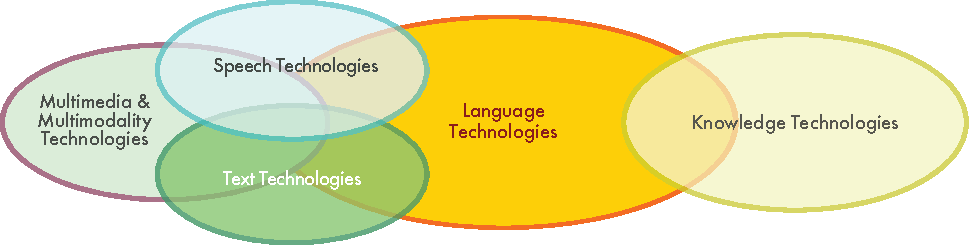
\includegraphics[width=\textwidth]{../_media/english/language_technologies}
  \caption{Language technology in context}
  \label{fig:ltincontext_en}
  \colorrule{grey3}{\textwidth}{1.5pt}
\end{figure*}

When we communicate, we combine language with other modes of communication and information media – for example speaking can involve gestures and facial expressions. Digital texts link to pictures and sounds. Movies may contain language in spoken and written form. In other words, speech and text technologies overlap and interact with other multimodal communication and multimedia technologies.\\ 
In this section, we will discuss the main application areas of language technology, i.\,e., language checking, web search, speech interaction, and machine translation. These applications and basic technologies include:

\begin{itemize}
\item spelling correction
\item authoring support
\item computer-assisted language learning
\item information retrieval 
\item information extraction
\item text summarisation
\item question answering
\item speech recognition 
\item speech synthesis 
\end{itemize}

Language technology is an established area of research with an extensive set of introductory literature.Those interested in finding out more about it should see the following references:  \cite{carstensen-etal1, jurafsky-martin01, manning-schuetze1, lt-world1, lt-survey1}.

Before discussing the above application areas, we will briefly describe the architecture of a typical LT system.

\subsection{Application Architectures}

Software applications for language processing typically consist of several components that mirror different aspects of language. While such applications are typically very complex, figure~\ref{fig:textprocessingarch_en} shows a highly simplified architecture of a typical text processing system. The first three modules handle the structure and meaning of the text input:

\begin{enumerate}
\item Pre-processing: cleans the data, analyses or removes formatting, detects the input languages, and so on.
\item Grammatical analysis: finds the verb, its objects, modifiers and other parts of speech; detects the sentence structure.
\item Semantic analysis: performs disambiguation (i.\,e., computes the appropriate meaning of words in a given context); resolves anaphora (i.\,e., which pronouns refer to which nouns in the sentence); represents the meaning of the sentence in a machine-readable way.
\end{enumerate}

After analysing the text, task-specific modules can perform other operations, such as automatic summarisation and database look-ups.

In the remainder of this section, we will firstly introduce the core application areas for language technology, and will follow this with a brief overview of the state of LT research and education today, and a description of past and present research programmes. Finally, we present an expert estimate of core LT tools and resources for Lithuanian in terms of various dimensions such as availability, maturity and quality. The general situation of LT for the Lithuanian language is summarised in a matrix (figure~\ref{fig:lrlttable_en}). Tools and resources that are boldfaced in the text can also be found in figure~\ref{fig:lrlttable_en} (p.~\pageref{fig:lrlttable_en}) at the end of this chapter. LT support for Lithuanian is also compared to other languages that are part of this series.

\begin{figure*}[htb]
  \colorrule{grey3}{\textwidth}{1.5pt}
  \center
  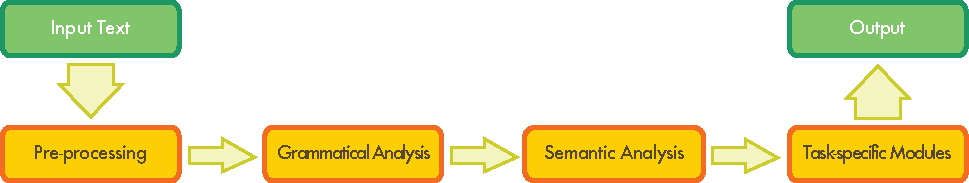
\includegraphics[width=\textwidth]{../_media/english/text_processing_app_architecture}
  \caption{A typical text processing architecture}
  \label{fig:textprocessingarch_en}
  \colorrule{grey3}{\textwidth}{1.5pt}
\end{figure*}

\subsection{Core Application Areas}

In this section, we focus on the most important LT tools and resources, and provide an overview of LT activities in Lithuania. 

\subsubsection{Language Checking}

Anyone who has used a word processor such as Microsoft Word knows that it has a spell checker that highlights spelling errors and proposes corrections. The first spelling correction programs compared a list of extracted words against a dictionary of correctly spelled words. Today these programs are far more sophisticated. Using language-dependent algorithms for \textbf{grammatical analysis}, they detect errors related to morphology (e.\,g., plural formation) as well as syntax–related errors, such as a missing verb or a conflict of verb-subject agreement (e.\,g., \textit{she *write a letter}). However, most spell checkers will not find any errors in the following text \cite{zar1}:

\begin{quote}
  I have a spelling checker,\\
  It came with my PC.\\
  It plane lee marks four my revue\\
  Miss steaks aye can knot sea.
\end{quote}


This type of analysis either needs to draw on language-specific \textbf{grammars} laboriously coded into the software by experts, or on a statistical language model. In this case, a model calculates the probability of a particular word as it occurs in a specific position (e.\,g., between the words that precede and follow it). For example: \textit{englische Buch} is a much more probable word sequence than \textit{Englisch Buch}. A statistical language model can be automatically created by using a large amount of (correct) language data, a \textbf{text corpus}. Most of these two approaches have been developed around data from English. Neither approach can transfer easily to Lithuanian because the language has a flexible word order and a richer inflection system (ever since 2002, scientists at Vytautas Magnus University have worked consistently with the statistical model of the Lithuanian language, which has its tools available for download \cite{airenas}).

\begin{figure*}[htb]
  \colorrule{grey3}{\textwidth}{1.5pt}
  \center
  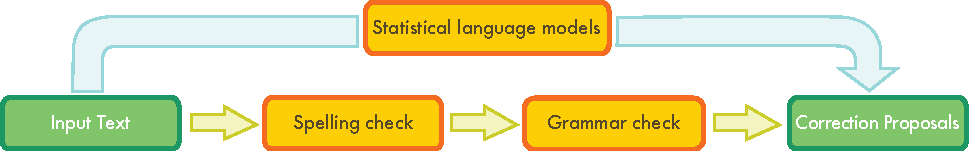
\includegraphics[width=\textwidth]{../_media/english/language_checking}
  \caption{Language checking (statistical; rule-based)}
  \label{fig:langcheckingaarch_en}
  \colorrule{grey3}{\textwidth}{1.5pt}
\end{figure*}

Language checking is not limited to word processors; it is also used in “authoring support systems”, i.\,e., software environments in which manuals and other types of technical documentation for complex IT, healthcare, engineering and other products, are written. To offset customer complaints about incorrect use and damage claims resulting from poorly understood instructions, companies are increasingly focusing on the quality of technical documentation while targeting the international market (via translation or localisation) at the same time. Advances in natural language processing have led to the development of authoring support software, which helps the writer of technical documentation to use vocabulary and sentence structures that are consistent with industry rules and (corporate) terminology restrictions.

\boxtext{The use of language checking is not limited to word processors. It also applies to authoring support systems.}

Only a few Lithuanian companies offer products in this area. In 1992-1994, Fotonija, UAB developed a spellchecking program \textit{Juodos Avys}, which has been subjected to ongoing upgrades. Automated spellchecking is based on an algorithm that helps avoiding spontaneous correction of a name or title for something else. Erroneous words are recognised and their correct versions are prompted. The program also prompts to correct missing specific Lithuanian characters like \textit{š}, \textit{ž},  \textit{ū}, \textit{ė}. The spellchecker has an integrated hyphenation tool for Lithuanian syllables.

In 2001 the spelling checker for Lithuanian was developed by Tilde IT, UAB. Tilde IT improves spelling checker and creates a new grammar checker that will analyse the sentence structure, identify missing and unnecessary commas or other punctuation marks, and check the syntax and lexical errors. The grammar checker will operate not only in Microsoft Office, but also in Open Office and on the Internet. It will be easily installable in other programs that use language items (e. g. enterprise resource management system, e. business solutions, etc.). Users will be able to try out the new grammar checker in 2012.

Besides spell checkers and authoring support, language checking is also important in the field of computer-assisted language learning. Language checking applications also automatically correct search engine queries, as found in Google's \textit{Did you mean…} prompts.

\subsubsection{Web Search}

\begin{figure*}[htb]
  \colorrule{grey3}{\textwidth}{1.5pt}
  \center
  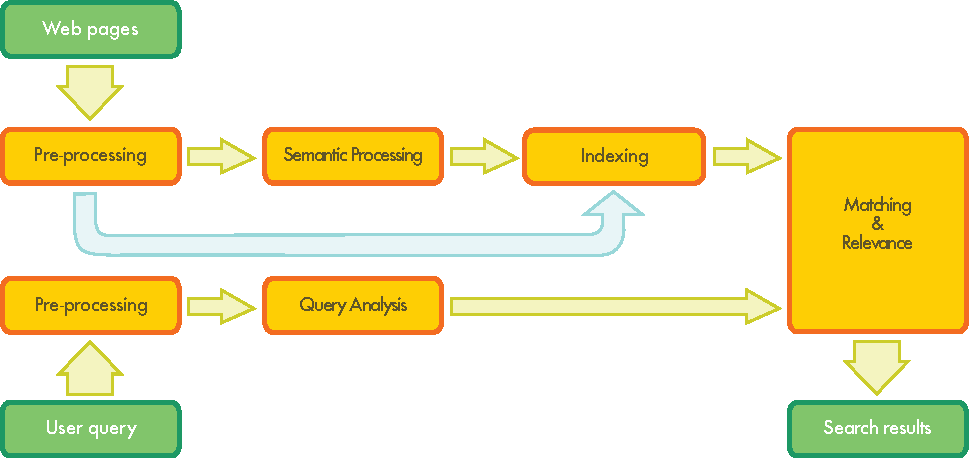
\includegraphics[width=\textwidth]{../_media/english/web_search_architecture}
  \caption{Web search}
  \label{fig:websearcharch_en}
  \colorrule{grey3}{\textwidth}{1.5pt}
 \end{figure*}

Searching the Web, intranets or digital libraries is probably the most widely used yet largely underdeveloped language technology application today. The Google search engine, which was launched in 1998, now handles about 80\% of all search queries \cite{spi1}. Since 2004, the verb \textit{googeln} has even had an entry in the Duden dictionary. The Google search interface and results page display has not significantly changed since the first version. However, in the current version, Google offers spelling correction for misspelled words and incorporates basic semantic search capabilities that can improve search accuracy by analysing the meaning of terms in a search query context \cite{pc1}. The Google success story shows that a large volume of data and efficient indexing techniques can deliver satisfactory results using a statistical approach to language processing. 

For more sophisticated information requests, it is essential to integrate deeper linguistic knowledge to facilitate text interpretation. Experiments using \textbf{lexical resources} such as machine-readable thesauri or ontological language resources (e.\,g., WordNet for English or GermaNet for German) have demonstrated improvements in finding pages using synonyms of the original search terms, such as \textit{Atomkraft} {[}atomic energy{]}, \textit{Kernenergie} {[}atomic power{]} and \textit{Nuklearenergie} {[}nuclear energy{]}, or even more loosely related terms.

\boxtext{The next generation of integrate search engines will have to include much more sophisticated language technology.}

The next generation of search engines will have to integrate much more sophisticated language technology, escpecially to deal with search queries consisting of a question or other sentence type rather than a list of keywords. For the query, \textit{Give me a list of all companies that were taken over by other companies in the last five years}, a syntactic as well as \textbf{semantic analysis} is required. The system also needs to provide an index to quickly retrieve relevant documents. A satisfactory answer will require syntactic parsing to analyse the grammatical structure of the sentence and determine that the user wants companies that have been acquired, rather than companies that have acquired other companies. For the expression \textit{last five years}, the system needs to determine the relevant range of years, taking into account the present year. The query then needs to be matched against a huge amount of unstructured data to find the pieces of information that are relevant to the user’s request. This process is called information retrieval, and involves searching and ranking relevant documents. To generate a list of companies, the system also needs to recognise a particular string of words in a document represents a company name, using a process called named entity recognition.

A more demanding challenge is matching a query in one language with documents in another language. Cross-lingual information retrieval involves automatically translating the query into all possible source languages and then translating the results back into the user's target language.

Now that data can be found in non-textual formats, increasingly often there is a need for services that deliver multimedia information retrieval by searching images, audio files and video data. In the case of audio and video files, a speech recognition module must convert the speech content into text (or into a phonetic representation) that can then be matched against a user query.

   In terms of the Lithuanian language, such technology is only in its early stage of development. Research and projects related to this area are conducted by Vytautas Magnus University (project \textit{Semantic Engine for Information Management} is supported by EU Structural Funds within the programme of economic growth activities), the Institute of Mathematics and Informatics of the University of Vilnius, Kaunas University of Technology. Several IT companies, such as Sintagma, UAB that has designed the document handling system \textit{Avilys} are taking their first steps in the field of designing ontologies, knowledge and document handling. Tilde IT, UAB has been developing semantic system projects since 2008 and is currently involved in the linguistic semantic network project SemTi as well as the international project SOLIM (\textit{Spatial Ontology Language for Multimedia Information Modeling}). Implementation of ontologies for some areas, like in library science is only now gaining speed.

    So far, any efforts in this area have been fragmented and any greater breakthrough is expected from the 2009-2013 programme of the Lithuanian language in information society as initiated by the government of the Republic of Lithuania, which programme envisages the development of tools designed to accommodate the providing of the syntactic/semantic analysis service, analysing Lithuanian website content, using it as a filter in searches, etc.

\subsubsection{Speech Interaction}

Speech interaction is one of many application areas that depend on speech technology, i.\,e., technologies for processing spoken language. Speech interaction technology is used to create interfaces that enable users to interact in spoken language instead of using a graphical display, keyboard and mouse.  Today, these voice user interfaces (VUI) are used for partially or fully automated telephone services provided by companies to customers, employees or partners. Business domains that rely heavily on VUIs include banking, supply chain, public transportation, and telecommunications. Other uses of speech interaction technology include interfaces with car navigation systems and the use of spoken language as an alternative to the graphical or touchscreen interfaces in smartphones.

\begin{figure*}[htb]
  \colorrule{grey3}{\textwidth}{1.5pt}
  \center
  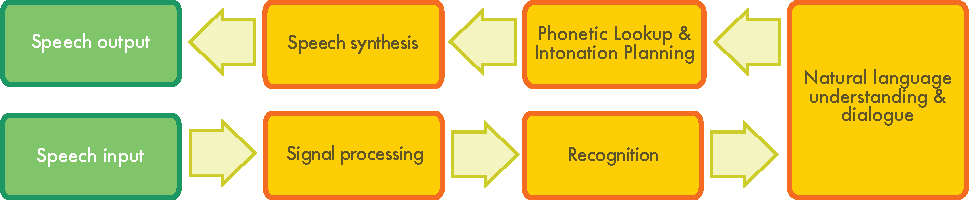
\includegraphics[width=\textwidth]{../_media/english/simple_speech-based_dialogue_architecture}
  \caption{Speech-based dialogue system}
  \label{fig:dialoguearch_en}
  \colorrule{grey3}{\textwidth}{1.5pt}
\end{figure*}

Speech interaction technology comprises four technologies: 

\begin{enumerate}
\item Automatic \textbf{speech recognition} (ASR) determines which words are actually spoken in a given sequence of sounds uttered by a user.  
\item Natural language understanding analyses the syntactic structure of a user’s utterance and interprets it according to the system in question.
\item Dialogue management determines which action to take given the user input and system functionality.   
\item \textbf{Speech synthesis} (text-to-speech or TTS) transforms the system’s reply into sounds for the user.
\end{enumerate}

One of the major challenges for ASR systems is to accurately recognise the words a user utters. This means restricting the range of possible user utterances to a limited set of keywords, or manually creating language models that cover a large range of natural language utterances. Using machine learning techniques, language models can also be generated automatically from \textbf{speech corpora}, i.\,e., large collections of speech audio files and text transcriptions. Restricting utterances usually forces people to use the voice user interface in a rigid way and can damage user acceptance; but the creation, tuning and maintenance of rich language models will significantly increase costs. VUIs that employ language models and initially allow a user to express their intent more flexibly — prompted by a \textit{How may I help you?} greeting — tend to be automated and are better received by users.

\boxtext{Speech interaction is the basis for creating interfaces that allow the user to interact with spoken language instead of a graphical dis-play, keyboard and mouse.}

Companies tend to use pre-recorded utterances by professional speakers for generating the output of the voice user interface. For static utterances where the wording does not depend on particular contexts of use or personal user data, this can deliver a rich user experience. But more dynamic content in an utterance may suffer from unnatural intonation because bits of audio files have simply been strung together. Through optimisation, today’s TTS systems are getting better at producing natural-sounding dynamic utterances.

Interfaces in speech interaction have been considerably standardised during the last decade in terms of their various technological components. There has also been strong market consolidation in speech recognition and speech synthesis. The national markets in the G20 countries (economically resilient countries with high populations) have been dominated by just five global players, with Nuance (USA) and Loquendo (Italy) being the most prominent players in Europe. In 2011, Nuance announced the acquisition of Loquendo, which represents a further step in market consolidation.

 Research into voice technology in Lithuania has been carried out at Kaunas University of Technology since 1980, with the Institute of Mathematics and Informatics of the University of Vilnius working in this field for many years as well; research in this area has been launched at Vytautas Magnus University too.

   In the Speech Research Laboratory (Kaunas University of Technology), ASR research was first started in 1980. The Laboratory has developed a corpus of commands and digital sequences. Lithuanian computer dialogs are being developed and a Lithuanian speech corpus, LTDIGITS, has been compiled and is now undergoing improvements. It contains continuous digit sequences and Lithuanian computer control words. Characteristics of Lithuanian speech are being researched at the Institute of Mathematics and Informatics of the University of Vilnius, which has compiled a corpus of broadcast news called LRNO. A universal corpus of spoken Lithuanian has been compiled by Vytautas Magnus University, which also compiles corpora of a smaller extent, like those designed to study the language, such as SACODEYL, a corpus of  spoken teenager language, etc., and research automated segmentation of spo-ken Lithuanian; development of automated transcription of spoken Lithuanian language is underway as well.

    Even though speech recognition research continues with the aim of improving the quality of this service, ASR software already has found successful application in law enforcement, telephony, education, transport, the Internet, etc.

Investigations in the text-to-speech synthesis and its application for the blind and partially sighted were carried out at Vilnius University. The most important components of the Lithuanian text-to-speech synthesiser \textit{Aistis} are: a) the automatic division of Lithuanian words into syllables; b) the automatic stressing of words in a Lithuanian text; c) the automatic transcription of Lithuanian text; d) a phonetic units base; e) Lithuanian text-to-speech synthesis quality evaluation. It is easy accessible and developed with a focus on applications for user groups with specific demands, such as physically handicapped people and the elderly. The synthesiser MBROLA is easily accessible on the Internet and runs on a base of phonetic units developed at the Vilnius University by Aleksas Girdenis and Pijus Kasparaitis.

The components of \textit{Aistis} were used in the development of the Lithuanian language synthesiser WinTalker Voice with two voices,  \textit{Gintaras} and  \textit{Aistis2}, which was produced by the Czech company Rosasoft on order from the Lithuanian Association of the Blind and Partially Sighted (there are a total of some 7,000 people with special needs in Lithuania and as of March 1, 2010 there were 258 blind persons using computers across Lithuania). Another free TTS synthesiser has been developed by  Etalinkas, UAB. The synthesiser runs under Windows and Linux OS.

For the purposes of speech recognition, Vytautas Magnus University has developed corpus-based statistical models of the Lithuanian language, a prototype of a continuous speech recognition tool that encompasses more than 1 million word forms, an automated accentuation programme with unambiguous homographs, which is available on the Internet, and models of durations of the Lithuanian language sounds.

Looking ahead, there will be significant changes, due to the spread of smartphones as a new platform for managing customer relationships, in addition to fixed telephones, the Internet and e-mail. This will also affect how speech interaction technology is used. In the long term, there will be fewer telephone-based VUIs, and spoken language apps will play a far more central role as a user-friendly input for smartphones. This will be largely driven by stepwise improvements in the accuracy of speaker-independent speech recognition via the speech dictation services already offered as centralised services to smartphone users.

\subsubsection{Machine Translation}

\begin{figure*}[htb]
  \colorrule{grey3}{\textwidth}{1.5pt}
  \center
  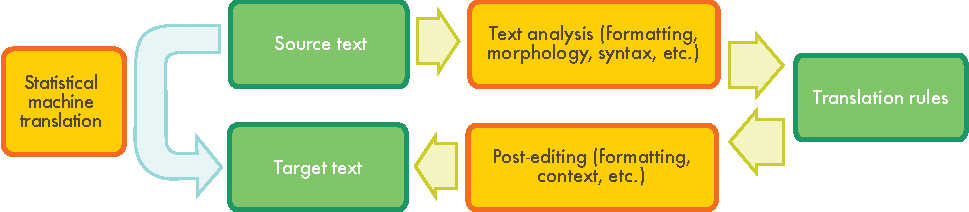
\includegraphics[width=\textwidth]{../_media/english/machine_translation}
  \caption{Machine translation (statistical; rule-based)}
  \label{fig:mtarch_en}
  \colorrule{grey3}{\textwidth}{1.5pt}
\end{figure*}

The idea of using digital computers to translate natural languages can be traced back to 1946 and was followed by substantial funding for research during the 1950s and again in the 1980s. 
Yet machine translation (MT) still cannot deliver on its initial promise of providing across-the-board automated translation.  

\boxtext{At its basic level, Machine Translation simply substitutes words in one natural language with words in another language.}

The most basic approach to machine translation is the automatic replacement of the words in a text written in one natural language with the equivalent words of another language. This can be useful in subject domains that have a very restricted, formulaic language such as weather reports.
However, in order to produce a good translation of less restricted texts, larger text units (phrases, sentences, or even whole passages) need to be matched to their closest counterparts in the target language. The major difficulty is that human language is ambiguous. Ambiguity creates challenges on multiple levels, such as word sense disambiguation on the lexical level (a \textit{jaguar} is a brand of car or an animal) or the assignment of case on the syntactic level, for example:\\
 \textit{I was happy to read a book.\\
      {[}Aš buvau laimingas:\\
      (a) perskaitęs knygą.\\
      (b) skaitydamas knygą.\\
      (c) galėdamas perskaityti knygą.] }

One way to build an MT system is to use linguistic rules. For translations between closely related languages, a translation using direct substitution may be feasible in cases such as the above example. However, rule-based (or linguistic knowledge-driven) systems often analyse the input text and create an intermediary symbolic representation from which the target language text can be generated. The success of these methods is highly dependent on the availability of extensive lexicons with morphological, syntactic, and semantic information, and large sets of grammar rules carefully designed by skilled linguists. This is a very long and therefore costly process.

In the late 1980s, when computational power increased and became cheaper, interest in statistical models for machine translation began to grow. Statistical models are derived from analysing bilingual text corpora, \textbf{parallel corpora}, such as the Europarl parallel corpus, which contains the proceedings of the European Parliament in 11 European languages. Given enough data, statistical MT works well enough to derive an approximate meaning of a foreign language text by processing parallel versions and finding plausible patterns of words. Unlike knowledge-driven systems, however, statistical (or data-driven) MT systems often generate ungrammatical output. Data-driven MT is advantageous because less human effort is required, and it can also cover special particularities of the language (e.\,g., idiomatic expressions) that are often ignored in knowledge-driven systems. 

The strengths and weaknesses of knowledge-driven and data-driven machine translation tend to be complementary, so that nowadays researchers focus on hybrid approaches that combine both methodologies. One such approach uses both knowledge-driven and data-driven systems, together with a selection module that decides on the best output for each sentence. However, results for sentences longer than, say, 12 words, will often be far from perfect. A more effective solution is to combine the best parts of each sentence from multiple outputs; this can be fairly complex, as corresponding parts of multiple alternatives are not always obvious and need to be aligned. 

\boxtext{Machine Translation is particularly challenging for the Lithuanian language.}

Machine translation is particularly challenging for the Lithuanian language. Free word order and verb constructions pose problems for analysis, and inflection is a challenge for generating words with proper gender and case markings. 

    With languages that have a smaller user base, such as the Baltic languages MT research tools, as well as language technologies in general, are less developed. There have been several activities related to MT in Lithuania. There are three translation tools currently available on the web: WIFTA project \cite{vertvdu},  Google translator and \textit{Vertimo Vedlys} \cite{mvlab}.  The first system was developed in 2008 in cooperation with the Russian company ProMT and is based on rule-based technology. It performs MT that takes into account the morphological, syntactic and semantic properties of texts. This project was finished successfully. The English-Lithuanian MT system has been in operation at http://vertimas.vdu.lt since 2008. It generates 127 million hits and attracts approximately 1 million unique users yearly. Registered users have access to computer and business thesauruses.

    The corpus of the written Lithuanian language, which has been compiled at Vytautas Magnus University and contains ap. 140 million words, is open to the public over the Internet \cite{tekstynas}.  Further-more, a parallel corpus of the Lithuanian language and other lan-guages (English, German, Czech) is being compiled, other special corpora have been developed as well (for instance, the University of Vilnius has compiled a Corpus of Academic Lithuanian \textit{CorALit} \cite{coralit}). However, the current corpus of the Lithuanian language cannot accommodate the needs of the development of modern technologies (like search for information, automated translation and other systems) of the Lithuanian language. The existing and future corpora require software customised to the Lithuanian language that would allow making better use of the available language resources and the digital descriptions that they produce. One of the prerequisites for classical SMT systems is the  availability of a large parallel corpus which computer then uses in the training process. The lack of a large parallel corpus is the main reason why experiments with SMT in the Baltic countries have only started recently.  

The Google MT software uses the SMT approach and provides MT for about 30 languages, including the Lithuanian language.

\textit{Vertimo Vedlys } is a machine translation experimental tool developed by the Institute of the Lithuanian Language in association with Tilde IT, UAB. The trial version provides translation from Lithuanian to English. The automated translation tool analyses the structure of sentences and automatically prompts a translation of a sentence, its part or individual words. It is based on SMT and uses Giza ++ and Moses engines. Tilde IT is developing a Lithuanian-English machine translation system by integrating statistical and rule-based MT methods as well as by applying an innovative processing of multiword expressions. The accuracy of translation is 30\%. The system is constantly improved. "Tilde's IT“ MT has been used not only for full text translation but also in cross-lingual search applications.

There is still a huge potential for improving the quality of MT systems. The challenges involve adapting language resources to a given subject domain or user area, and integrating the technology into workflows that already have term bases and translation memories. Another problem is that most of the current systems are English-centred and only support a few languages that can be translated to Lithuanian and vice -- versa. This leads to friction in the translation workflow and forces MT users to learn different lexicon coding tools for different systems.

Evaluation campaigns help to compare the quality of MT systems, the different approaches and the status of the systems for different language pairs. Figure~\ref{fig:euromatrix_de} (p.~\pageref{fig:euromatrix_de}), which was prepared during the EC Euromatrix+ project, shows the pair-wise performances obtained for 22 of the 23 official EU languages (Irish was not compared). The results are ranked according to a BLEU score, which indicates higher scores for better translations \cite{bleu1}. A human translator would normally achieve a score of around 80 points.

The best results highlighted (in green and blue) were achieved by languages that benefit from a considerable research effort in coordinated programmes and the existence of many parallel corpora (e.\,g., English, French, Dutch, Spanish and German). The languages with poorer results are shown in red. These languages either lack such development efforts or are structurally very different from other languages (e.\,g., Hungarian, Maltese and Finnish).

\begin{figure*}[htbp]
  \centering
  \setlength{\tabcolsep}{0.17em}
  \small
  \begin{tabular}{>{\columncolor{corange1}}cccccccccccccccccccccccc}
    & \multicolumn{22}{>{\columncolor{corange1}}c}{Zielsprache -- \textcolor{grey1}{Target language}}\\\addlinespace[{-.009cm}]
    \rowcolor{corange1}  & EN & BG & DE & CS & DA & EL & ES & ET & FI & FR & HU & IT & LT & LV & MT & NL & PL & PT & RO & SK & SL & SV\\
    EN & -- & \textcolor{blue}{40.5} & \textcolor{blue}{46.8} & \textcolor{green2}{52.6} & \textcolor{green2}{50.0} & \textcolor{blue}{41.0} & \textcolor{green2}{55.2} & \textcolor{purple}{34.8} & \textcolor{purple}{38.6} & \textcolor{green2}{50.1} & \textcolor{purple}{37.2} & \textcolor{green2}{50.4} & \textcolor{purple}{39.6} & \textcolor{blue}{43.4} & \textcolor{purple}{39.8} & \textcolor{green2}{52.3} & \textcolor{blue}{49.2} & \textcolor{green2}{55.0} & \textcolor{blue}{49.0} & \textcolor{blue}{44.7} & \textcolor{green2}{50.7} & \textcolor{green2}{52.0}\\
    BG & \textcolor{green}{61.3} & -- & \textcolor{purple}{38.7} & \textcolor{purple}{39.4} & \textcolor{purple}{39.6} & \textcolor{purple}{34.5} & \textcolor{blue}{46.9} & \textcolor{red3}{25.5} & \textcolor{red3}{26.7} & \textcolor{blue}{42.4} & \textcolor{red3}{22.0} & \textcolor{blue}{43.5} & \textcolor{red3}{29.3} & \textcolor{red3}{29.1} & \textcolor{red3}{25.9} & \textcolor{blue}{44.9} & \textcolor{purple}{35.1} & \textcolor{blue}{45.9} & \textcolor{purple}{36.8} & \textcolor{purple}{34.1} & \textcolor{purple}{34.1} & \textcolor{purple}{39.9}\\
    DE & \textcolor{green2}{53.6} & \textcolor{red3}{26.3} & -- & \textcolor{purple}{35.4} & \textcolor{blue}{43.1} & \textcolor{purple}{32.8} & \textcolor{blue}{47.1} & \textcolor{red3}{26.7} & \textcolor{red3}{29.5} & \textcolor{purple}{39.4} & \textcolor{red3}{27.6} & \textcolor{blue}{42.7} & \textcolor{red3}{27.6} & \textcolor{purple}{30.3} & \textcolor{red2}{19.8} & \textcolor{green2}{50.2} & \textcolor{purple}{30.2} & \textcolor{blue}{44.1} & \textcolor{purple}{30.7} & \textcolor{red3}{29.4} & \textcolor{purple}{31.4} & \textcolor{blue}{41.2}\\
    CS & \textcolor{green2}{58.4} & \textcolor{purple}{32.0} & \textcolor{blue}{42.6} & -- & \textcolor{blue}{43.6} & \textcolor{purple}{34.6} & \textcolor{blue}{48.9} & \textcolor{purple}{30.7} & \textcolor{purple}{30.5} & \textcolor{blue}{41.6} & \textcolor{red3}{27.4} & \textcolor{blue}{44.3} & \textcolor{purple}{34.5} & \textcolor{purple}{35.8} & \textcolor{red3}{26.3} & \textcolor{blue}{46.5} & \textcolor{purple}{39.2} & \textcolor{blue}{45.7} & \textcolor{purple}{36.5} & \textcolor{blue}{43.6} & \textcolor{blue}{41.3} & \textcolor{blue}{42.9}\\
    DA & \textcolor{green2}{57.6} & \textcolor{red3}{28.7} & \textcolor{blue}{44.1} & \textcolor{purple}{35.7} & -- & \textcolor{purple}{34.3} & \textcolor{blue}{47.5} & \textcolor{red3}{27.8} & \textcolor{purple}{31.6} & \textcolor{blue}{41.3} & \textcolor{red3}{24.2} & \textcolor{blue}{43.8} & \textcolor{red3}{29.7} & \textcolor{purple}{32.9} & \textcolor{red3}{21.1} & \textcolor{blue}{48.5} & \textcolor{purple}{34.3} & \textcolor{blue}{45.4} & \textcolor{purple}{33.9} & \textcolor{purple}{33.0} & \textcolor{purple}{36.2} & \textcolor{blue}{47.2}\\
    EL & \textcolor{green2}{59.5} & \textcolor{purple}{32.4} & \textcolor{blue}{43.1} & \textcolor{purple}{37.7} & \textcolor{blue}{44.5} & -- & \textcolor{green2}{54.0} & \textcolor{red3}{26.5} & \textcolor{red3}{29.0} & \textcolor{blue}{48.3} & \textcolor{red3}{23.7} & \textcolor{blue}{49.6} & \textcolor{red3}{29.0} & \textcolor{purple}{32.6} & \textcolor{red3}{23.8} & \textcolor{blue}{48.9} & \textcolor{purple}{34.2} & \textcolor{green2}{52.5} & \textcolor{purple}{37.2} & \textcolor{purple}{33.1} & \textcolor{purple}{36.3} & \textcolor{blue}{43.3}\\
    ES & \textcolor{green}{60.0} & \textcolor{purple}{31.1} & \textcolor{blue}{42.7} & \textcolor{purple}{37.5} & \textcolor{blue}{44.4} & \textcolor{purple}{39.4} & -- & \textcolor{red3}{25.4} & \textcolor{red3}{28.5} & \textcolor{green2}{51.3} & \textcolor{red3}{24.0} & \textcolor{green2}{51.7} & \textcolor{red3}{26.8} & \textcolor{purple}{30.5} & \textcolor{red3}{24.6} & \textcolor{blue}{48.8} & \textcolor{purple}{33.9} & \textcolor{green2}{57.3} & \textcolor{purple}{38.1} & \textcolor{purple}{31.7} & \textcolor{purple}{33.9} & \textcolor{blue}{43.7}\\
    ET & \textcolor{green2}{52.0} & \textcolor{red3}{24.6} & \textcolor{purple}{37.3} & \textcolor{purple}{35.2} & \textcolor{purple}{37.8} & \textcolor{red3}{28.2} & \textcolor{blue}{40.4} & -- & \textcolor{purple}{37.7} & \textcolor{purple}{33.4} & \textcolor{purple}{30.9} & \textcolor{purple}{37.0} & \textcolor{purple}{35.0} & \textcolor{purple}{36.9} & \textcolor{red3}{20.5} & \textcolor{blue}{41.3} & \textcolor{purple}{32.0} & \textcolor{purple}{37.8} & \textcolor{red3}{28.0} & \textcolor{purple}{30.6} & \textcolor{purple}{32.9} & \textcolor{purple}{37.3}\\
    FI & \textcolor{blue}{49.3} & \textcolor{red3}{23.2} & \textcolor{purple}{36.0} & \textcolor{purple}{32.0} & \textcolor{purple}{37.9} & \textcolor{red3}{27.2} & \textcolor{purple}{39.7} & \textcolor{purple}{34.9} & -- & \textcolor{red3}{29.5} & \textcolor{red3}{27.2} & \textcolor{purple}{36.6} & \textcolor{purple}{30.5} & \textcolor{purple}{32.5} & \textcolor{red2}{19.4} & \textcolor{blue}{40.6} & \textcolor{red3}{28.8} & \textcolor{purple}{37.5} & \textcolor{red3}{26.5} & \textcolor{red3}{27.3} & \textcolor{red3}{28.2} & \textcolor{purple}{37.6}\\
    FR & \textcolor{green}{64.0} & \textcolor{purple}{34.5} & \textcolor{blue}{45.1} & \textcolor{purple}{39.5} & \textcolor{blue}{47.4} & \textcolor{blue}{42.8} & \textcolor{green}{60.9} & \textcolor{red3}{26.7} & \textcolor{purple}{30.0} & -- & \textcolor{red3}{25.5} & \textcolor{green2}{56.1} & \textcolor{red3}{28.3} & \textcolor{purple}{31.9} & \textcolor{red3}{25.3} & \textcolor{green2}{51.6} & \textcolor{purple}{35.7} & \textcolor{green}{61.0} & \textcolor{blue}{43.8} & \textcolor{purple}{33.1} & \textcolor{purple}{35.6} & \textcolor{blue}{45.8}\\
    HU & \textcolor{blue}{48.0} & \textcolor{red3}{24.7} & \textcolor{purple}{34.3} & \textcolor{purple}{30.0} & \textcolor{purple}{33.0} & \textcolor{red3}{25.5} & \textcolor{purple}{34.1} & \textcolor{red3}{29.6} & \textcolor{red3}{29.4} & \textcolor{purple}{30.7} & -- & \textcolor{purple}{33.5} & \textcolor{red3}{29.6} & \textcolor{purple}{31.9} & \textcolor{red2}{18.1} & \textcolor{purple}{36.1} & \textcolor{red3}{29.8} & \textcolor{purple}{34.2} & \textcolor{red3}{25.7} & \textcolor{red3}{25.6} & \textcolor{red3}{28.2} & \textcolor{purple}{30.5}\\
    IT & \textcolor{green}{61.0} & \textcolor{purple}{32.1} & \textcolor{blue}{44.3} & \textcolor{purple}{38.9} & \textcolor{blue}{45.8} & \textcolor{blue}{40.6} & \textcolor{red3}{26.9} & \textcolor{red3}{25.0} & \textcolor{red3}{29.7} & \textcolor{green2}{52.7} & \textcolor{red3}{24.2} & -- & \textcolor{red3}{29.4} & \textcolor{purple}{32.6} & \textcolor{red3}{24.6} & \textcolor{green2}{50.5} & \textcolor{purple}{35.2} & \textcolor{green2}{56.5} & \textcolor{purple}{39.3} & \textcolor{purple}{32.5} & \textcolor{purple}{34.7} & \textcolor{blue}{44.3}\\
    LT & \textcolor{green2}{51.8} & \textcolor{red3}{27.6} & \textcolor{purple}{33.9} & \textcolor{purple}{37.0} & \textcolor{purple}{36.8} & \textcolor{red3}{26.5} & \textcolor{red3}{21.1} & \textcolor{purple}{34.2} & \textcolor{purple}{32.0} & \textcolor{purple}{34.4} & \textcolor{red3}{28.5} & \textcolor{purple}{36.8} & -- & \textcolor{blue}{40.1} & \textcolor{red3}{22.2} & \textcolor{purple}{38.1} & \textcolor{purple}{31.6} & \textcolor{purple}{31.6} & \textcolor{red3}{29.3} & \textcolor{purple}{31.8} & \textcolor{purple}{35.3} & \textcolor{purple}{35.3}\\
    LV & \textcolor{green2}{54.0} & \textcolor{red3}{29.1} & \textcolor{purple}{35.0} & \textcolor{purple}{37.8} & \textcolor{purple}{38.5} & \textcolor{red3}{29.7} & \textcolor{red2}{8.0} & \textcolor{purple}{34.2} & \textcolor{purple}{32.4} & \textcolor{purple}{35.6} & \textcolor{red3}{29.3} & \textcolor{purple}{38.9} & \textcolor{purple}{38.4} & -- & \textcolor{red3}{23.3} & \textcolor{blue}{41.5} & \textcolor{purple}{34.4} & \textcolor{purple}{39.6} & \textcolor{purple}{31.0} & \textcolor{purple}{33.3} & \textcolor{purple}{37.1} & \textcolor{purple}{38.0}\\
    MT & \textcolor{green}{72.1} & \textcolor{purple}{32.2} & \textcolor{purple}{37.2} & \textcolor{purple}{37.9} & \textcolor{purple}{38.9} & \textcolor{purple}{33.7} & \textcolor{blue}{48.7} & \textcolor{red3}{26.9} & \textcolor{red3}{25.8} & \textcolor{blue}{42.4} & \textcolor{red3}{22.4} & \textcolor{blue}{43.7} & \textcolor{purple}{30.2} & \textcolor{purple}{33.2} & -- & \textcolor{blue}{44.0} & \textcolor{purple}{37.1} & \textcolor{blue}{45.9} & \textcolor{purple}{38.9} & \textcolor{purple}{35.8} & \textcolor{blue}{40.0} & \textcolor{blue}{41.6}\\
    NL & \textcolor{green2}{56.9} & \textcolor{red3}{29.3} & \textcolor{blue}{46.9} & \textcolor{purple}{37.0} & \textcolor{blue}{45.4} & \textcolor{purple}{35.3} & \textcolor{blue}{49.7} & \textcolor{red3}{27.5} & \textcolor{red3}{29.8} & \textcolor{blue}{43.4} & \textcolor{red3}{25.3} & \textcolor{blue}{44.5} & \textcolor{red3}{28.6} & \textcolor{purple}{31.7} & \textcolor{red3}{22.0} & -- & \textcolor{purple}{32.0} & \textcolor{blue}{47.7} & \textcolor{purple}{33.0} & \textcolor{purple}{30.1} & \textcolor{purple}{34.6} & \textcolor{blue}{43.6}\\
    PL & \textcolor{green}{60.8} & \textcolor{purple}{31.5} & \textcolor{blue}{40.2} & \textcolor{blue}{44.2} & \textcolor{blue}{42.1} & \textcolor{purple}{34.2} & \textcolor{blue}{46.2} & \textcolor{red3}{29.2} & \textcolor{red3}{29.0} & \textcolor{blue}{40.0} & \textcolor{red3}{24.5} & \textcolor{blue}{43.2} & \textcolor{purple}{33.2} & \textcolor{purple}{35.6} & \textcolor{red3}{27.9} & \textcolor{blue}{44.8} & -- & \textcolor{blue}{44.1} & \textcolor{purple}{38.2} & \textcolor{purple}{38.2} & \textcolor{purple}{39.8} & \textcolor{blue}{42.1}\\
    PT & \textcolor{green}{60.7} & \textcolor{purple}{31.4} & \textcolor{blue}{42.9} & \textcolor{purple}{38.4} & \textcolor{blue}{42.8} & \textcolor{blue}{40.2} & \textcolor{green}{60.7} & \textcolor{red3}{26.4} & \textcolor{red3}{29.2} & \textcolor{green2}{53.2} & \textcolor{red3}{23.8} & \textcolor{green2}{52.8} & \textcolor{red3}{28.0} & \textcolor{purple}{31.5} & \textcolor{red3}{24.8} & \textcolor{blue}{49.3} & \textcolor{purple}{34.5} & -- & \textcolor{purple}{39.4} & \textcolor{purple}{32.1} & \textcolor{purple}{34.4} & \textcolor{blue}{43.9}\\
    RO & \textcolor{green}{60.8} & \textcolor{purple}{33.1} & \textcolor{purple}{38.5} & \textcolor{purple}{37.8} & \textcolor{blue}{40.3} & \textcolor{purple}{35.6} & \textcolor{green2}{50.4} & \textcolor{red3}{24.6} & \textcolor{red3}{26.2} & \textcolor{blue}{46.5} & \textcolor{red3}{25.0} & \textcolor{blue}{44.8} & \textcolor{red3}{28.4} & \textcolor{red3}{29.9} & \textcolor{red3}{28.7} & \textcolor{blue}{43.0} & \textcolor{purple}{35.8} & \textcolor{blue}{48.5} & -- & \textcolor{purple}{31.5} & \textcolor{purple}{35.1} & \textcolor{purple}{39.4}\\
    SK & \textcolor{green}{60.8} & \textcolor{purple}{32.6} & \textcolor{purple}{39.4} & \textcolor{blue}{48.1} & \textcolor{blue}{41.0} & \textcolor{purple}{33.3} & \textcolor{blue}{46.2} & \textcolor{red3}{29.8} & \textcolor{red3}{28.4} & \textcolor{purple}{39.4} & \textcolor{red3}{27.4} & \textcolor{blue}{41.8} & \textcolor{purple}{33.8} & \textcolor{purple}{36.7} & \textcolor{red3}{28.5} & \textcolor{blue}{44.4} & \textcolor{purple}{39.0} & \textcolor{blue}{43.3} & \textcolor{purple}{35.3} & -- & \textcolor{blue}{42.6} & \textcolor{blue}{41.8}\\
    SL & \textcolor{green}{61.0} & \textcolor{purple}{33.1} & \textcolor{purple}{37.9} & \textcolor{blue}{43.5} & \textcolor{blue}{42.6} & \textcolor{purple}{34.0} & \textcolor{blue}{47.0} & \textcolor{purple}{31.1} & \textcolor{red3}{28.8} & \textcolor{purple}{38.2} & \textcolor{red3}{25.7} & \textcolor{blue}{42.3} & \textcolor{purple}{34.6} & \textcolor{purple}{37.3} & \textcolor{purple}{30.0} & \textcolor{blue}{45.9} & \textcolor{purple}{38.2} & \textcolor{blue}{44.1} & \textcolor{purple}{35.8} & \textcolor{purple}{38.9} & -- & \textcolor{blue}{42.7}\\
    SV & \textcolor{green2}{58.5} & \textcolor{red3}{26.9} & \textcolor{blue}{41.0} & \textcolor{purple}{35.6} & \textcolor{blue}{46.6} & \textcolor{purple}{33.3} & \textcolor{blue}{46.6} & \textcolor{red3}{27.4} & \textcolor{purple}{30.9} & \textcolor{purple}{38.9} & \textcolor{red3}{22.7} & \textcolor{blue}{42.0} & \textcolor{red3}{28.2} & \textcolor{purple}{31.0} & \textcolor{red3}{23.7} & \textcolor{blue}{45.6} & \textcolor{purple}{32.2} & \textcolor{blue}{44.2} & \textcolor{purple}{32.7} & \textcolor{purple}{31.3} & \textcolor{purple}{33.5} & --\\
    \end{tabular}
  \caption{Machine translation between 22 EU-languages \cite{euro1}}
  \label{fig:euromatrix_de}
\end{figure*}


\subsection{Other Application Areas}

Building language technology applications involves a range of subtasks that do not always surface at the level of interaction with the user, but they provide significant service functionalities “behind the scenes” of the system in question. They all form important research issues that have now evolved into individual sub-disciplines of computational linguistics.  Question answering, for example, is an active area of research for which annotated corpora have been built and scientific competitions have been initiated. The concept of question answering goes beyond keyword-based searches (in which the search engine responds by delivering a collection of potentially relevant documents) and enables users to ask a concrete question to which the system provides a single answer. For example:

\textit{Question: How old was Neil Armstrong when he stepped on the moon?}\\
\textit{Answer: 38.}

While question answering is obviously related to the core area of web search, it is nowadays an umbrella term for such research issues as which different types of questions exist, and how they should be handled; how a set of documents that potentially contain the answer can be analysed and compared (do they provide conflicting answers?); and how specific information (the answer) can be reliably extracted from a document without ignoring the context. 

\boxtext{Language technology applications often provide significant service functionalities "behind the scenes” of larger software systems.}

Question answering is in turn related to information extraction (IE), an area that was extremely popular and influential when computational linguistics took a statistical turn in the early 1990s. IE aims to identify specific pieces of information in specific classes of documents, such as the key players in company takeovers as reported in newspaper stories. Another common scenario that has been studied is reports on terrorist incidents. The task here consists of mapping appropriate parts of the text to a template that specifies the perpetrator, target, time, location and results of the incident. Domain-specific template-filling is the central characteristic of IE, which makes it another example of a “behind the scenes” technology that forms a well-demarcated research area, which in practice needs to be embedded into a suitable application environment. 

    Text summarisation and \textbf{text generation} are two borderline areas that can act either as standalone applications or play a supporting role. Summarisation attempts to give the essentials of a long text in a short form, and is one of the features available in Microsoft Word. It mostly uses a statistical approach to identify the “important” words in a text (i.\,e., words that occur very frequently in the text in question but less frequently in general language use) and determine which sentences contain the most of these “important” words. These sentences are then extracted and put together to create a summary. In this very common commercial scenario, summarisation is simply a form of sentence extraction, and the text is reduced to a subset of its sentences. An alternative approach, for which some research has been carried out, is to generate brand new sentences that do not exist in the source text. 

This requires a deeper understanding of the text, which means that so far this approach is far less robust. On the whole, a text generator is rarely used as a stand-alone application but is embedded into a larger software environment, such as a clinical information system that collects, stores and processes patient data. Creating reports is just one of many applications for text summarisation. 

 For Lithuanian, the situation in all these research areas is much less developed than it is with the English language: some experiments have been performed on Lithuanian text summarization, automatic identification of educational and scientific terminology (in Vytautas Magnus University), etc.

Lithuanian has been included in the international projects that the Latvia-based CIA Tilde carries out. Prototypes of Lithuanian information retrieval engines were developed as part of FP5 project CLARITY: A proposal for cross-language information retrieval and organisation of text and audio documents. The CLARITY cross-language information retrieval system was developed for the following language pairs:  English-Latvian, Latvian-English, German-Latvian, Latvian-German, Russian-Latvian, Latvian-Russian, Lithuanian English, English-Lithuanian, German-Lithuanian, Lithuanian-German, Lithuanian-Russian and Russian German. With respect to the Baltic languages, the results for document retrieval using direct query translation indicate that the average precision can reach a level of more than 70\% compared to monolingual retrieval.

\subsection{Educational Programmes}

 Language technology is a very interdisciplinary field that involves the combined expertise of linguists, computer scientists, mathematicians, philosophers, psycholinguists, and neuroscientists among others. As a result, it has not acquired a clear, independent existence in the Lithuanian faculty system. Some universities have established separate centres for Computational Linguistics (CL), e.g. Vytautas Magnus University, or laboratories, e.g. the Speech Research Laboratory in Kaunas University of Technology. Currently, there is only one curriculum for bachelor studies of Computational Linguistics in the Faculty of Humanities in Kaunas University of Technologies. The program was launched in 2003, and had had 73 graduates by 2010. The steadily rising demand of qualified personnel specialised in the field of Language Technology cannot be met by the comparably low number of graduates.

    In Vilnius University and Vytautas Magnus University some CL- and LT-related courses are taught as part of other studies. As of 2011, the Kaunas Humanities Faculty of the University of Vilnius offers master courses of audiovisual translation. Vytautas Magnus University has had a master programme of digital linguistics  since 2006 (accredited until 2015). As yet, no university offers consistent studies of every level, and therefore the field of linguistic technologies employs scientists who have completed linguistic or informatics studies (some of them both). A scientific research base is being developed and resources compiled at the Institute of Mathematics and Informatics and the Institute of the Lithuanian Language; the latter establishment founded a Digital Language Resources Laboratory in 2010.

\subsection{National Projects and Initiatives}

A higher degree of expansion of the information society, a lively interest in language technologies, and the development of resources in Lithuania only started a few decades ago. Since the Lithuanian language has a rather limited number of users, the commercial market for language technologies is not very big and besides, Lithuania has no such modern technological giants as BMW or NOKIA, and there are merely a few commercial businesses operating on the LT field.  

Most of the initiative and commitment with regard to the functioning of the Lithuanian language within the information society and LT development originates on the national level. The year 2000 saw the launch of the first national programme of the Lithuanian language in the information society for the period of 2000–2006. The programme is coordinated by the State Commission of the Lithuanian Language and that deals with localisation, resource and tool creation, documentation and some other activities:
\begin{itemize}
      \item ASR expansion, involving research of the traits of the Lithuanian speech, development of a prototype recognition tool for separate spoken words, improvement of the spoken corpus of Lithuanian broadcast news LRNO, studies of Lithuanian computerised voice dialogs, improvement of the quality of TTS synthesis, development of pilot samples of application of Lithuanian voice technologies, automated segmentation of the Lithuanian spoken language and development of automated transcription of the Lithuanian speech.
      \item Standardisation of the Lithuanian language subjects in IT, involving the development of the computer font \textit{Palemonas}, localisation, etc.
      \item Translation and the development of the necessary resources and tools, involving the development of a computerised system for literal translation of specialised texts, development of a parallel corpus of the Lithuanian and the Czech languages, as later updated, development of a tool of morphological analysis and generation.
      \item Work has been started in the field of syntactic and semantic analysis of texts in the Lithuanian language. 
          \end{itemize}

    The Information Society Development Committee under the Ministry of Transport and Communications is responsible for the second phase of the program of the Lithuanian Language in the Information Society 2009-2013. The programme provides for the creation of an Internet portal with free access to all the available language resources and technologies, augmentation of the existing and newly created linguistic resources, improvement of the ASR and TTS technologies, new MT tools, improvement and development of semantic and syntactic analysis and search tools.

Research any resource generation in this area is promoted as well. The Lithuanian Research Council has launched the first national program "State and Nation: Heritage and Identity" that encompasses digitalization of intangible heritage (this program saw the implementation of the project called "Development of a Lituanistic Digital Resource Metadata System out its Compatibility with CLARIN"). Recently, The Lithuanian Council of Sciences also finances the programme for the Development of National Lituanistics 2009–2015, aimed at developing and promoting lituanistic research, helping meet the priority of lituanistic research, strengthening the input of lituanistic research data into the overall expansion of nation-wide humanistic, providing a scientific base for nurturing national self-consciousness and protecting lituanistic heritage.
Companies doing business on the field of language technology are few and include Tildė IT, UAB, Fotonija, UAB, Microsoft Lietuva, UAB, CID Baltic, Synergium, Sintagma, TokenMill, HLTech.
Tilde IT, UAB is the clear leader in the area of language technology, with 12 years of experience of operating on the Lithuanian market.
The company is giving a lot of attention to software localisation, translations of technical documentation, development of software to support the Lithuanian language. Tilde IT is one of the largest providers of localisation services in Lithuania. The company works together with international localisation and translation companies on a continuous basis.

    At this time, Tilde IT is engaged in improving the quality of machine translation and the development and upgrade of spellchecking systems. The company initiates research and technological development projects aimed at developing prototype software in cooperation with the Institute of the Lithuanian Language and the Institute of Mathematics of Informatics, as well as the Philological Faculty of the University of Vilnius.

    Tilde IT has been conducting semantic system projects since 2008. Since Tilde IT is involved in providing machine translation technologies for the European market, the new technology will be used as an addition to the set of techniques that improve machine translation results. Tilde IT aims to create a database of links between Lithuanian words, also known as a linguistic semantic database. A Lithuanian semantic web would greatly help marketing professionals because it would help to predict public reaction to the proposed product promotions, packaging or name. Therefore, such a thinking map can be used to create new products and the generation of new or original ideas. One word can have more than 15 synonyms, although ordinarily people only know just 5 to 6 of them. A detailed semantic web will help save the Lithuanian language’s synonymic diversity. 

   Tilde IT has joined SOLIM (Spatial Ontology Language for multimedia Information Modelling) project of the Eurostars program. The project is aimed to improve context aware information analysis to venture beyond a static world, by adding the concepts of space and change. The goal of the project is to extend the Web Ontology Language OWL to support effective storage and reasoning on spatial information, and to demonstrate the power of such extension for automatic processing of textual and graphical information in real proof of concept applications. 

    As of 1991, Fotonija, UAB has been integrating the Lithuanian language into the computer environment by developing and upgrading drivers (\textit{WinLika}, \textit{Lika}), designing a Lithuanian font dubbed \textit{Aistika}, the text management application \textit{Mainukai}, the document converter, the text creation, editing and proofing application, and the spellchecker \textit{Juodos Avys}. An important area of "Fotonija’s" business is the development of monolingual and multilingual dictionaries, which include the international word dictionary \textit{Interleksis}, TŽŽ, the English-Lithuanian dictionary \textit{Anglonas}, and its French counterpart, \textit{Frankonas}.  

There are other companies engaging in localisation, ontology development and other LT projects as well, including Microsoft Lietuva, CID Baltic, Synergium, Sintagma, TokenMill, HLTech,and so on. 

    As we have seen, previous programmes have led to the development of a number of LT tools and resources for the Lithuanian language. In the following section, the current state of LT support for Lithuanian is summarised.
  
\subsection{Availability of Tools and Resources}

Figure~\ref{fig:lrlttable_en} provides a rating for language technology support for the Lithuanian language. This rating of existing tools and resources was generated by leading experts in the field who provided estimates based on a scale from 0 (very low) to 6 (very high) using seven criteria.

\begin{figure*}[htb]
\centering
%\begin{tabular}{>{\columncolor{orange1}}p{.33\linewidth}ccccccc} % ORIGINAL
\begin{tabular}{>{\columncolor{orange1}}p{.33\linewidth}@{\hspace*{6mm}}c@{\hspace*{6mm}}c@{\hspace*{6mm}}c@{\hspace*{6mm}}c@{\hspace*{6mm}}c@{\hspace*{6mm}}c@{\hspace*{6mm}}c}
\rowcolor{orange1}
 \cellcolor{white}&\begin{sideways}\makecell[l]{Quantity}\end{sideways}
&\begin{sideways}\makecell[l]{\makecell[l]{Availability} }\end{sideways} &\begin{sideways}\makecell[l]{Quality}\end{sideways}
&\begin{sideways}\makecell[l]{Coverage}\end{sideways} &\begin{sideways}\makecell[l]{Maturity}\end{sideways} &\begin{sideways}\makecell[l]{Sustainability}\end{sideways} &\begin{sideways}\makecell[l]{Adaptability}\end{sideways} \\ \addlinespace
\multicolumn{8}{>{\columncolor{orange2}}l}{Language Technology: Tools, Technologies and Applications} \\ \addlinespace
  Speech recognition &2&0&2&1&1&0&2 \\ \addlinespace
  Speech Synthesis &3&2&2,5&2&1,5&1&2\\ \addlinespace
  Grammatical analysis &2&1,5&2,5&2&1,5&1&2\\ \addlinespace
  Semantic analysis &1,3&1&1,3&1&0&0&0,3\\ \addlinespace
  Text generation &0&0&0&0&0&0&0\\ \addlinespace
  Machine translation &2&3&2,5&2,5&2&2&2\\ \addlinespace
  \multicolumn{8}{>{\columncolor{orange2}}l}{Language Resources (Resources, Data and Knowledge Bases)} \\\addlinespace
  Text corpora &1,5&1,5&2,5&2,5&2&2,5&2,5\\ \addlinespace
  Speech corpora &2&1&2&2&1&1&2\\ \addlinespace
  Parallel corpora &2&2&1,5&1,5&2&2&4\\ \addlinespace
  Lexical resources  &2,5&2&2,5&2&2&0,5&2,5\\ \addlinespace
  Grammars &0&0&0&0&0&0&0\\
\end{tabular}
\caption{State of language technology support for Lithuanian}
\label{fig:lrlttable_en}
\end{figure*}

The key results for Lithuanian language technology can be summed up as follows:

\begin{itemize}
\item Research has successfully led to the design of medium-quality software for basic text analysis, such as tools for morphological analysis and syntactic parsing. But advanced technologies that require deep linguistic processing and semantic knowledge are still in their infancy. 
\item The more linguistic and semantic knowledge a tool takes into account, the more gaps exist (see, e.g., information retrieval, text semantics, etc.), and more efforts for supporting deep linguistic processing are needed. 
\item While some specific corpora of comparably good quality exist, they are not fully developed, some of them are available only via specialised, individual access tools, or even inaccessible. A very large syntactically annotated corpus is not available. 
\item Many of these tools, resources and data formats do not meet industry standards and cannot be sustained effectively. A concerted programme is required to standardise data formats and APIs. 
\item There is a lack of parallel corpora for machine translation. Translation from Lithuanian to English works best because this language pair has the most data available.
\item There is a huge gap in multimedia data.
\end{itemize}

In a number of specific areas of Lithuanian language research, we have software with limited functionality available today.  Advanced tools, like treebanks, lexical semantic knowledge base or taxonomies of concepts, such as WordNet are yet to be designed for the Lithuanian language. Even though automated translation tools have recently been developed, the most advanced resources, or general applications, are only entering the phase of development  \cite{td1}. Obviously, further research will probably fill in the gap of detailed semantic analysis of texts and see to it that the missing resources, such as parallel texts for automated translation, WordNet, etc. are compiled.

\subsection{Cross-language comparison}

\begin{figure*}[tb]
  \small
  \centering
  \begin{tabular}
  { % defines color for each column.
  >{\columncolor{corange5}}p{.13\linewidth}@{\hspace{.040\linewidth}}
  >{\columncolor{corange4}}p{.13\linewidth}@{\hspace{.040\linewidth}}
  >{\columncolor{corange3}}p{.13\linewidth}@{\hspace{.040\linewidth}}
  >{\columncolor{corange2}}p{.13\linewidth}@{\hspace{.040\linewidth}}
  >{\columncolor{corange1}}p{.13\linewidth} 
  }
  \multicolumn{1}{>{\columncolor{white}}c@{\hspace{.040\linewidth}}}{\textbf{Excellent}} & 
  \multicolumn{1}{@{}>{\columncolor{white}}c@{\hspace{.040\linewidth}}}{\textbf{Good}} &
  \multicolumn{1}{@{}>{\columncolor{white}}c@{\hspace{.040\linewidth}}}{\textbf{Moderate}} &
  \multicolumn{1}{@{}>{\columncolor{white}}c@{\hspace{.040\linewidth}}}{\textbf{Fragmentary}} &
  \multicolumn{1}{@{}>{\columncolor{white}}c}{\textbf{Weak/no}} \\ 
  \multicolumn{1}{>{\columncolor{white}}c@{\hspace{.040\linewidth}}}{\textbf{support}} & 
  \multicolumn{1}{@{}>{\columncolor{white}}c@{\hspace{.040\linewidth}}}{\textbf{support}} &
  \multicolumn{1}{@{}>{\columncolor{white}}c@{\hspace{.040\linewidth}}}{\textbf{support}} &
  \multicolumn{1}{@{}>{\columncolor{white}}c@{\hspace{.040\linewidth}}}{\textbf{support}} &
  \multicolumn{1}{@{}>{\columncolor{white}}c}{\textbf{support}} \\ \addlinespace
  
& \vspace*{0.5mm}English
& \vspace*{0.5mm}
Czech \newline 
Dutch \newline 
Finnish \newline 
French \newline 
German \newline   
Italian \newline  
Portuguese \newline 
Spanish \newline
& \vspace*{0.5mm}Basque \newline 
Bulgarian \newline 
Catalan \newline 
Danish \newline 
Estonian \newline 
Galician\newline 
Greek \newline  
Hungarian  \newline
Irish \newline  
Norwegian \newline 
Polish \newline 
Serbian \newline 
Slovak \newline 
Slovene \newline 
Swedish \newline
& \vspace*{0.5mm}
Croatian \newline 
Icelandic \newline  
Latvian \newline 
Lithuanian \newline 
Maltese \newline 
Romanian\\
\end{tabular}
\caption{Speech processing: state of language technology support for 30 European languages}
\label{fig:speech_cluster_en}
\end{figure*}

\begin{figure*}[tb]
  \small
  \centering
  \begin{tabular}
  { % defines color for each column.
  >{\columncolor{corange5}}p{.13\linewidth}@{\hspace{.040\linewidth}}
  >{\columncolor{corange4}}p{.13\linewidth}@{\hspace{.040\linewidth}}
  >{\columncolor{corange3}}p{.13\linewidth}@{\hspace{.040\linewidth}}
  >{\columncolor{corange2}}p{.13\linewidth}@{\hspace{.040\linewidth}}
  >{\columncolor{corange1}}p{.13\linewidth} 
  }
  \multicolumn{1}{>{\columncolor{white}}c@{\hspace{.040\linewidth}}}{\textbf{Excellent}} & 
  \multicolumn{1}{@{}>{\columncolor{white}}c@{\hspace{.040\linewidth}}}{\textbf{Good}} &
  \multicolumn{1}{@{}>{\columncolor{white}}c@{\hspace{.040\linewidth}}}{\textbf{Moderate}} &
  \multicolumn{1}{@{}>{\columncolor{white}}c@{\hspace{.040\linewidth}}}{\textbf{Fragmentary}} &
  \multicolumn{1}{@{}>{\columncolor{white}}c}{\textbf{Weak/no}} \\ 
  \multicolumn{1}{>{\columncolor{white}}c@{\hspace{.040\linewidth}}}{\textbf{support}} & 
  \multicolumn{1}{@{}>{\columncolor{white}}c@{\hspace{.040\linewidth}}}{\textbf{support}} &
  \multicolumn{1}{@{}>{\columncolor{white}}c@{\hspace{.040\linewidth}}}{\textbf{support}} &
  \multicolumn{1}{@{}>{\columncolor{white}}c@{\hspace{.040\linewidth}}}{\textbf{support}} &
  \multicolumn{1}{@{}>{\columncolor{white}}c}{\textbf{support}} \\ \addlinespace
  
& \vspace*{0.5mm} English 
& \vspace*{0.5mm} 
French \newline 
Spanish
& \vspace*{0.5mm}
Catalan \newline 
Dutch \newline 
German \newline 
Hungarian \newline
Italian \newline 
Polish \newline 
Romanian \newline 
& \vspace*{0.5mm}Basque \newline 
Bulgarian \newline 
Croatian \newline 
Czech \newline
Danish \newline 
Estonian \newline 
Finnish \newline 
Galician \newline 
Greek \newline 
Icelandic \newline 
Irish \newline 
Latvian \newline 
Lithuanian \newline 
Maltese \newline 
Norwegian \newline 
Portuguese \newline 
Serbian \newline 
Slovak \newline 
Slovene \newline 
Swedish \newline 
\end{tabular}
\caption{Machine translation: state of language technology support for 30 European languages}
\label{fig:mt_cluster_en}
\end{figure*}

\begin{figure*}[tb]
  \small
  \centering
  \begin{tabular}
  { % defines color for each column.
  >{\columncolor{corange5}}p{.13\linewidth}@{\hspace{.040\linewidth}}
  >{\columncolor{corange4}}p{.13\linewidth}@{\hspace{.040\linewidth}}
  >{\columncolor{corange3}}p{.13\linewidth}@{\hspace{.040\linewidth}}
  >{\columncolor{corange2}}p{.13\linewidth}@{\hspace{.040\linewidth}}
  >{\columncolor{corange1}}p{.13\linewidth} 
  }
  \multicolumn{1}{>{\columncolor{white}}c@{\hspace{.040\linewidth}}}{\textbf{Excellent}} & 
  \multicolumn{1}{@{}>{\columncolor{white}}c@{\hspace{.040\linewidth}}}{\textbf{Good}} &
  \multicolumn{1}{@{}>{\columncolor{white}}c@{\hspace{.040\linewidth}}}{\textbf{Moderate}} &
  \multicolumn{1}{@{}>{\columncolor{white}}c@{\hspace{.040\linewidth}}}{\textbf{Fragmentary}} &
  \multicolumn{1}{@{}>{\columncolor{white}}c}{\textbf{Weak/no}} \\ 
  \multicolumn{1}{>{\columncolor{white}}c@{\hspace{.040\linewidth}}}{\textbf{support}} & 
  \multicolumn{1}{@{}>{\columncolor{white}}c@{\hspace{.040\linewidth}}}{\textbf{support}} &
  \multicolumn{1}{@{}>{\columncolor{white}}c@{\hspace{.040\linewidth}}}{\textbf{support}} &
  \multicolumn{1}{@{}>{\columncolor{white}}c@{\hspace{.040\linewidth}}}{\textbf{support}} &
  \multicolumn{1}{@{}>{\columncolor{white}}c}{\textbf{support}} \\ \addlinespace

& \vspace*{0.5mm}English
& \vspace*{0.5mm}
  Dutch \newline 
  French \newline 
  German \newline 
  Italian \newline 
  Spanish
& \vspace*{0.5mm}Basque \newline 
  Bulgarian \newline 
  Catalan \newline 
  Czech \newline 
  Danish \newline 
  Finnish \newline 
  Galician \newline 
  Greek \newline 
  Hungarian \newline 
  Norwegian \newline 
  Polish \newline 
  Portuguese \newline 
  Romanian \newline 
  Slovak \newline 
  Slovene \newline 
  Swedish \newline 
& \vspace*{0.5mm}
  Croatian \newline 
  Estonian \newline 
  Icelandic \newline 
  Irish \newline 
  Latvian \newline 
  Lithuanian \newline 
  Maltese \newline 
  Serbian \\
  \end{tabular}
\caption{Text analysis: state of language technology support for 30 European languages}
\label{fig:text_cluster_en}
\end{figure*}

\begin{figure*}[tb]
  \small
  \centering
  \begin{tabular}
  { % defines color for each column.
  >{\columncolor{corange5}}p{.13\linewidth}@{\hspace{.040\linewidth}}
  >{\columncolor{corange4}}p{.13\linewidth}@{\hspace{.040\linewidth}}
  >{\columncolor{corange3}}p{.13\linewidth}@{\hspace{.040\linewidth}}
  >{\columncolor{corange2}}p{.13\linewidth}@{\hspace{.040\linewidth}}
  >{\columncolor{corange1}}p{.13\linewidth} 
  }
  \multicolumn{1}{>{\columncolor{white}}c@{\hspace{.040\linewidth}}}{\textbf{Excellent}} & 
  \multicolumn{1}{@{}>{\columncolor{white}}c@{\hspace{.040\linewidth}}}{\textbf{Good}} &
  \multicolumn{1}{@{}>{\columncolor{white}}c@{\hspace{.040\linewidth}}}{\textbf{Moderate}} &
  \multicolumn{1}{@{}>{\columncolor{white}}c@{\hspace{.040\linewidth}}}{\textbf{Fragmentary}} &
  \multicolumn{1}{@{}>{\columncolor{white}}c}{\textbf{Weak/no}} \\ 
  \multicolumn{1}{>{\columncolor{white}}c@{\hspace{.040\linewidth}}}{\textbf{support}} & 
  \multicolumn{1}{@{}>{\columncolor{white}}c@{\hspace{.040\linewidth}}}{\textbf{support}} &
  \multicolumn{1}{@{}>{\columncolor{white}}c@{\hspace{.040\linewidth}}}{\textbf{support}} &
  \multicolumn{1}{@{}>{\columncolor{white}}c@{\hspace{.040\linewidth}}}{\textbf{support}} &
  \multicolumn{1}{@{}>{\columncolor{white}}c}{\textbf{support}} \\ \addlinespace
    
& \vspace*{0.5mm}English
& \vspace*{0.5mm} 
    Czech \newline 
    Dutch \newline 
    French \newline 
    German \newline 
    Hungarian \newline
    Italian \newline
    Polish \newline
    Spanish \newline
    Swedish \newline 
& \vspace*{0.5mm} Basque\newline 
    Bulgarian\newline 
    Catalan \newline 
    Croatian \newline 
    Danish \newline 
    Estonian \newline 
    Finnish \newline 
    Galician \newline 
    Greek \newline 
    Norwegian \newline 
    Portuguese \newline 
    Romanian \newline 
    Serbian \newline 
    Slovak \newline 
    Slovene \newline
&  \vspace*{0.5mm}
    Icelandic \newline 
    Irish \newline 
    Latvian \newline 
    Lithuanian \newline 
    Maltese  \\
  \end{tabular}
  \caption{Speech and text resources: State of support for 30 European languages}  
  \label{fig:resources_cluster_en}
\end{figure*}

The current state of LT support varies considerably from one language community to another. In order to compare the situation between languages, this section will present an evaluation based on two sample application areas (machine translation and speech processing) and one underlying technology (text analysis), as well as basic resources needed for building LT applications. The languages were categorised using the following five-point scale: 

\begin{enumerate}
\item Excellent support
\item Good support
\item Moderate support
\item Fragmentary support
\item Weak or no support
\end{enumerate}

LT support was measured according to the following criteria:

\textbf{Speech Processing:} Quality of existing speech recognition technologies, quality of existing speech synthesis technologies, coverage of domains, number and size of existing speech corpora, amount and variety of available speech-based applications.

\textbf{Machine Translation:} Quality of existing MT technologies, number of language pairs covered, coverage of linguistic phenomena and domains, quality and size of existing parallel corpora, amount and variety of available MT applications.

\textbf{Text Analysis:} Quality and coverage of existing text analysis technologies (morphology, syntax, semantics), coverage of linguistic phenomena and domains, amount and variety of available applications, quality and size of existing (annotated) text corpora, quality and coverage of existing lexical resources (e.\,g., WordNet) and grammars.

\textbf{Resources:} Quality and size of existing text corpora, speech corpora and parallel corpora, quality and coverage of existing lexical resources and grammars.

Figures~\ref{fig:speech_cluster_en} to~\ref{fig:resources_cluster_en} show that  Lithuanian is falling behind the LT leaders, such as the English language, which is in the lead in almost all LT areas. When it comes to clusters, it is faced with other European languages that have fewer users and are hence not so commercially attractive, like Latvian, Slovakian, Slovenian. On the other hand, the Lithuanian language resources and technologies are developed quite unevenly, for instance, in the resource domain there are a few rather sizeable terminology databases, yet there is no WordNet, thesaurus, and so on. And no Lithuanian grammar that is suitable for language technologies exists as well. This inhibits successful development of language models that could be applied to specific language technologies.

    The extremely low level of semantics research has resulted in stunted advancement in the areas of language generation, textual interpretation and analysis. For speech processing current technologies perform well enough to be successfully integrated into a number of industrial applications. With speech synthesis research and application progressing at a quicker pace, speech recognition still represents a rather more complicated field.

    However, for building more sophisticated applications, such as machine translation, there is a clear need for resources and technologies that cover a wider range of linguistic aspects and allow a deep semantic analysis of the input text. By improving the quality and coverage of these basic resources and technologies, we shall be able to open up new opportunities for tackling a vast range of advanced application areas, including high-quality machine translation.

\subsection{Conclusions}

\emph{In this series of white papers, we have made an important effort by assessing the language technology support for 30 European languages, and by providing a high-level comparison across these languages. By identifying the gaps, needs and deficits, the European language technology community and its related stakeholders are now in a position to design a large-scale research and development programme aimed at building a truly multilingual, technology-enabled communication across Europe.}

The results of this white paper series show that there is a dramatic difference in language technology support for the various European languages. While there is good-quality software and resources available for some languages and application areas, others, usually smaller languages, have substantial gaps. Many languages lack basic technologies for text analysis and the essential resources. Others have basic tools and resources but the implementation of, for example, semantic methods is still far away. Therefore a large-scale effort is needed to attain the ambitious goal of providing high-quality language technology support for all European languages, for example through high quality machine translation. 

The situation of Lithuania concerning language technology support gives rise to cautious optimism. The government of the Republic of Lithuania has placed an exclusive emphasis on developing language technologies as evidenced by programmes funded by various governmental institutions and the European structural funds’ financial resources for the development of LT. A scientific base for language technologies is being developed by four universities and two research institutes of Lithuania. Within the business sector, Tilde IT is the key player on the field of developing the Lithuanian LT.

    For standard Lithuanian, a number of technologies and resources exist, but far less than for English. The Lithuanian language is one of the so-called non-commercial European languages and is there fore facing the IT challenges and difficulties that are typical of the development of a less widely used language. The development of the Lithuanian LT relies heavily on the experience of and assistance from other countries and international cooperation. On the other hand, developing language technologies is the most important element in the process of strengthening the functionality, recognition and learning of the Lithuanian language as well as the dissemination of the Lithuanian culture across the multilingual Europe.

    From this, it is clear that more efforts need to be directed into the creation of resources for Lithuanian and into research, innovation, and development. 

    Our findings show that the only alternative is to make a substantial effort to create LT resources for Lithuanian, and use them to drive  research, innovation and development forward. The need for large amounts of data and the extreme complexity of language technology systems makes it vital to develop a new infrastructure and a more coherent research organization to spur greater sharing and cooperation.

Finally there is a lack of continuity in research and development funding. Short-term coordinated programmes tend to alternate with periods of sparse or zero funding. In addition, there is an overall lack of coordination with programmes in other EU countries and at the European Commission level.

The long term goal of META-NET is to enable the creation of high-quality language technology for all languages. This requires all stakeholders - in politics, research, business, and society - to unite their efforts. The resulting technology will help tear down the existing barriers and build bridges between Europe’s languages, paving the way for political and economic unity through cultural diversity. 
\end{multicols}

\clearpage

\ssection[About META-NET]{About META-NET}

\begin{multicols}{2}
META-NET is a Network of Excellence funded by the European Commission. The network currently consists of 54 members from 33 European countries. META-NET fosters the Multilingual Europe Technology Alliance (META), a growing community of language technology professionals and organisations in Europe. META-NET cooperates with other initiatives like the Common Language Resources and Technology Infrastructure (CLARIN), which is helping establish digital humanities research in Europe. META-NET fosters the technological foundations for a truly multilingual European information society that:

\begin{itemize}
\item makes communication and cooperation possible across languages;
\item provides equal access to information and knowledge in any language;
\item offers advanced and affordable networked information technology to European citizens.
\end{itemize}

META-NET stimulates and promotes multilingual technologies for all European languages. The technologies enable automatic translation, content production, information processing and knowledge management for a wide variety of applications and subject domains. The network wants to improve current approaches, so better communication and cooperation across languages can take place. Europeans have an equal right to information and knowledge regardless of language.

META-NET was launched on 1 February 2010 with the goal of advancing research in language technology (LT). The network supports a Europe that unites as a single digital market and information space. META-NET has conducted several activities that further its goals. META-VISION, META-SHARE and META-RESEARCH are the network’s three lines of action.

\textbf{META-VISION} fosters a dynamic and influential stakeholder community that unites around a shared vision and a common strategic research agenda (SRA). The main focus of this activity is to build a coherent and cohesive LT community in Europe by bringing together representatives from highly fragmented and diverse groups of stakeholders. In the first year of META-NET, presentations at the FLaReNet Forum (Spain), Language Technology Days (Luxembourg), JIAMCATT 2010 (Luxembourg), LREC 2010 (Malta), EAMT 2010 (France) and ICT 2010 (Belgium) centred on public outreach. According to initial estimates, META-NET has already contacted more than 2,500 LT professionals to develop its goals and visions with them. At the META-FORUM 2010 event in Brussels, META-NET communicated the initial results of its vision building process to more than 250 participants. In a series of interactive sessions, the participants provided feedback on the visions presented by the network. 

\textbf{META-SHARE} creates an open, distributed facility for exchanging and sharing resources. The peer-to-peer network of repositories will contain language data, tools and web services that are documented with high-quality metadata and organised in standardised categories. The resources can be readily accessed and uniformly searched. The available resources include free, open source materials as well as restricted, commercially available, fee-based items. META-SHARE targets existing language data, tools and systems as well as new and emerging products that are required for building and evaluating new technologies, products and services. The reuse, combination, repurposing and re-engineering of language data and tools plays a crucial role. META-SHARE will eventually become a critical part of the LT marketplace for developers, localisation experts, researchers, translators and language professionals from small, mid-sized and large enterprises. META-SHARE addresses the full development cycle of LT—from research to innovative products and services. A key aspect of this activity is establishing META-SHARE as an important and valuable part of a European and global infrastructure for the LT community. 

\textbf{META-RESEARCH} builds bridges to related technology fields. This activity seeks to leverage advances in other fields and to capitalise on innovative research that can benefit language technology. In particular, this activity wants to bring more semantics into machine translation (MT), optimise the division of labour in hybrid MT, exploit context when computing automatic translations and prepare an empirical base for MT. META-RESEARCH is working with other fields and disciplines, such as machine learning and the Semantic Web community. META-RESEARCH focuses on collecting data, preparing data sets and organising language resources for evaluation purposes; compiling inventories of tools and methods; and organising workshops and training events for members of the community. This activity has already clearly identified aspects of MT where semantics can impact current best practices. In addition, the activity has created recommendations on how to approach the problem of integrating semantic information in MT. META-RESEARCH is also finalising a new language resource for MT, the Annotated Hybrid Sample MT Corpus, which provides data for English-German, English-Spanish and English-Czech language pairs. META-RESEARCH has also developed software that collects multilingual corpora that are hidden on the Web.
\end{multicols}

\cleardoublepage

\appendix
\addtocontents{toc}{\protect\bigskip}

\bsection[Literatūra -- References]{Literatūra --- References}
%\bibliographystyle{plain}
\bibliographystyle{unsrt}
\bibliography{lithuanian_references}
  
\cleardoublepage

\bsection[META-NET nariai -- META-NET Members]{META-NET nariai --- META-NET Members}
\label{metanetmembers}

\small
\begin{longtable}{llp{105mm}}
  Airija & \textcolor{grey1}{Ireland} & School of Computing, Dublin City Univ.: Josef van Genabith\\ \addlinespace
  Austrija & \textcolor{grey1}{Austria} & Zentrum für Translationswissenschaft, Universität Wien: Gerhard Budin\\ \addlinespace 
  Belgija & \textcolor{grey1}{Belgium} & Computational Linguistics and Psycholinguistics Research Centre, Univ. of Antwerp: Walter Daelemans\\ \addlinespace
  & & Centre for Proc. Speech and Images, Univ. of Leuven: Dirk van Compernolle \\ \addlinespace
  Bulgarija & \textcolor{grey1}{Bulgaria} & Inst. for Bulgarian Lang., Bulgarian Academy of Sciences: Svetla Koeva \\ \addlinespace
  Čekija & \textcolor{grey1}{Czech Republic} & Inst. of Formal and Applied Linguistics, Charles Univ. in Prague: Jan Hajic \\ \addlinespace
  Danija &  \textcolor{grey1}{Denmark} & Centre for Lang. Technology, Univ. of Copenhagen: Bolette Sandford Pedersen, Bente Maegaard\\ \addlinespace
  Didžioji Britanija & \textcolor{grey1}{UK} & Inst. for Lang., Cognition and Computation, Center for Speech Technology Research, Univ. of Edinburgh: Steve Renals \\ \addlinespace 
  & & Research Inst. of Informatics and Lang. Proc., Univ. of Wolverhampton: Ruslan Mitkov \\ \addlinespace 
  & & School of Computer Science, Univ. of Manchester: Sophia Ananiandou \\ \addlinespace
  Estija & \textcolor{grey1}{Estonia} & Inst. of Computer Science, Univ. of Tartu: Tiit Roosmaa\\ \addlinespace
  Graikija & \textcolor{grey1}{Greece} & Inst. for Lang. and Speech Proc., R.C. “Athena”: Stelios Piperidis\\ \addlinespace
  Islandija & \textcolor{grey1}{Iceland} & School of Humanities, Univ. of Iceland: Eirikur Rögnvaldsson\\ \addlinespace
  Ispanija & \textcolor{grey1}{Spain} & Barcelona Media: Toni Badia \\ \addlinespace 
  & & Institut Universitari de Lingüistica Aplicada, Univ. Pompeu Fabra: Núria Bel \\ \addlinespace 
  & & Aholab Signal Proc. Lab., Univ. of the Basque Country: Inma Hernaez Rioja \\ \addlinespace 
  & & Center for Lang. and Speech Technologies and Applications, Technical Univ. of Catalonia: Asunción Moreno \\ \addlinespace 
  & & Dept. of Signal Proc. and Communications, Univ. of Vigo: Carmen García Mateo \\ \addlinespace 
  Italija & \textcolor{grey1}{Italy} & Consiglio Nazionale Ricerche, Istituto di Linguistica Computazionale “Antonio Zampolli”: Nicoletta Calzolari\\ \addlinespace
  & & Human Lang. Technology, Fondazione Bruno Kessler: Bernardo Magnini\\ \addlinespace 
  Kipras & \textcolor{grey1}{Cyprus} & Lang. Centre, School of Humanities: Jack Burston\\ \addlinespace
  Kroatija & \textcolor{grey1}{Croatia} & Inst. of Linguistics, Faculty of Humanities and Social Science, Univ. of Zagreb: Marko Tadić \\ \addlinespace
  Latvija & \textcolor{grey1}{Latvia} & Tilde: Andrejs Vasiljevs\\ \addlinespace 
  & & Inst. of Mathematics and Computer Science, Univ. of Latvia: Inguna Skadina\\ \addlinespace
  Lenkija & \textcolor{grey1}{Poland} & Inst. of Computer Science, Polish Academy of Sciences: Adam Przepiórkowski, Maciej Ogrodniczuk \\ \addlinespace
  & & Univ. of Łódź: Barbara Lewandowska-Tomaszczyk, Piotr Pęzik\\ \addlinespace
  & & Dept. of Computer Linguistics and Artificial Intelligence, Adam Mickiewicz Univ.: Zygmunt Vetulani \\ \addlinespace
  Lietuva & \textcolor{grey1}{Lithuania} & Inst. of the Lithuanian Lang.: Jolanta Zabarskaitė\\ \addlinespace
  Liuksemburgas & \textcolor{grey1}{Luxembourg} & Arax Ltd.: Vartkes Goetcherian\\ \addlinespace
  Malta & \textcolor{grey1}{Malta} & Dept. Intelligent Computer Systems, Univ. of Malta: Mike Rosner\\ \addlinespace
  Nyderlandai & \textcolor{grey1}{Netherlands} & Utrecht Inst. of Linguistics, Utrecht Univ.: Jan Odijk\\ \addlinespace 
  & & Computational Linguistics, Univ. of Groningen: Gertjan van Noord\\ \addlinespace
  Norvegija & \textcolor{grey1}{Norway} & Dept. of Linguistic, Univ. of Bergen: Koenraad De Smedt\\ \addlinespace 
  & & Dept. of Informatics, Lang. Technology Group, Univ. of Oslo: Stephan Oepen \\ \addlinespace
  Portugalija & \textcolor{grey1}{Portugal} & Dept. of Informatics, Univ. of Lisbon: Antonio Branco\\ \addlinespace
  & & Spoken Lang. Systems Lab., Inst. for Systems Engineering and Computers: Isabel Trancoso \\ \addlinespace
  Prancūzija & \textcolor{grey1}{France} & Centre National de la Recherche Scientifique, Laboratoire d'Informatique pour la Mécanique et les Sciences de l'Ingénieur: Joseph Mariani \\ \addlinespace
  & & Evaluations and Lang. Resources Distribution Agency: Khalid Choukri\\ \addlinespace 
  Rumunija & \textcolor{grey1}{Romania} & Research Inst. for Artificial Intelligence, Romanian Academy of Sciences: Dan Tufis \\ \addlinespace
  & & Faculty of Computer Science, Univ. Alexandru Ioan Cuza: Dan Cristea \\ \addlinespace
  Serbija & \textcolor{grey1}{Serbia} & Faculty of Mathematics, Belgrade Univ.: Dusko Vitas, Cvetana Krstev, Ivan Obradovic \\ \addlinespace
  & & Pupin Inst.: Sanja Vranes \\ \addlinespace  
  Slovakija & \textcolor{grey1}{Slovakia} & Ludovit Stur Inst. of Linguistics, Slovak Academy of Sciences: Radovan Garabik \\ \addlinespace 
  Slovėnija & \textcolor{grey1}{Slovenia} & Jozef Stefan Inst.: Marko Grobelnik \\ \addlinespace 
 Suomija & \textcolor{grey1}{Finland} & Computational Cognitive Systems Research Group, Aalto Univ.: Timo Honkela\\ \addlinespace
  & & Dept. of General Linguistics, Univ. of Helsinki: Kimmo Koskenniemi, Krister Linden \\ \addlinespace
  Švedija & \textcolor{grey1}{Sweden} & Dept. of Swedish Lang., Univ. of Gothenburg: Lars Borin \\ \addlinespace 
  Šveicarija & \textcolor{grey1}{Switzerland} & Idiap Research Inst.: Hervé Bourlard \\ \addlinespace 
  Vengrija & \textcolor{grey1}{Hungary} & Research Inst. for Linguistics, Hungarian Academy of Sciences: Tamás Váradi\\  \addlinespace
  & & Dept. of Telecommunications and Media Informatics, Budapest Univ. of Technology and Economics: Géza Németh and Gábor Olaszy\\ \addlinespace
  Vokietija & \textcolor{grey1}{Germany} & DFKI (German Research Centre for Artificial Intelligence): Hans Uszkoreit, Georg Rehm\\ \addlinespace
  & & Human Lang. Technology and Pattern Recognition, RWTH Aachen Univ.: Hermann Ney \\ \addlinespace
  & & Dept. of Computational Linguistics, Saarland Univ.: Manfred Pinkal
\end{longtable}
\normalsize

\renewcommand*{\figureformat}{}
\renewcommand*{\captionformat}{}

\begin{figure*}[htbp]
  \center
  %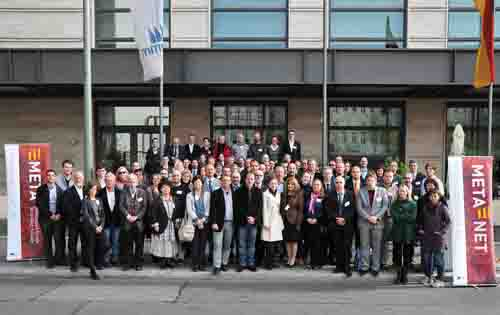
\includegraphics[width=\textwidth]{../_media/meta-net_team.jpg}
   \fbox{Dummy -- we'll include the group photo of our META-NET meeting in Berlin here}
  \caption{Apie šimtą kalbos technologijų ekspertų -- META-NET tinkle dalyvaujančių šalių ir kalbų atstovų -- diskutavo ir apibendrino Baltųjų knygų serijos rezultatus META-NET susitikime Berlyne (2011 m. spalio 21–22 d.) --- \textcolor{grey1}{About 100 language technology experts -- representatives of the countries and languages represented in META-NET -- discussed and finalised the key results and messages of the White Paper Series at a META-NET meeting in Berlin, Germany, on October 21/22, 2011.}}
\end{figure*}

\cleardoublepage

\bsection[META-NET Baltųjų knygų serija -- The META-NET White Paper Series]{META-NET Baltųjų knygų serija --- The META-NET\ \ \ \ \ \ White Paper Series}
\label{whitepaperseries}

\vspace*{-5mm}
\centering
  \setlength{\tabcolsep}{2em}
  \begin{tabularx}{\textwidth}{lllll} \toprule\addlinespace
  %\begin{tabulary}{170mm}{LLL} \toprule
  &Airių & Irish & Gaeilge& \\
  &Anglų & English & English& \\
  &Baskų & Basque & euskara& \\
  &Bulgarų & Bulgarian & български& \\
  &Čekų & Czech & čeština& \\
  &Danų & Danish & dansk& \\
  &Estų & Estonian & eesti& \\
  &Galisų & Galician & galego& \\
  &Graikų & Greek & ελληνικά& \\
  &Islandų & Icelandic & íslenska& \\
  &Ispanų & Spanish & español& \\
  &Italų & Italian & italiano& \\
  &Katalonų & Catalan & català& \\
  &Kroatų & Croatian & hrvatski& \\
  &Latvių & Latvian & latviešu valoda& \\
  &Lenkų & Polish & polski& \\
  &Lietuvių & Lithuanian & lietuvių kalba& \\
  &Maltiečių & Maltese & Malti& \\
  &Norvegų Bokmål & Norwegian Bokmål & bokmål& \\
  &Norvegų Nynorsk & Norwegian Nynorsk & nynorsk& \\
  &Olandų & Dutch & Nederlands& \\
  &Portugalų & Portuguese & português& \\
  &Prancūzų & French & français& \\
  &Rumunų & Romanian & română& \\
  &Serbų & Serbian & српски& \\
  &Slovakų & Slovak & slovenčina& \\
  &Slovėnų & Slovene & slovenščina& \\
  &Suomių & Finnish & suomi& \\
  &Švedų & Swedish & svenska& \\
  &Vengrų & Hungarian & magyar& \\ 
  &Vokiečių & German & Deutsch& \\\addlinespace \bottomrule
\end{tabularx}

\end{document}